\documentclass[spanish,12pt, a4paper,twoside]{paper}

\let\oldsection\section
\def\section{\cleardoublepage\oldsection}

\usepackage{afterpage}

\newcommand\blankpage{%
    \null
    \thispagestyle{empty}%
    \addtocounter{page}{-1}%
    \newpage}

\usepackage{color}
\usepackage{ifthen}
\usepackage{ifpdf}
\usepackage[headings]{fullpage}
\usepackage{listings}
\lstset{language=Java,breaklines=true}
\ifpdf \usepackage[pdftex, pdfpagemode={UseOutlines},bookmarks,colorlinks,linkcolor={blue},plainpages=false,pdfpagelabels,citecolor={red},breaklinks=true]{hyperref}
  \usepackage[pdftex]{graphicx}
  \pdfcompresslevel=9
  \DeclareGraphicsRule{*}{mps}{*}{}
\else
  \usepackage[dvips]{graphicx}
\fi

\newcommand{\entityintro}[3]{%
  \hbox to \hsize{%
    \vbox{%
      \hbox to .2in{}%
    }%
    {\bf  #1}%
    \dotfill\pageref{#2}%
  }
  \makebox[\hsize]{%
    \parbox{.4in}{}%
    \parbox[l]{5in}{%
      \vspace{1mm}%
      #3%
      \vspace{1mm}%
    }%
  }%
}
\newcommand{\refdefined}[1]{
\expandafter\ifx\csname r@#1\endcsname\relax
\relax\else
{$($in \ref{#1}, page \pageref{#1}$)$}\fi}
\date{null}
\title{TweetSCCore Javadoc}
\author{Javier Moreno}
\chardef\textbackslash=`\\


\usepackage[textwidth=15cm, textheight=22.5cm, top=3.5cm, bottom=3.5cm,left= 4cm,right=2cm]{geometry}

\usepackage[spanish, activeacute]{babel}
%\usepackage[applemac]{inputenc} 
\usepackage[utf8]{inputenc}

\usepackage{graphicx}
\usepackage{graphics}
\usepackage{amsmath,amssymb}
\usepackage{float}
\usepackage{changepage}
\usepackage{subcaption}

\usepackage{url}
\usepackage{hyperref} % For hyperlinks in the PDF

\usepackage{algorithm}
\usepackage{multirow}


\begin{document}
%\maketitle
%\thispagestyle{empty}
\begin{titlepage}

\newcommand{\HRule}{\rule{\linewidth}{0.5mm}} % Defines a new command for the horizontal lines, change thickness here

\center % Center everything on the page
 
%	HEADING SECTIONS

\includegraphics[width=2.25cm]{recursos/logoFi.png}
  \hspace{8cm}

\includegraphics[width=2cm]{recursos/logoupm.png}
\\[1cm]

\textsc{\Large Escuela Técnica Superior de Ingenieros Informáticos}\\[0.5cm]
\textsc{\large Universidad Polítecnica de Madrid}
\\[3cm]


%	TITLE SECTION
 \HRule \\[0.4cm]
{ \huge \bfseries TweetSC: Corrector de texto para Twitter}\\[0.4cm] % Title of your document
\HRule \\[2.5cm]

\textsc{\LARGE Trabajo Fin de Máster}\\[0.5cm] 
\textsc{\Large Máster Universitario en Inteligencia Artificial }\\[2.5cm]

 %	AUTHOR SECTION
\begin{flushright}
\large
AUTOR: Javier Moreno Vega\\
TUTOR/ES: Óscar Corcho García y \linebreak
                    Víctor Rodríguez Doncel
\end{flushright}

%\vspace{0.5cm}

%	URL SECTION
{{\url{https://jmorenov.github.io/TweetSC/}}}\\[1cm]

%\vspace{0.5cm}

%	DATE SECTION
{ {\today}}\\[1cm]

\vfill % Fill the rest of the page with whitespace

\end{titlepage}

\afterpage{\blankpage}
\pagenumbering{roman}

%	RESUMEN
\section*{RESUMEN}
Esta memoria explica todo el trabajo desarrollado entrando en detalle en el estado del arte y el  módulo software desarrollado. Primero se realiza una introducción al tema y se exponen los objetivos a realizar. En segundo lugar se presenta el estado del arte sobre el tema de la corrección de textos, específicamente en Twitter y en español. Posteriormente explicamos la solución propuesta con todas sus fases. A continuación se presenta la implementación desarrollada y la documentación del código, además de los recursos utilizados. En siguiente lugar evaluamos los resultados. Y por último se desarrollan las conclusiones y líneas futuras.


%	SUMMARY
\section*{SUMMARY}
This report explains all the work developed by going into detail in the state of the art and the software module developed. First an introduction to the subject is made and the objectives to be made are exposed. Second, the state of the art on the subject of normalization is presented, specifically on Twitter and in Spanish. Later I explain the proposed solution with all its phases. Below is the developed implementation and documentation of the code, in addition to the resources used. Next, we evaluate the results. And finally the conclusions and future lines are developed.


%	ÍNDICE
\tableofcontents % indice de contenidos



%	INDICE DE FIGURAS Y TABLAS
\listoffigures
\listoftables



%	CAPÍTULOS DEL TRABAJO FIN DE MÁSTER
\newpage
\pagenumbering{arabic} 

\section{Introducción}\label{sec:introduccion}
\subsection{Motivación}\label{sec:motivacion}
Los nuevos sistemas de comunicación como la mensajería instantánea, chats, redes sociales han generado un uso diferente de los idiomas en estos ámbitos, llamado lenguaje tipo chat \cite{forsyth:2007}. Una de estas redes sociales y en la que este trabajo va a centrarse es Twitter. En esta red social predomina el Uso de emoticonos, repetición de vocales o eliminación de las mismas, uso abusivo de mayúsculas o asusencia, siglas de expresiones populares; lo que dificulta el análisis de los textos. Las ventajas que ofrece esta red social para investigar sobre ella son la cantidad de datos en tiempo real y su fácil acceso.\\

Uno de los principales problemas a la hora de analizar textos procedentes de las redes sociales son los errores gramaticales que suelen contener, así como la presencia de elementos propios de este tipo de foros que requieren de un procesamiento especial (i.e. hashtags, formas de mencionar a otros usuarios o emoticonos y expresiones habituales en las redes). Además, la limitación en el número de caracteres existente en Twitter la convierte en un caso singular dentro de las redes sociales, ya que los usuarios tienden a adaptar su forma de escribir a dicha limitación, omitiendo palabras y creando abreviaturas que dificultan el uso de herramientas genéricas de procesamiento del lenguaje, especialmente a la hora de realizar tareas como el Análisis de Sentimientos.\\

Los usuarios en Twitter tienden a cometer errores tipográficos, abreviaciones, sustituciones fonéticas y estructuras no gramaticales en los mensajes cortos de texto, causando problemas en las herramientas de análisis. Esto es lo que se consideran palabras mal formadas y la detección de las palabras mal formadas es difícil debido al contexto ruidoso. El objetivo es normalizar estas palabra mal formadas.\\

A parte de un uso puramente de investigación, este tipo de trabajo también es beneficioso para un estudio de marcas o personas y sobre lo que las persones opinan sobre ello en las redes social, ya que sin el proceso de normalización y análisis de sentimientos estaríamos ante millones de datos que costarían mucho trabajo analizar de una forma automática.

\subsection{Objetivos}\label{sec:objetivos}
El objetivo principal de este trabajo es la creación de un corrector que "normalice" tweets en español.\\Para cumplir con este objetivo principal se ha dividido en los siguientes subobjetivos.
\begin{itemize}
\item Acceso a la API de Twitter para obtener tweets.
\item Tokenizar tweets.
\item Detectar entre los tokens las palabras fuera del vocabulario (Out-of-Vocabulary, OOV).
\item Anotar el tipo de palabras OOV.
\item Corregir palabras OOV. 
\end{itemize}
Estos subojetivos se cumplirán con su implementación en un módulo software que además estará disponible en una aplicación web \cite{tweetscweb}.\\

También ejecutaremos este corrector sobre un corpus de tweets disponible en \cite{tweetnorm} y compararemos nuestros resultados con los que se consiguieron en \cite{alegria:2013}.

\subsection{Resumen del documento}\label{sec:resumen}
Esta memoria explica todo el trabajo desarrollado entrando en detalle en el estado del arte y el  módulo software desarrollado. Primero se realiza una introducción al tema y se exponen los objetivos a realizar. En segundo lugar se presenta el estado del arte sobre el tema de la corrección de textos, específicamente en Twitter y en español. Posteriormente explicamos la solución propuesta con todas sus fases. A continuación se presenta la implementación desarrollada y la documentación del código, además de los recursos utilizados. En siguiente lugar evaluamos los resultados. Y por último se desarrollan las conclusiones y líneas futuras.
\section{Estado del arte}\label{sec:estadodelarte}
\subsection{Introducción}\label{sec:introduccion}
En la actualidad, la normalización lingüística de tweets \cite{baldwin:2011} supone un campo de gran interés y en donde la mayoría de trabajos se han realizado sobre textos en inglés y pocos en español. Además no hay ningún trabajo en donde se incluya, dentro de la normalización de tuits, el estudio de los hashtags o etiquetas y los emoticonos, y su contexto. \\
Una introducción al tema de normalización de tuits es el artículo \cite{eisenstein:2013}, donde se revisa el estado del arte en NLP sobre variantes SMS y tweets, y cómo la comunidad científica ha respondido por dos caminos: normalización y adaptación de herramientas.
\subsection{Normalización}\label{sec:normalizacion}
El modelo de canal ruidoso \cite{shannon:1948} ha sido tradicionalmente la primera aproximación a la normalización de textos. Supone que el texto mal formado es T y su forma normalizada es S, por lo que hay que encontrar: arg max $P(S|T)$, calculando arg max $P(T|S) P(S)$, P(S) es el modelo del lenguaje y $P(T|S)$ es el modelo de error. \cite{brillmoore:2000} caracterizan el modelo de error calculando el producto de operaciones de probabilidad en partes de cadenas de caracteres. \cite{toutanovamoore:2002} mejoraron el modelo incorporando información de la pronunciación. \cite{choudhury:2007} modela el proceso de generación de texto a nivel de palabra para mensajes SMS considerando las abreviaturas grafémicas/fonéticas y los errores tipográficos involuntarios como transiciones de estado ocultas del modelo de Markov (HMM) y emisiones, respectivamente. \cite{cookstevenson:2009} expandieron el modelo de error introduciendo inferencias de diferentes procesos de formación erróneos, de acuerdo con la distribución de errores muestreada.\\

Mientras el modelo de canal ruidoso es apropiado para normalización de textos, es difícil aproximar la normalización con exactitud, además estos métodos ignoran el contexto alrededor del OOV, el cual ayuda a resolver ambigüedades. La traducción automática estadística (SMT) se ha propuesto como un medio de normalización de texto sensible al contexto, al tratar el texto mal formado como el idioma de origen, y la forma estándar como el idioma de destino. Por ejemplo \cite{aw:2006}. Normalización de textos como un problema de reconocimiento de voz \cite{kobus:2008}. \cite{beaufort:2002} métodos de estado finitos combinando las ventajas de SMS y el modelo de canal ruidoso. \cite{kaufmannkalita:2010} usan un enfoque de traducción automática con un preprocesador para la normalización sintáctica (en lugar de léxica).\\

El problema de estos trabajos anteriores es que requieren datos de entrenamiento anotados a gran escala, lo que limita su adaptabilidad a nuevos dominios o idiomas, mientras que los trabajos \cite{whitelaw:2009} y \cite{baldwin:2011}, no. Estos trabajos son una buena referencia en el campo de la normalización de tuits en inglés de forma no supervisada. En donde para detectar palabras fuera de diccionario (OOV) utilizan GNU aspell, y los usuarios (@usuario), los hashtags y las URLs son excluidas de la normalización. La normalización tiene relación con los correctores de texto \cite{peterson:1980} pero difiere en que las palabras mal formadas en los mensajes de texto suelen ser intencionadas, para ahorrar caracteres, como identidad social, o debido a la convención en este subgénero de texto. La detección de las palabras mal formadas es difícil debido al contexto ruidoso. El objetivo es normalizar estas palabra mal formadas, además muchas palabras mal formadas son ambiguas y requieren el contexto para poder normalizarlas.

\subsection{Adaptación de herramientas}\label{sec:adaptaciondeherramientas}
En vez de adaptar el texto a herramientas de análisis otro de los caminos a seguir es adaptar las herramientas de análisis al texto. Destacan los trabajos de reconocimiento de voz \cite{gimpel:2011} \cite{owoputi:2013}, reconocimiento de entidades \cite{finin:2010} \cite{ritter:2011} \cite{liu:2011}, análisis gramatical \cite{foster:2011}, modelización de diálogos \cite{ritter:2010} y resumen automático de textos \cite{sharifi:2010}.\\

El reconocimiento de entidades nombradas (NER) es una tarea de extracción de información que busca localizar y clasificar en categorías predefinidas, como personas, organizaciones, lugares, expresiones de tiempo y cantidades, entidades encontradas en un texto. Las soluciones propuestas para NER suelen recaer en tres categorías: Basado en reglas \cite{krupkahausman:1998}, Basada en aprendizaje automático \cite{finkelmanning:2009} \cite{singh:2010} y Métodos híbridos \cite{jansche:2002}. Con la disponibilidad de datos anotados, Enron \cite{minkov:2005} y CoNLL03 \cite{tjong:2003} se han convertidos en los nuevos métodos dominantes. El estudio actual NER se centra principalmente en textos formales, de hecho, el estado del arte actual (CoNLL03) tiene un éxito del 90.8\% en textos formales y 45.8\% en tweets. En el contexto de los textos en Tweets, existe una dificultad en el reconocimiento de entidades nombradas debido a la falta de información y datos de entrenamiento.\\

El trabajo en el contexto de los textos de Twitter se puede dividir en tres categorías: NER en tweets, NER en no tweets y aprendizaje semi-supervisado para NER. El trabajo principal de NER sobre tweets es \cite{finin:2010}, en donde se anotan los tweets y se entrena el modelo con CRF. En cuanto a los trabajos de NER sobre no tweets: \cite{krupkahausman:1998} utilizan reglas manuales para extraer entidades de tipos predefinidos, \cite{zhousu:2002} utilizan HMM (Hidden Markov Model) mientras que \cite{finkel:2005} usa CRF. En la tercera categoría, aprendizaje semi-supervisado para NER, se encuentran los trabajos de \cite{jiangzhai:2007} que utiliza un algoritmo de bootstrapping balanceado, \cite{wu:2009} también utiliza un algoritmo de bootstrapping, \cite{miller:2004} clusters de palabras, \cite{brown:1992} aprende desde texto sin etiquetar y \cite{guo:2009} introduce Latent Semantic Association (LSA) para NER. El trabajo más importante y actual de NER para tweets es \cite{liu:2011} donde replantea el tema de reconocimiento de entidades nombradas en corpus de tuits. Combina un clasificador KNN con CRF (Conditional Random Fields).\\

La desambiguación léxica o etiquetado gramatical (POST) es una parte muy importante y útil en la tarea de normalización de textos ya que nos permite definir el subconjunto de palabras debido a su categoría gramatical que con una probabilidad pueden ser la normalización de un OOV. Además un gran porcentaje de palabras en un texto son palabras que pueden ser asignadas a más de una clase morfológica, a más de un part-of-speech (PoS). Uno de los trabajos más importantes y probado para español es \cite{sanchezforcada:2004}, este trabajo presenta un método de POST de ventana deslizante (SWPoST), asigna el part-of-speech de una palabra basado en la información que dan las palabras en una ventana fija de alrededor. Puede ser implementado como una máquina de estados finitos (Máquina de Mealy).


\subsection{Normalización en espa'nol}\label{sec:normalzacionenespanol}
Una introducción a la normalización de tuits en español es \cite{alegria:2013}\cite{alegria:2015}. Este trabajo propuso en 2013 una tarea o competición en la que los participantes proponían soluciones de normalización de tweets. Los organizadores de la competición ofrecían dos datasets de tweets ya notados uno de desarrollo y otro para test, junto con un tercero que no era público y que era usado para la última evaluación.\\

Las soluciones ofreciddas por los participantes se pueden dividir en dos categorías, los que utilizan generación de candidatos junto un modelo del lenguaje, y los que utilizan transductores o FSTs (Finite State Transducers). El participante que mejor accurancy consiguió, Sistema RAE \cite{porta:2013} con un 0.781, optó por la segunda categoría e implementó un siststem basado en FSTs para la tarea de normalización léxica de mensajes de Twitter en Español. El sistema desarrollado consiste en transductores que se aplican a tokens OOV. Los transductores implementan modelos de variación lingüística que generan conjuntos de candidatos acordes a un léxico. Un modelo estadístico del lenguaje se usa para obtener la secuencia de palabras más probable. El sistema tiene tres componentes principales que se aplican secuencialmente. Un analizador que ejecuta tokenización y análisis léxico sobre palabras en forma estándar y otras expresiones (números, fechas, …). Un componente que genera palabras candidatas para los tokens OOV. Un modelo estadístico del lenguaje para obtener la mejor secuencia de palabras. Y finalmente un truecaser para capitalizar correctamente las palabras asignadas a los tokens OOV. El conjunto de confusión de un token OOV se genera aplicando el algoritmo de camino mínimo a la expresión: $W \circ E \circ L$. Donde W es el automata que representa el token OOV, E es un transductor de editado que genera todas las posibles variaciones de un token, y L es un conjunto de palabras objetivo. Dentro de esta categoría se encuentran los trabajos de la tarea: \cite{ageno:2013} en donde usan una batería de módulos para generar diferentes propuestas de corrección para cada palabra desconocida. La corrección definitiva se elige por votación ponderada según la precisión de cada módulo, \cite{alegria:2013} que además utiliza un modelo para el reconocimiento de voz para la generación de candidatos y \cite{huldenfrancom:2013} presentan dos estrategias basadas en FSTs una con reglas diseñadas manualmente y la otra automática.\\

Entre los participantes que optaron por la primera categoría destaca \cite{ruizcuadros:2013}\cite{vicomtech} que usa reglas de preproceso, un modelo de distancias de edición adecuado al dominio y modelos de lengua para seleccionar candidatos de corrección según el contexto. Su arquitectura está formada por: preproceso basado en expresiones regulares y listas customizadas, generación de candidatos mediante una técnica de mínima de distancia de editado, ranking de candidatos mediante una combinación con pesos de la puntuación del modelo del lenguaje y la distancia de editado y la puntuación del modelo de lenguaje es n-grama utilizando la distancia Levenshtein. El sistema obtuvo resultados superiores a la media en la tarea. Una mejora a este trabajo por los mismos autores es \cite{ruizcuadros:2014} en donde utilizan un sistema basado en reglas para seleccionar los candidatos. Otros trabajos en esta categoría son: \cite{gamallo:2013} que propone un sistema basado en \cite{han:2013}, \cite{saralegi:2013} y \cite{mosqueralopezmoreda:2013} que emplea técnicas de RAH (reconocimiento del habla) mediante la herramienta TENOR \cite{mosquera:2012} junto con un modelo del lenguaje. Otro trabajo basado en la tarea de Tweet-Norm pero que no participó en ella es \cite{ceronguzman:2016}, ellos optaron por normalizar los OOV basándose en similaridad entre grafemas y fonemas; generan el conjunto de confusión (de candidatos) usando grafemas y fonemas, seguido de transductores aplicados mediante reglas para las palabras extranjeras y acentos, la selección de candidatos mediante un modelo del lenguaje con la herramienta Kenlm \cite{heafield:2011}.\\

Fuera de estas dos categorías nos encontramos con los trabajos: \cite{montejo:2013} que utiliza conversiones basadas en reglas hasta una forma final normalizada. Después de recibir una lista con las posibles correcciones el sistema selecciona la más común acorde con una lista de palabras ordenada por frecuencia, \cite{vilares:2013} utilizan una lista de prioridad para los candidatos obtenidos y una tabla de frencuencias de palabrar para puntuarlos, \cite{han:2013} presentan una estrategia basada en búsquedas rápidas mediante una lista de frecuencias aprendida desde un corpus de tweets, \cite{munozgarcia:2013} no generan candidatos simplemente selecciona palabras OOV y las corrigen con un corrector externo y \cite{cotelo:2013} generan candidatos y seleccionan el mejor mediante una función de distancia. Una mejora a este último trabajo por parte de los autores fue \cite{cotelocruz:2015} donde añaden un modulo de puntuación para la selección de candidatos. \\

Otros trabajos sobre normalización en español son \cite{mosquera:2012} en donde se generan candidatos con indexación fonética y se seleccionan el candidato calculando la similaridad léxica junto con un modelo del lenguaje trigrama y \cite{oliva:2011}. Estos trabajos son principalmente sobre mensajes SMS, y no abordan la normalización de tuits en su conjunto. Dentro de la normalización en español existen otras tareas relacionadas como es la tokenización y aquí destaca el trabajo \cite{gomezhidalgo:2013} que estudia la tokenización de textos SMS.

\subsection{Word2Vec}\label{sec:word2vec}
Muchos sistemas y técnicas actuales de NLP tratan las palabras como unidades atómicas, no hay noción de similaridad entre palabras y son representadas como índices en un vocabulario, por ejemplo el modelo N-grama, para tratar de resolver este problema aparecen las representaciones continuas de palabras. Las representaciones continuas de palabras entrenadas sobre corpus sin etiquetas son útiles para muchos trabajos de NLP. Muchos tipos diferentes de modelos han sido propuestos para estimar representaciones continuas de palabras, incluyendo Latent Semantic Analysis (LSA) y Latent Dirichlet Allocation (LDA). En este trabajo se centran en las representaciones distribuidas de palabras aprendidas por redes neuronales, ya que se demostró que su eficacia era considerablemente mejor que LSA para preservar regularidades lineales entre palabras, LDA además es computacionalmente caro en datasets grandes. Además se ha demostrado las redes neuronales basadas en modelos del lenguaje mejoran significativamente los modelos N-grama \cite{bengio:2003} \cite{mikolov:2011} \cite{schwenk:2007}.\\

Los dos modelos de redes neuronales que destacan basados en modelos del lenguaje son: Feedforward Neural Net Language Model (NNLM) \cite{bengio:2003} y Recurrent Neural Net Language Model (RNNLM) que mejora algunas limitaciones de NNLM. El problema de estos modelos es que con grandes cantidades de datos son muy costotos computacionalmente. Para resolver este problema en el trabajo \cite{mikolov:2013} desarrollado por Google se presentaron dos nuevos modelos de arquitecturas para calcular representaciones continuas de vectores de palabras a partir de grandes datasets, además crearon un framework de bibliotecas llamado Word2Vec \cite{google:word2vec}. El principal objetivo de este trabajo es introducir técnicas que puedan ser usadas para aprender vectores de palabras de gran calidad a partir de grandes datasets con millones de palabras y con millones de palabras en el vocabulario. Decidieron explorar modelos más simples que aunque no puedan representar los datos de forma tan precisa como las redes neuronales pero pueden ser entrenados con muchos más datos de forma más eficiente. Estos modelos son: Continuous Baf-of-Words model (CBOW) similar a NNLM, la capa oculta no-lineal se elimina y la capa de proyección es compartida por todas las palabras; y Continuous Skip-gram model similar a CBOW pero en vez de predecir la palabra actual basándose en el contexto intenta maximizar la clasificación de la palabra basándose en otra palabra de la misma frase.\\

La mayoría de las técnicas de representación continua de vectores de palabras representan cada palabra del vocabulario como un vector distinto, sin parámetros compartidos. En particular se ignora la estructura interna de las palabras lo que es una importante limitación en lenguajes ricos morfológicamente. Para intentar resolver este problema en el trabajo \cite{bojanowski:2017}, desarrollado por Facebook \cite{facebook:fasttext} y llamado fastText, se propone un nuevo enfoque basado en el modelo skipgram \cite{mikolov:2013} donde cada palabra se representa como una bolsa de caracteres n-gramas. Una representación de vector está asociada con cada caracter n-grama, las palabras se representan como la suma de estas representaciones. Al usar una representación de vector distinta para cada palabra, el modelo skipgram ignora la estructura interna de las palabras y en este nuevo trabajo se implementa una función de puntuación diferente para tener en cuenta esta información.

\section{Solución propuesta}\label{sec:solucionpropuesta}
La solución propuesta y a la que hemos llamado TweetSC (Tweet Spell Checker) \cite{tweetscweb} se llegó a ella a partir de varios análisis y evaluaciones que se hicieron con diversas bibliotecas y algoritmos, y todos ellos se pueden encontrar en la solución final para su uso.\\

En la primera versión de nuestra solución se construyó un corrector de texto sencillo basándonos en el creado por Peter Norvig \cite{peternorvig}, el cuál utiliza un diccionario para seleccionar las palabras incorrectas y las corrige mediante el teorema de Bayes usando probabilidades. Se usa la fórmula: $argmax_{c\ \in\  candidates}P(c|w)$, que mediante el teorema de Bayes es equivalente a: $argmax_{c\ \in\  candidates}P(c) P(w|c) / P(w)$, y como P(w) es igual para cada candidato c: $argmax_{c\ \in\  candidates}P(c) P(w|c)$. Esta fórmula trata de seleccionar el candidato de probabilidad máxima para cada palabra. Para calcular la probabilidad se usan dos diccionarios, uno de palabras en Español y otro de nombres propios. Se utilizó esta primera versión como punto de partida para ir creando versiones más avanzadas.\\

El resultado final y por tanto nuestra versión definitiva consiste en un proceso iterativo sobre el tweet que se puede dividir en 6 fases: Tokenización, reglas de preproceso, detección de OOVs, generación de candidatos para cada OOV, ranking de candidatos y postproceso.\\

Además para convertir el sistema en uno más dinámico se ha desarrollado una aplicación web con acceso a la API de Twitter para obtener los tweets mediante querys introducidas en un formulario de nuestra aplicación web.

\subsection{Tokenización}\label{sec:tokenizacion}
Cómo realizan los analizadores léxicos en los compiladores, en la primera fase de nuestro proceso se realiza una tokenización del texto o tweet, un tokenizador genera una salida compuesta de tokens o símbolos.\\

Para mejorar la versión inicial se hizo uso de la biblioteca Stanford NLP \cite{stanfordnlp}. Esta biblioteca creada por Stanford NLP Group ofrece tanto etiquetado gramatical (POS Tagging o POST) cómo deteccion de etiquetas (Named Entity Recognition o NER), nosotros la hemos utilizado para esta fase de tokenización. Además de StanfordNLP para la tokenización hemos utilizado Freeling \cite{freeling}, también se ha añadido al sistema el análisis que ofrece freeling.\\

En esta primera fase se recibe como entrada el texto del tweet y genera una lista de tokens que pasaran a la siguiente fase.

\subsection{Reglas de preprocesado}\label{sec:reglasdepreprocesado}
Una vez que hemos obtenido todos los tokens de un tweet se aplican unas reglas de preproceso para normalizar palabras típicas de la red social, pictogramas, fonogramas, onomatopeyas, números, acrónimos, etc. Tras aplicar estas reglas a los tokens que las acepten, se crean OOVs con estos token, se anotan como variaciones y se eliminan de la lista de tokens para las fases siguientes. Los OOV generados se añaden a la lista final de OOV.

\subsection{Detección de OOV}\label{sec:detecciondeoov}
Esta fase tiene como elementos de entrada los tokens restantes de la fase anterior, y se ejecuta token por token el detector de OOV. Para detectarlos se aplican reglas y se van descartando los tokens que son URLs, usuarios de Twitter, hashtag de Twitter y fechas; los elementos restantes se comparan con tres diccionarios utilizados como recursos: diccionario de español, diccionario de inglés y diccionario de entidades.\\

Los token que se detecten dentro del diccionario de español se descartan como OOV, los que se detecten en el diccionario de inglés se anotan como NoEs (No español o ininteligible) y los que se detecten en el diccionario de entidades se anotan como Correct (palabras correspondientes a una entidad o un nuevo préstamo). Para el resto de token que no han sido aceptados en ninguna regla se crea una lista de OOV y son los que pasaran a la siguiente fase pudiendo al final ser anotados como Variation o NoEs.

\subsection{Generación de candidatos OOV}\label{sec:generaciondecandidatosoov}
La generación de candidatos se puede considerar la primera fase de la corrección en sí, ya que sólo se trabaja con OOV a los que se va a buscar una corrección, en ese caso candidatos para ese OOV.
Esta fase tiene como entrada la lista de OOV que no han sido etiquetados en la fase anterior, es decir, los que pueden ser Variation o NoEs. Para cada OOV se generarán una lista de candidatos con diferentes métodos. Los métodos que hemos utilizado con los nombres que hemos definido son: LevenshteinFST, Metaphone, L\_L, FastTest.

\begin{itemize}
	\item \textbf{LevenshteinFST:} Método que utiliza un FST (Finite State Transducers) para generar variaciones en el OOV con un máximo de distancia de editado según la distancia Levenshtein.
	\item \textbf{Metaphone:} Método que utiliza el algoritmo del metáfono en español \cite{mosquera:2011}. Su funcionamiento consiste en generar los fonemas de todos los diccionarios que hemos utilizado para después comparar el fonema del OOV y seleccionar los de mayor similaridad con los fonemas de los diccionarios.
	\item \textbf{L\_L:} Los candidatos generados con este método son las palabras aceptadas por el lenguaje L(\_L)+.
	\item \textbf{FastText:} Este método hace uso de la biblioteca fastText \cite{facebook:fasttext}, a partir de un modelo generado mediante redes neuronales y representando las palabras de forma continua. Los OOV se convierten a vectores de palabras y se comparan con los vectores del modelo generado para obtener los candidatos más parecidos a partir del la similaridad del coseno.	
\end{itemize}

Estos métodos se ejecutan sobre todos los OOV y generan una lista de candidatos que pasarán a la siguiente fase.

\subsection{Ranking de candidatos}\label{sec:rankingdecandidatos}
El ranking de candidatos es la fase que define la corrección de un OOV, o si no tiene corrección (se anota como NoEs). Para generar este ranking hemos utilizado dos marcadores, uno un modelo del lenguaje N-Gram (Modelo del lenguaje \ref{sec:glosariodeterminos}) mediante la biblioteca OpenNLP \cite{opennlp} y el otro la distancia de editado Damerau-Levenshtein.\\

El marcador N-Gram se realiza mediante la comparación de los candidatos de su puntuación en el modelo del lenguaje, es decir, para cada candidato se calcula su puntuación si fuera el elegido. Para el marcador de la distancia Damerau-Levenshtein se calculan la distancia entre el OOV y cada candidato. Finalmente mediante estas dos puntuaciones se calcula se realiza el ranking de candidatos posicionando primero los candidatos con mejor puntuación en el modelo del lenguaje y menor distancia de editado al OOV.\\

Se ha definido además un umbral mínimo para realizar el ranking, los candidatos que no lo cumplan con los marcadores son eliminados. Al finalizar este proceso para cada OOV se selecciona el mejor candidato del ranking, y se anota como Variation, y si no tuviera candidatos, debido al umbral, se anotan como NoEs.

\subsection{Postproceso}\label{sec:postproceso}
Esta última fase consiste en poner mayúsculas en las palabras que fueran necesarias, así como signos de exclamación e interrogación.

\section{Implementación}\label{sec:implementacion}
En esta sección se pretende explicar toda la implementación software que se ha realizado de nuestra solución. Primero se realizará una introducción comentando lenguajes y herramientas utilizadas. Segundo se explicará dónde encontrar y cómo utilizar nuestro software . Posteriormente la documentación generada del código fuente. Y por último se explicará la aplicación web que se ha desarrollado.

\subsection{Introducción}\label{sec:introduccion}
La implementación se ha realizado en tres módulos o componentes, por una parte tenemos la biblioteca con la funcionalidad necesaria para corregir textos de Twitter, acceder a su API y evaluar los resultados sobre un corpus de tweets; después un modulo que implementa aplicación web y por último otro que ofrece funcionalidad para utilizar la biblioteca desde línea de comandos.\\

El lenguaje principal utilizado en todo el proyecto ha sido Java, con la excepción de Python para los script de evaluación y normalización de archivos de datos, y hemos hecho uso de Google Cloud Engine \cite{googlecloudengine} para que la aplicación web esté disponible para cualquier usuario \cite{tweetscweb:spellchecker}.\\

Nuestro sistema software se ha intentado desarrollar de forma que sea un sistema de procesamiento dinámico pudiendo añadir y quitar funcionalidad de manera sencilla, cualquier algoritmo o método implementado funciona a partir de una clase superior para que se puedan añadir nuevos métodos.\\

El módulo principal del sistema es TweetSCCore que implementa la biblioteca para corregir tweets, acceder a la API de Twitter y evaluar resultados mediante el script ofrecido por Tweet-Norm 2013 \cite{alegria:2013}. Los módulos que funcionan a partir de TweetSCCore son: TweetSCExecutable que implementa la funcionalidad necesaria para ejectar nuestro sistema a partir de línea de comandos, y TweetSCWeb donde se implementa la aplicacion web.\\

Se han implementado dos métodos de corrección o normalización de tweets a los que hemos llamado DictionaryMethod, método preliminar que hace uso de diccionarios y la regla de Bayes, y TweetSCMethod que es nuestro método final con las fases que han sido explicadas.

\begin{figure}[h]
El diagrama de clases del sistema completo se muestra a continuación:
 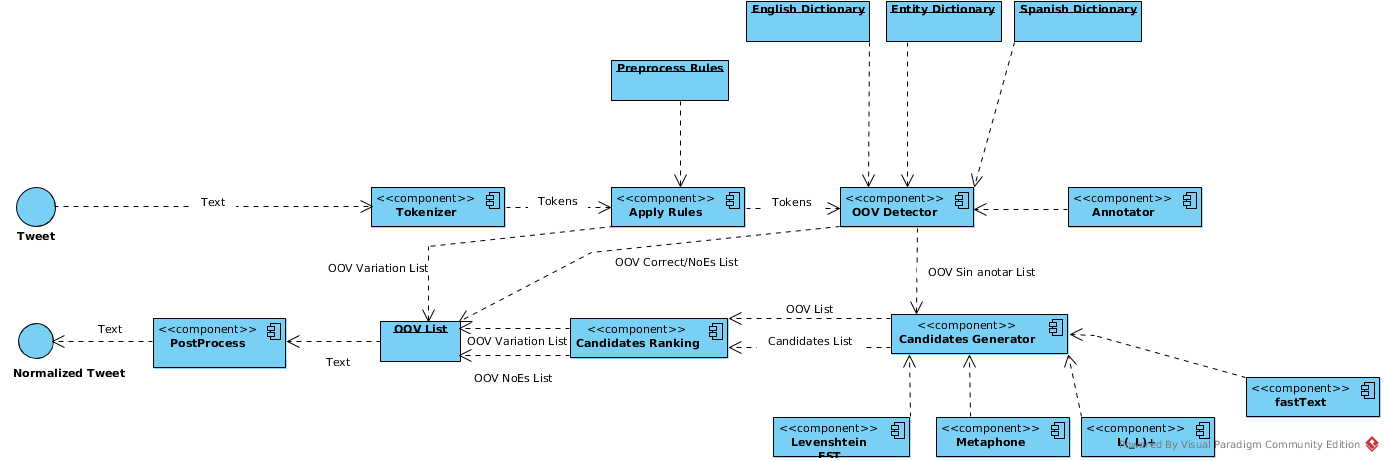
\includegraphics[width=1.2\textwidth]{recursos/DiagramaDelSistema.png}
\caption{Diagrama del sistema}
\label{fig:diagramadelsistema}
\end{figure}

\newpage
\subsection{Cómo usarlo}\label{sec:comousarlo}
Para utilizar nuestro software primero es necesario tener instalado Git y Java 1.8. Después de bajar el código fuente: 
\begin{verbatim}
git clone https://github.com/jmorenov/TweetSC
\end{verbatim}
Posteriormente se compila el código: 
\begin{verbatim}
cd TweetSC/code/
chmod +x build_all.sh
./build_all.sh
\end{verbatim}
Para ejecutarlo desde línea de comandos:
\begin{verbatim}
java -jar tweetscexecutable-all-v0.5.0-alpha.jar -text Texto de prueba
\end{verbatim}
La ejecución de la evaluación sobre el corpus de Tweet-Norm 2013 \cite{alegria:2013}
\begin{verbatim}
java -jar tweetscexecutable-all-v0.5.0-alpha.jar \
    -workingDirectory evaluation \
    -annotatedFile tweet-norm-dev500_annotated.txt \
    -tweetsFile tweet-norm-dev500.txt \
    -resultFile results-test-dev500.txt \
    -method TweetSCMethod
\end{verbatim}
La ejecución de la aplicación web:
\begin{verbatim}
cd tweetscweb
./gradlew run
\end{verbatim}

\subsection{Aplicación web}\label{sec:aplicacionweb}
En esta sección se explicará el funcionamiento de la aplicación web desarrollada y se mostrarán capturas de pantalla de la misma en funcionamiento.\\

La aplicación web se encuentra en nuestro paquete TweetSCWeb y hace uso del framework Spring Boot. Para el backend se utiliza Java y para el frontend Javascript (Jquery). Se ha intentado realizar un diseño sencillo y fluido usando la biblioteca Bootstrap.\\

\begin{figure}[h]
El funcionamiento de la aplicación web es muy sencillo, tiene una sección principal desde la que se accede a las demás secciones mediante una barra de navegación.
\begin{center}
 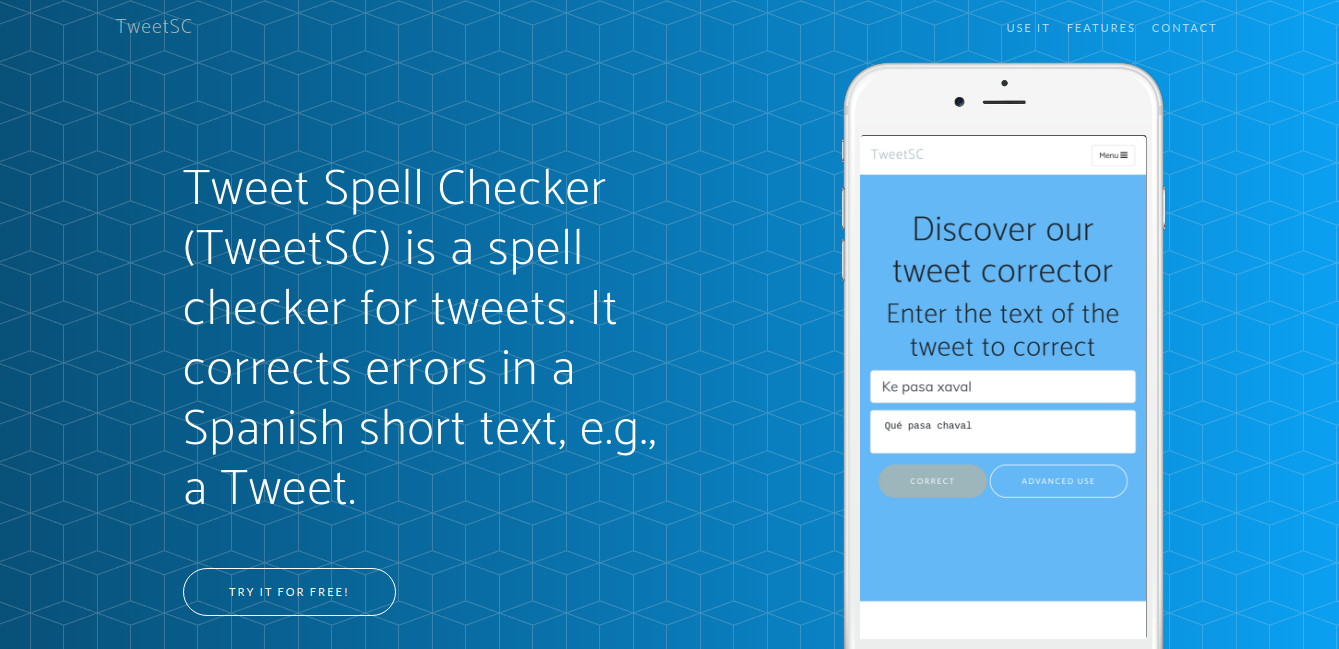
\includegraphics[width=0.9\textwidth]{recursos/WebInicio.png}
\caption{Inicio de la aplicación web}
\label{fig:webinicio}
\end{center}
\end{figure}

\begin{figure}[h]
En la sección siguiente se puede ver un corrector de texto simple.
\begin{center}
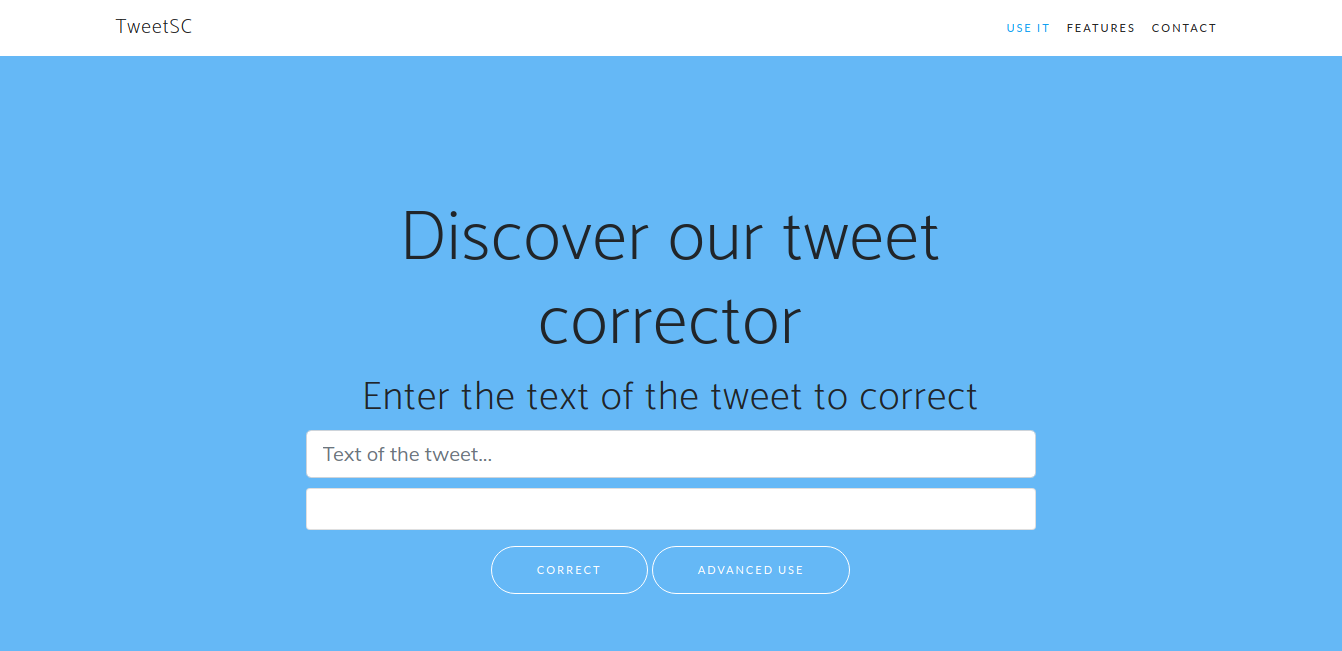
\includegraphics[width=0.9\textwidth]{recursos/WebUseIt.png}
\caption{Sección para utilizar el corrector}
\label{fig:webuseit}
\end{center}
\end{figure}

\begin{figure}[h]
\centering
 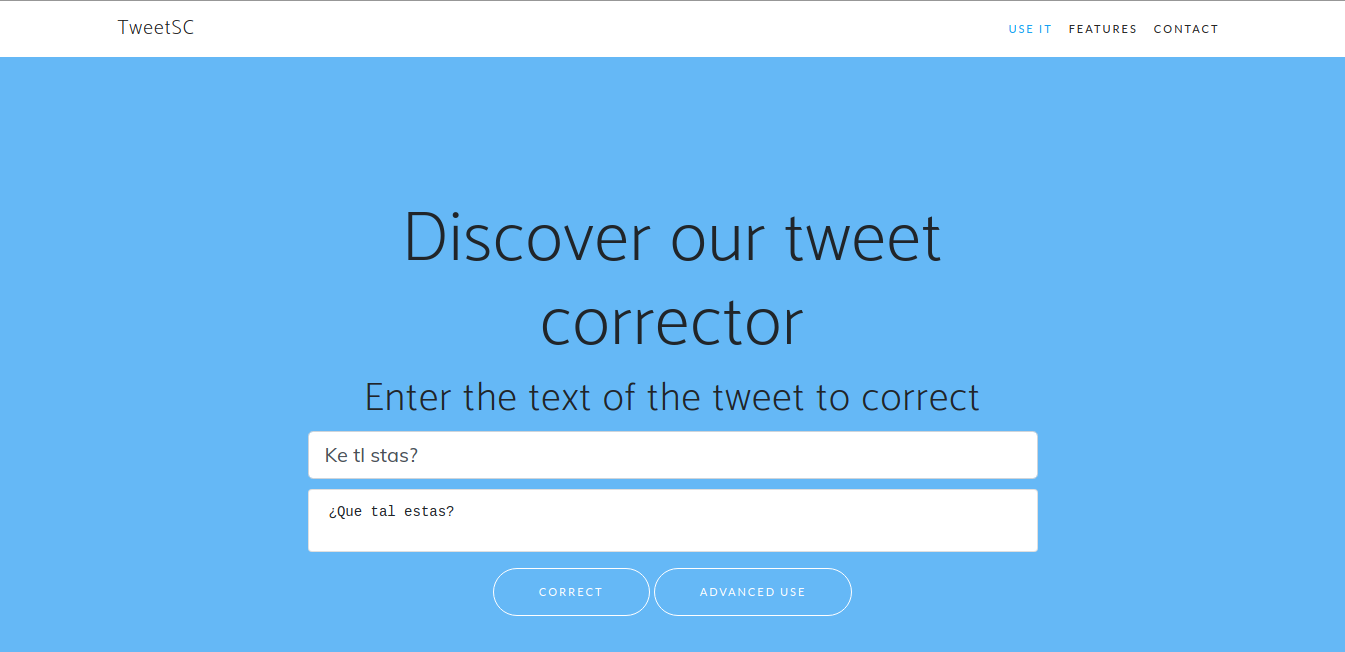
\includegraphics[width=0.9\textwidth]{recursos/WebUseIt_Corrected.png}
\caption{Ejemplo de texto corregido}
\label{fig:webuseitcorrected}
\end{figure}

\begin{figure}[h]
Si accedemos al corrector de uso avanzado podemos buscar tweets mediante texto, usuarios o id del tweet.
\begin{center}
 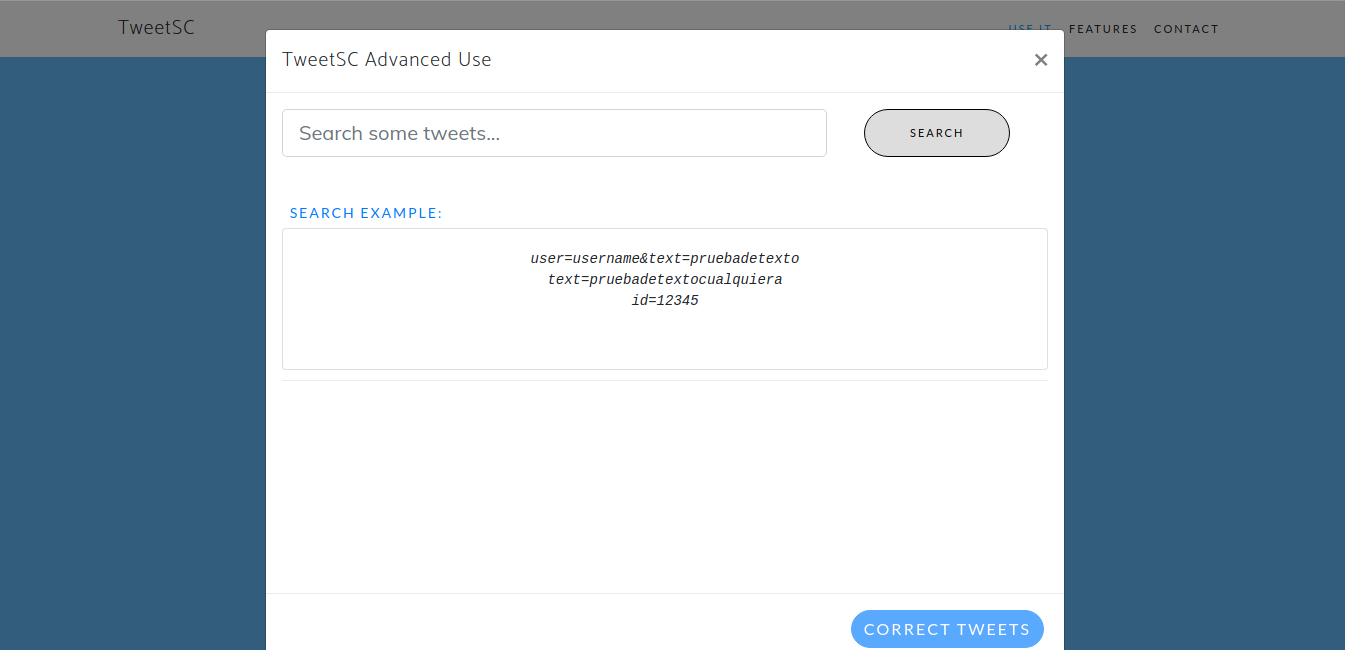
\includegraphics[width=0.9\textwidth]{recursos/WebUseIt_AdvancedUse.png}
\caption{Corrector de tweets uso avanzado}
\label{fig:webuseitadvanceduse}
\end{center}
\end{figure}

\begin{figure}[h]
\centering
 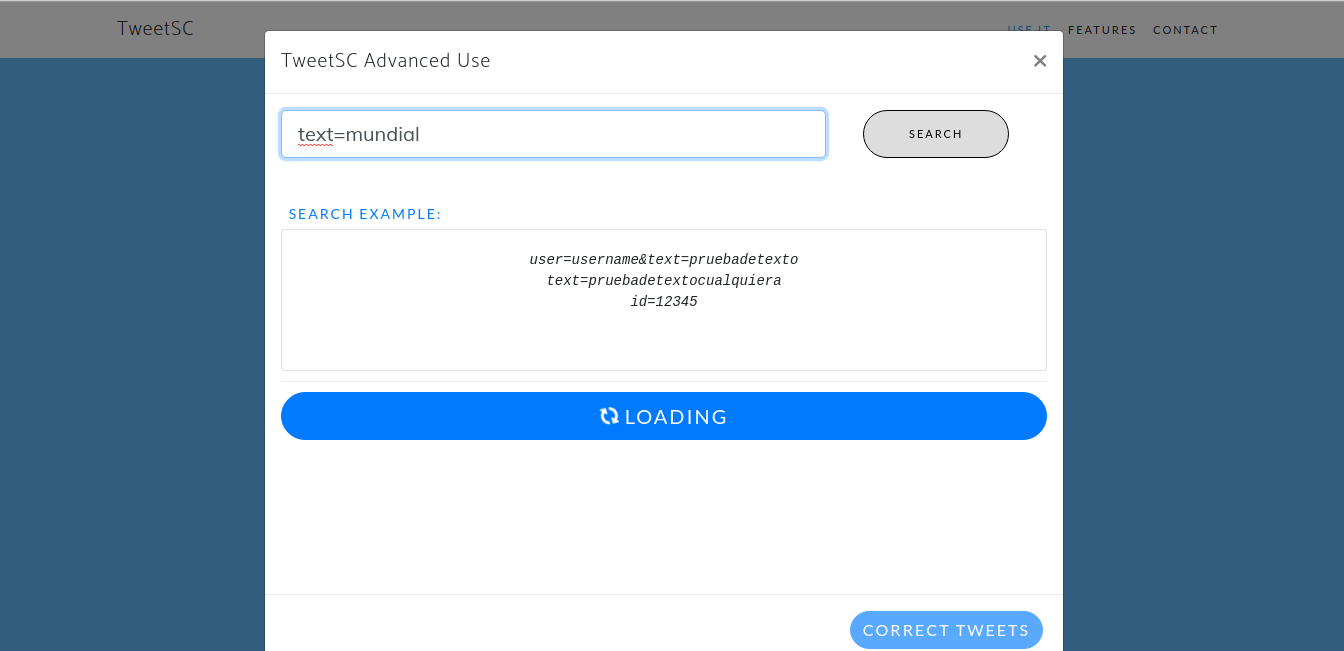
\includegraphics[width=0.9\textwidth]{recursos/WebUseIt_AdvancedUse_Loading.png}
\caption{Ejemplo de búsqueda de tweets}
\label{fig:webuseitadvanceduseloading}
\end{figure}

\begin{figure}[h]
\centering
 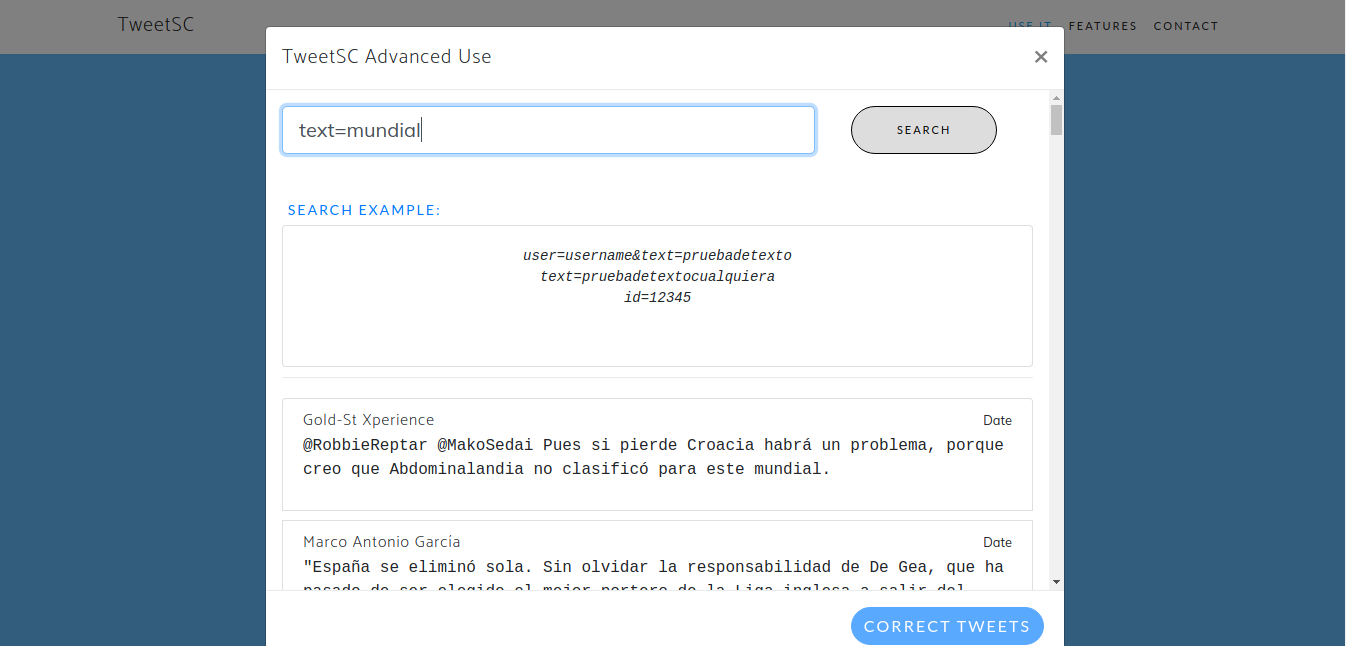
\includegraphics[width=0.9\textwidth]{recursos/WebUseIt_AdvancedUse_SearchResult.png}
\caption{Ejemplo de tweets encontrados}
\label{fig:webuseitadvancedusesearchresult}
\end{figure}

\begin{figure}[h]
Los tweets encontrados se pueden seleccionar para corregirlos.
\begin{center}
 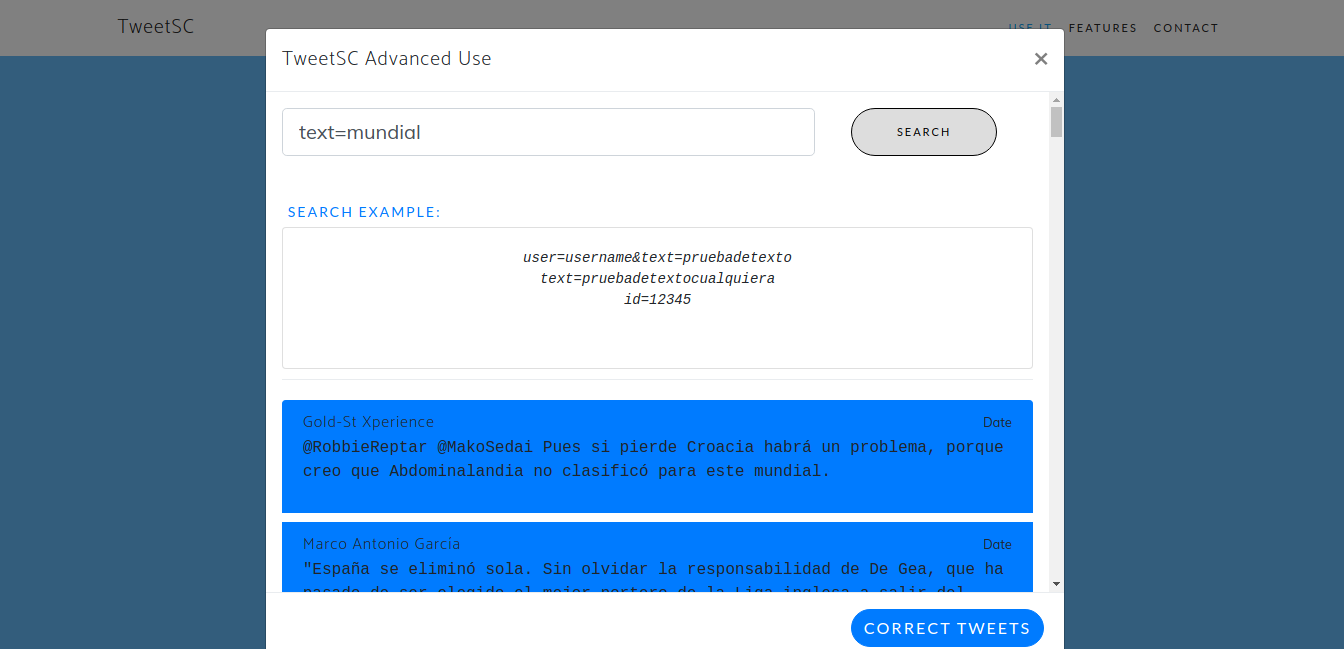
\includegraphics[width=0.9\textwidth]{recursos/WebUseIt_AdvancedUse_TweetsSelected.png}
\caption{Ejemplo de selección de tweets para corregir}
\label{fig:webuseitadvancedusetweetselected}
\end{center}
\end{figure}

\begin{figure}[h]
Cuando los tweets son corregidos se marcan y se muestran ambas versiones, normalizada y la inicial.
\begin{center}
 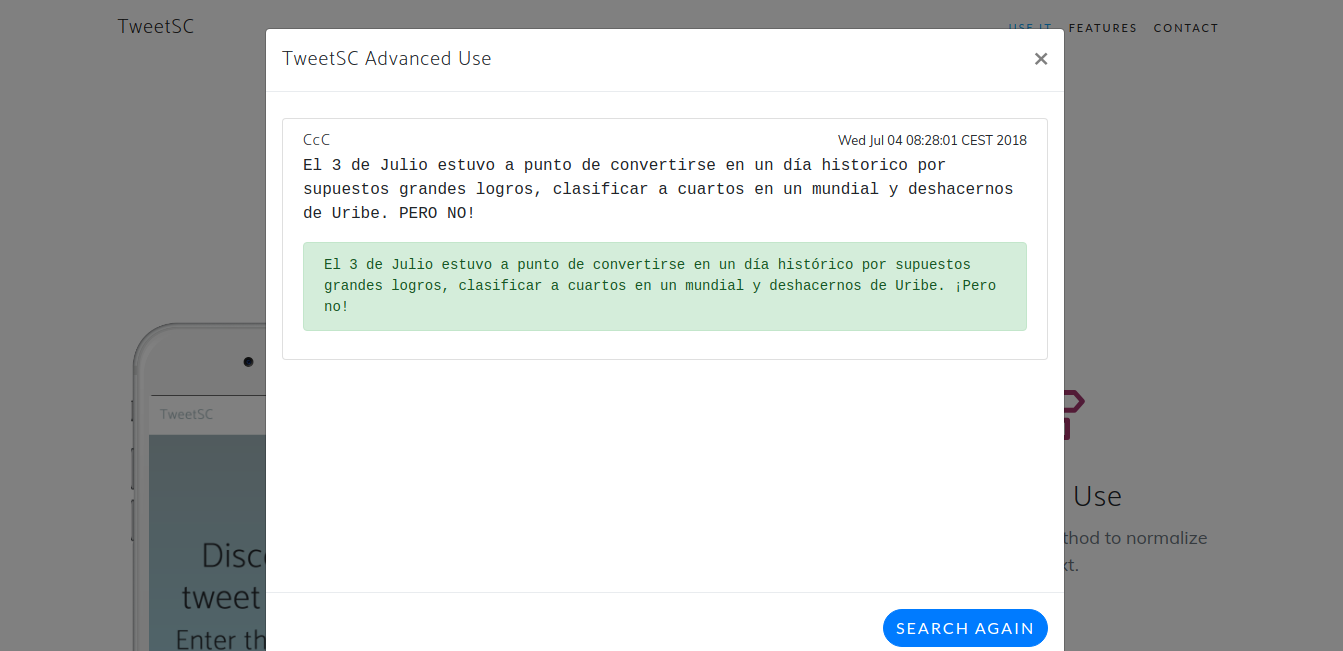
\includegraphics[width=0.9\textwidth]{recursos/WebUseIt_AdvancedUse_TweetCorrected.png}
\caption{Ejemplo de tweets corregidos}
\label{fig:webuseitadvancedusetweetcorrected}
\end{center}
\end{figure}

\begin{figure}[h]
La siguiente sección es la de características del sistema.
\begin{center}
 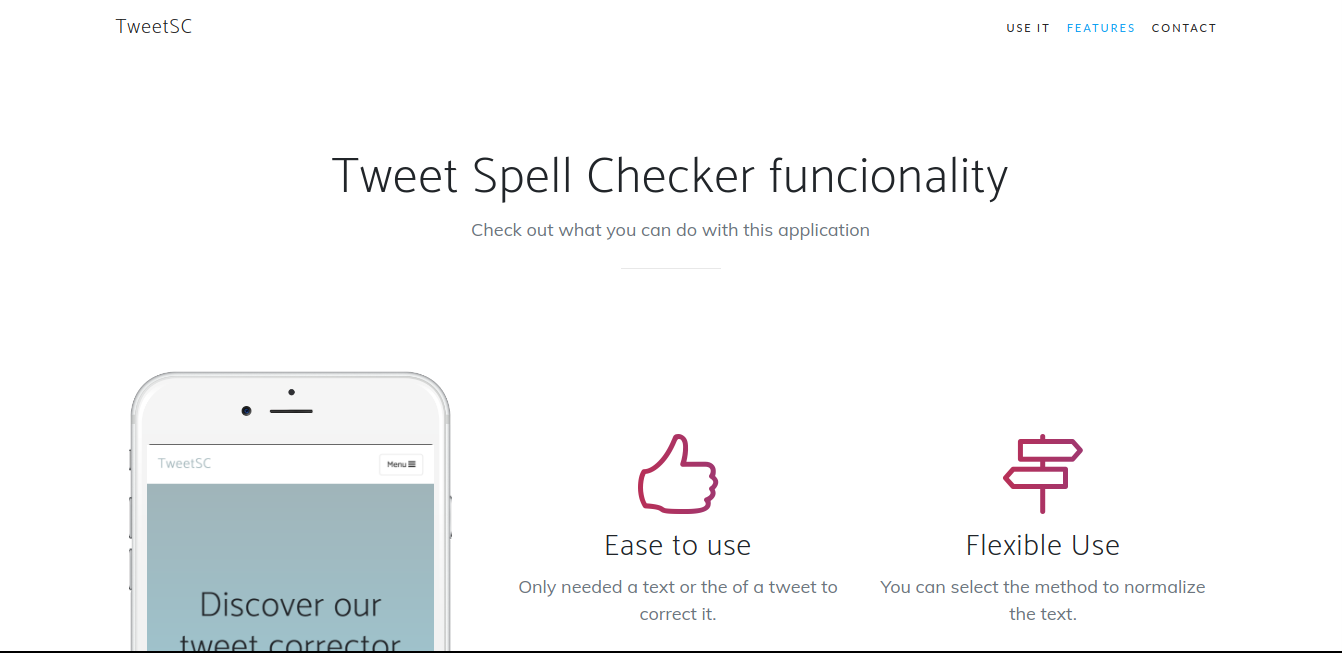
\includegraphics[width=0.9\textwidth]{recursos/WebFeatures1}
\caption{Sección de características de la aplicación web}
\label{fig:webfeatures1}
\end{center}
\end{figure}

\begin{figure}[h]
\centering
 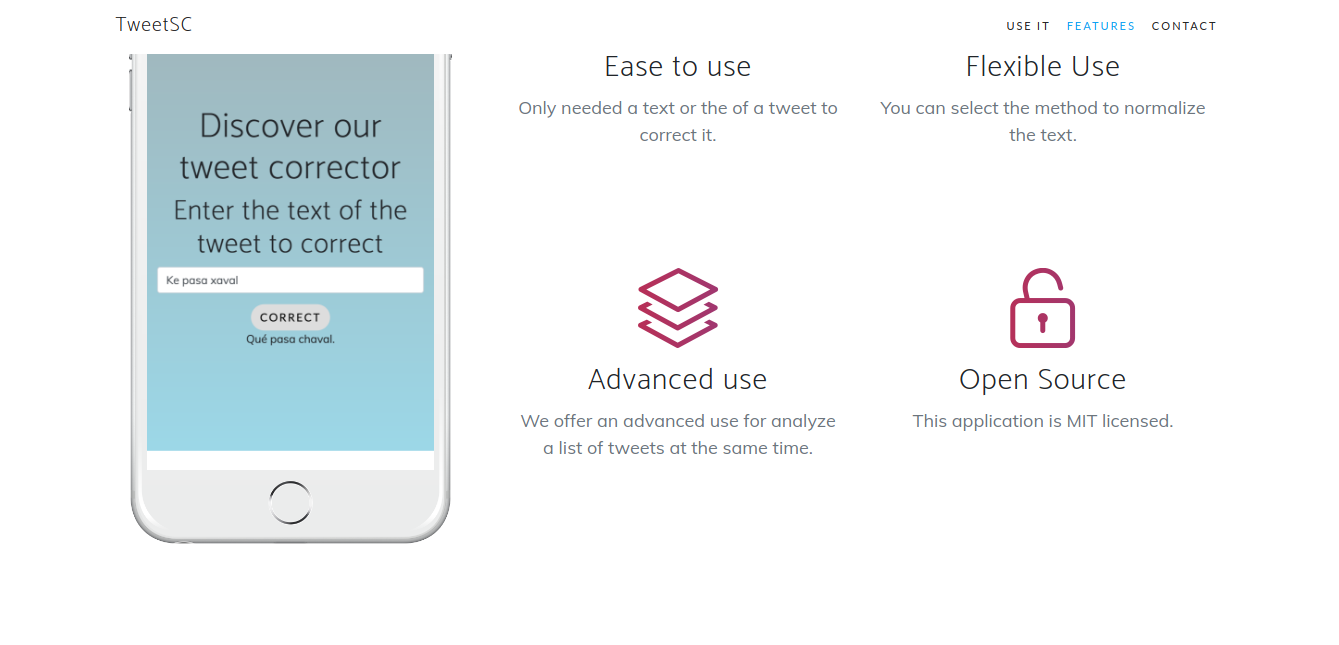
\includegraphics[width=0.9\textwidth]{recursos/WebFeatures2}
\caption{Sección de características de la aplicación web}
\label{fig:webfeatures2}
\end{figure}

\begin{figure}[h]
Además se ha añadido una sección para colaborar mediante GitHub en el desarrollo.
\begin{center}
 
\includegraphics[width=0.9\textwidth]{recursos/WebColaborate}
\caption{Sección de colaboración}
\label{fig:webcolaborate}
\end{center}
\end{figure}

\begin{figure}[h]
Por último la sección de contacto.
\begin{center}
 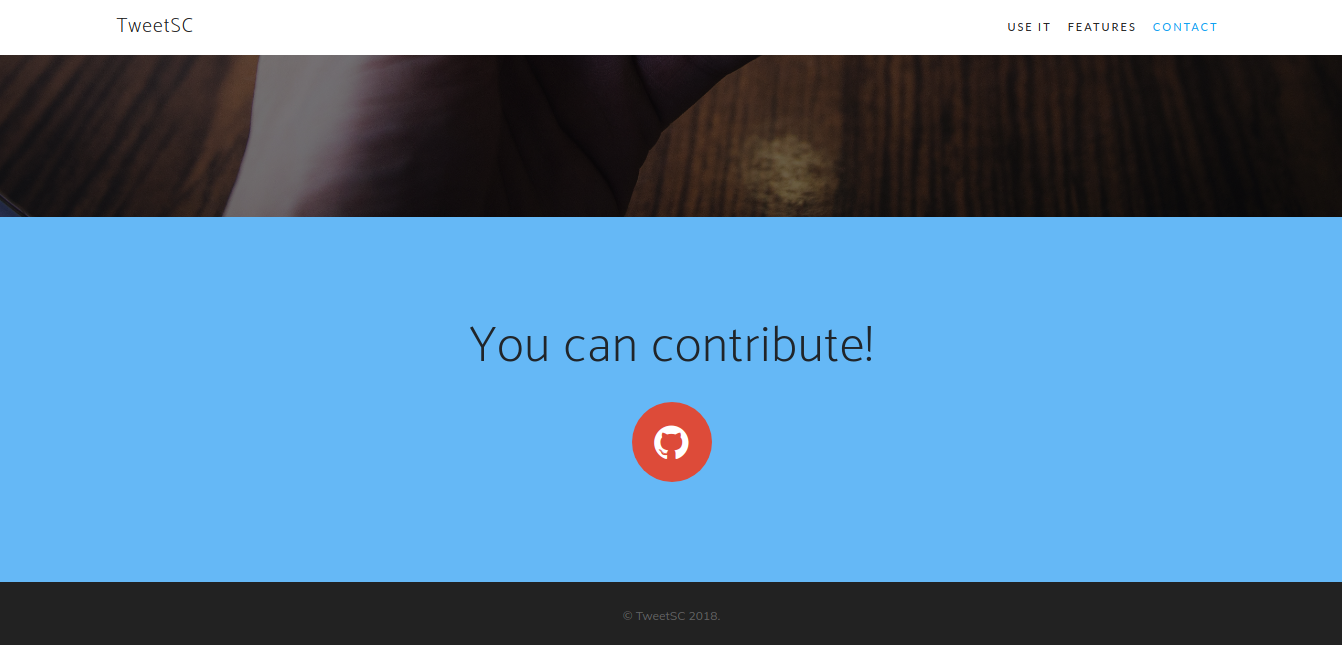
\includegraphics[width=0.9\textwidth]{recursos/WebContact}
\caption{Sección de contacto}
\label{fig:webcontact}
\end{center}
\end{figure}

\section{Recursos utilizados}\label{sec:recursosutilizados}
Los recursos utilizados por nuestro sistema son variados, desde diccionarios hasta bibliotecas para el desarrollo. Empezando desde el paquete TweetSCCore, se ha utilizado la biblioteca StanfordNLP \cite{stanfordnlp} para la tokenización, además está disponible en el paquete la biblioteca Freeling \cite{freeling}. El acceso a la API de Twitter se realiza mediante la bibliteca para Java Twitter4j. La detección de OOV utiliza tres diccionarios, el diccionario de español proporcionado por la herramienta Aspell, el diccionario de entidades JRC y un diccionario de inglés \cite{englishdictionary}. Los métodos de la generación de candidatos utilizan los recursos: Algoritmo del metáfono \cite{mosquera:2011}, fastText \cite{facebook:fasttext} y la biblioteca liblevenshtein \cite{liblevenshtein} para el FST. El ranking de candidatos utiliza la biblioteca \cite{opennlp} para el modelo del lenguaje N-Grama y la distancia Damerau-Levenshtein ofrecida por String.Util de java.\\

Además el corpus de tweets para la evaluación es el que recopiló Tweet-Norm 2013 \cite{alegria:2013} y su script en Python para los resultados.\\

El paquete TweetSCWeb utiliza el framework Spring Boot para la aplicación web junto con el sdk de Google Cloud para ofrecer la aplicación en la nube.

\section{Evaluación}\label{sec:evaluacion}
Esta sección describe la evaluación que se ha hecho de la solución propuesta. Primero se define la metodología utilizada para evaluar la solución, en segundo lugar explicamos el corpus utilizado como datos de entrada, posteriormente el gold standard actual y por último los experimentos que hemos realizada con sus resultados.

\subsection{Metodología}\label{sec:metodologia}
La metodología que hemos seguido ha sido la misma que en la tarea compartida Tweet-Norm 2013 \cite{tweetnorm}. Ellos utilizan como medida de evaluación la corrección de errores, sólo tiene en cuenta si la forma propuesta es correcta en base a los criterios: \textbf{correcta} si la forma original era correcta y no se ha realizado ninguna normalización o si la forma original era incorrecta y el candidato seleccionado es el correcto; \textbf{errónea} en cualquier otro caso. La evaluación final es el número de decisiones realizadas correctamente sobre el total de palabras OOV.

\subsection{Corpus}\label{sec:corpus}
El corpus utilizado es el mismo que en la tarea compartida Tweet-Norm 2013 \cite{tweetnorm}, en donde utilizan dos subconjuntos uno de desarrollo con 500 tweets y otro de evaluación con 600 tweets.

\subsubsection{Gold Standard}\label{sec:goldstandard}
Nuestro gold standard ha sido el sistema propuesto RAE \cite{porta:2013} en Tweet-Norm 2013 \cite{tweetnorm} donde consiguieron un resultado de 0.781 de precisión. Su sistema se basa en trasductores de estados finitos con pesos. 

\subsection{Experimentos}\label{sec:experimentos}
(Experimentos realizados)

\section{Conclusiones}\label{sec:conclusiones}
El proyecto realizado está compuesto de una parte de investigación, cómo se demuestra con el estado del arte y las diferentes soluciones que se han ido realizando hasta llegar a nuestra solución final. Además de la otra parte de desarrollo e implementación de software, ofrenciéndolo para todos en código abierto y en una aplicación web \cite{tweetscweb}.\\

Este desarrollo software se ha dividido en tres componentes o módulos:
\begin{itemize}
	\item TweetSCCore: Núcleo del proyecto con la funcionalidad para corregir textos de Twitter.
	\item TweetSCWeb: Aplicación web para corregir textos.
	\item TweetSCExecutable: Ejecutable java para corregir textos desde línea de comandos.
\end{itemize}
Se puede concluir que nuestro objetivo era construir un corrector de texto para Twitter (\hyperref[sec:objetivos]{sección 1.2}) y se ha conseguido cómo se ha demostrado en las secciones \hyperref[sec:solucionpropuesta]{sección 3} y \hyperref[sec:implementacion]{sección 4}.

\section{Líneas Futuras}\label{sec:lineasfuturas}
Las líneas futuras son muy ámplias ya que estamos en un tema bastante reciente, sobre todo en español cómo se puede ver en el \hyperref[sec:estadodelarte]{sección 2}, y los resultados se pueden mejorar de bastantes formas. Centrándonos en nuestro sistema una mejora futura sería el añadir contexto a los tweets a partir de sus hashtag, usuarios, imágenes o emoticonos; de forma que se pudiera reducir el conjunto de candidatos o añadir nuevos a partir de estos datos. También se podría realizar un análisis de sentimientos sobre el tweet después de normalizar por si se pudiera mejorar la corrección de algún OOV.

\section{TweetSCCore Documentación del código (Java Documentation)}\label{sec:tweetsccorejavadoc}
\subsection*{Class Hierarchy}{
\thispagestyle{empty}
\markboth{Class Hierarchy}{Class Hierarchy}
\addcontentsline{toc}{subsection}{Class Hierarchy}
\subsubsection*{Classes}
{\raggedright
\hspace{0.0cm} $\bullet$ java.lang.Object {\tiny \refdefined{java.lang.Object}} \\
\hspace{1.0cm} $\bullet$ com.jmorenov.tweetsccore.analyzer.AnalysisElement {\tiny \refdefined{com.jmorenov.tweetsccore.analyzer.AnalysisElement}} \\
\hspace{1.0cm} $\bullet$ com.jmorenov.tweetsccore.analyzer.Analyzer {\tiny \refdefined{com.jmorenov.tweetsccore.analyzer.Analyzer}} \\
\hspace{2.0cm} $\bullet$ com.jmorenov.tweetsccore.analyzer.FreelingAnalyzer {\tiny \refdefined{com.jmorenov.tweetsccore.analyzer.FreelingAnalyzer}} \\
\hspace{1.0cm} $\bullet$ com.jmorenov.tweetsccore.candidates.Candidate {\tiny \refdefined{com.jmorenov.tweetsccore.candidates.Candidate}} \\
\hspace{1.0cm} $\bullet$ com.jmorenov.tweetsccore.candidates.CandidatesMethod {\tiny \refdefined{com.jmorenov.tweetsccore.candidates.CandidatesMethod}} \\
\hspace{2.0cm} $\bullet$ com.jmorenov.tweetsccore.candidates.FastTextCandidatesMethod {\tiny \refdefined{com.jmorenov.tweetsccore.candidates.FastTextCandidatesMethod}} \\
\hspace{2.0cm} $\bullet$ com.jmorenov.tweetsccore.candidates.LevenshteinFSTCandidatesMethod {\tiny \refdefined{com.jmorenov.tweetsccore.candidates.LevenshteinFSTCandidatesMethod}} \\
\hspace{2.0cm} $\bullet$ com.jmorenov.tweetsccore.candidates.MetaphoneCandidatesMethod {\tiny \refdefined{com.jmorenov.tweetsccore.candidates.MetaphoneCandidatesMethod}} \\
\hspace{1.0cm} $\bullet$ com.jmorenov.tweetsccore.evaluation.TweetNormEvaluationResult {\tiny \refdefined{com.jmorenov.tweetsccore.evaluation.TweetNormEvaluationResult}} \\
\hspace{1.0cm} $\bullet$ com.jmorenov.tweetsccore.evaluation.TweetNormEvaluator {\tiny \refdefined{com.jmorenov.tweetsccore.evaluation.TweetNormEvaluator}} \\
\hspace{1.0cm} $\bullet$ com.jmorenov.tweetsccore.extra.File {\tiny \refdefined{com.jmorenov.tweetsccore.extra.File}} \\
\hspace{1.0cm} $\bullet$ com.jmorenov.tweetsccore.extra.FreelingInitializator {\tiny \refdefined{com.jmorenov.tweetsccore.extra.FreelingInitializator}} \\
\hspace{1.0cm} $\bullet$ com.jmorenov.tweetsccore.extra.OOV {\tiny \refdefined{com.jmorenov.tweetsccore.extra.OOV}} \\
\hspace{1.0cm} $\bullet$ com.jmorenov.tweetsccore.extra.Parser {\tiny \refdefined{com.jmorenov.tweetsccore.extra.Parser}} \\
\hspace{1.0cm} $\bullet$ com.jmorenov.tweetsccore.method.Method {\tiny \refdefined{com.jmorenov.tweetsccore.method.Method}} \\
\hspace{2.0cm} $\bullet$ com.jmorenov.tweetsccore.method.DictionaryMethod {\tiny \refdefined{com.jmorenov.tweetsccore.method.DictionaryMethod}} \\
\hspace{3.0cm} $\bullet$ com.jmorenov.tweetsccore.method.DictionaryAnalysisMethod {\tiny \refdefined{com.jmorenov.tweetsccore.method.DictionaryAnalysisMethod}} \\
\hspace{1.0cm} $\bullet$ com.jmorenov.tweetsccore.ner.NER {\tiny \refdefined{com.jmorenov.tweetsccore.ner.NER}} \\
\hspace{2.0cm} $\bullet$ com.jmorenov.tweetsccore.ner.StanfordNLPNER {\tiny \refdefined{com.jmorenov.tweetsccore.ner.StanfordNLPNER}} \\
\hspace{1.0cm} $\bullet$ com.jmorenov.tweetsccore.ner.NERELement {\tiny \refdefined{com.jmorenov.tweetsccore.ner.NERELement}} \\
\hspace{1.0cm} $\bullet$ com.jmorenov.tweetsccore.post.FreeLingPOST {\tiny \refdefined{com.jmorenov.tweetsccore.post.FreeLingPOST}} \\
\hspace{1.0cm} $\bullet$ com.jmorenov.tweetsccore.post.OpenNLPPOST {\tiny \refdefined{com.jmorenov.tweetsccore.post.OpenNLPPOST}} \\
\hspace{1.0cm} $\bullet$ com.jmorenov.tweetsccore.post.POST {\tiny \refdefined{com.jmorenov.tweetsccore.post.POST}} \\
\hspace{2.0cm} $\bullet$ com.jmorenov.tweetsccore.post.StanfordNLPPOST {\tiny \refdefined{com.jmorenov.tweetsccore.post.StanfordNLPPOST}} \\
\hspace{1.0cm} $\bullet$ com.jmorenov.tweetsccore.preprocess.ApplyRules {\tiny \refdefined{com.jmorenov.tweetsccore.preprocess.ApplyRules}} \\
\hspace{1.0cm} $\bullet$ com.jmorenov.tweetsccore.preprocess.Rule {\tiny \refdefined{com.jmorenov.tweetsccore.preprocess.Rule}} \\
\hspace{1.0cm} $\bullet$ com.jmorenov.tweetsccore.preprocess.Rules {\tiny \refdefined{com.jmorenov.tweetsccore.preprocess.Rules}} \\
\hspace{1.0cm} $\bullet$ com.jmorenov.tweetsccore.spellchecker.SpellChecker {\tiny \refdefined{com.jmorenov.tweetsccore.spellchecker.SpellChecker}} \\
\hspace{1.0cm} $\bullet$ com.jmorenov.tweetsccore.tokenizer.Tokenizer {\tiny \refdefined{com.jmorenov.tweetsccore.tokenizer.Tokenizer}} \\
\hspace{2.0cm} $\bullet$ com.jmorenov.tweetsccore.tokenizer.FreelingTokenizer {\tiny \refdefined{com.jmorenov.tweetsccore.tokenizer.FreelingTokenizer}} \\
\hspace{2.0cm} $\bullet$ com.jmorenov.tweetsccore.tokenizer.NGramTokenizer {\tiny \refdefined{com.jmorenov.tweetsccore.tokenizer.NGramTokenizer}} \\
\hspace{2.0cm} $\bullet$ com.jmorenov.tweetsccore.tokenizer.OpenNLPTokenizer {\tiny \refdefined{com.jmorenov.tweetsccore.tokenizer.OpenNLPTokenizer}} \\
\hspace{2.0cm} $\bullet$ com.jmorenov.tweetsccore.tokenizer.StanfordNLPTokenizer {\tiny \refdefined{com.jmorenov.tweetsccore.tokenizer.StanfordNLPTokenizer}} \\
\hspace{1.0cm} $\bullet$ com.jmorenov.tweetsccore.twitter.Tweet {\tiny \refdefined{com.jmorenov.tweetsccore.twitter.Tweet}} \\
\hspace{2.0cm} $\bullet$ com.jmorenov.tweetsccore.twitter.TweetCorrected {\tiny \refdefined{com.jmorenov.tweetsccore.twitter.TweetCorrected}} \\
\hspace{1.0cm} $\bullet$ com.jmorenov.tweetsccore.twitter.TwitterConfiguration {\tiny \refdefined{com.jmorenov.tweetsccore.twitter.TwitterConfiguration}} \\
\hspace{1.0cm} $\bullet$ com.jmorenov.tweetsccore.twitter.api.Search {\tiny \refdefined{com.jmorenov.tweetsccore.twitter.api.Search}} \\
\hspace{1.0cm} $\bullet$ java.lang.Enum {\tiny \refdefined{java.lang.Enum}} \\
\hspace{2.0cm} $\bullet$ com.jmorenov.tweetsccore.candidates.CandidatesMethodType {\tiny \refdefined{com.jmorenov.tweetsccore.candidates.CandidatesMethodType}} \\
\hspace{2.0cm} $\bullet$ com.jmorenov.tweetsccore.extra.Annotation {\tiny \refdefined{com.jmorenov.tweetsccore.extra.Annotation}} \\
}
}
\subsection{Package com.jmorenov.tweetsccore.preprocess}{
\label{com.jmorenov.tweetsccore.preprocess}\hypertarget{com.jmorenov.tweetsccore.preprocess}{}
\hskip -.05in
\hbox to \hsize{\textit{ Package Contents\hfil Page}}
\vskip .13in
\hbox{{\bf  Classes}}
\entityintro{ApplyRules}{com.jmorenov.tweetsccore.preprocess.ApplyRules}{ApplyRules class to apply preprocess rules.}
\entityintro{Rule}{com.jmorenov.tweetsccore.preprocess.Rule}{Rule class that define a rule element.}
\entityintro{Rules}{com.jmorenov.tweetsccore.preprocess.Rules}{Rule class that define the Rules element.}
\vskip .1in
\vskip .1in
\subsubsection{\label{com.jmorenov.tweetsccore.preprocess.ApplyRules}Class ApplyRules}{
\hypertarget{com.jmorenov.tweetsccore.preprocess.ApplyRules}{}\vskip .1in 
ApplyRules class to apply preprocess rules.\vskip .1in 
\subsubsection{Declaration}{
\begin{lstlisting}[frame=none]
public class ApplyRules
 extends java.lang.Object\end{lstlisting}
\subsubsection{Constructor summary}{
\begin{verse}
\hyperlink{com.jmorenov.tweetsccore.preprocess.ApplyRules()}{{\bf ApplyRules()}} Constructor of the class.\\
\end{verse}
}
\subsubsection{Method summary}{
\begin{verse}
\hyperlink{com.jmorenov.tweetsccore.preprocess.ApplyRules.apply(java.lang.String)}{{\bf apply(String)}} Method to apply the rules to a text.\\
\end{verse}
}
\subsubsection{Constructors}{
\vskip -2em
\begin{itemize}
\item{ 
\index{ApplyRules()}
\hypertarget{com.jmorenov.tweetsccore.preprocess.ApplyRules()}{{\bf  ApplyRules}\\}
\begin{lstlisting}[frame=none]
public ApplyRules() throws java.io.IOException\end{lstlisting} %end signature
\begin{itemize}
\item{
{\bf  Description}

Constructor of the class.
}
\item{{\bf  Throws}
  \begin{itemize}
   \item{\vskip -.6ex \texttt{java.io.IOException} -- }
  \end{itemize}
}%end item
\end{itemize}
}%end item
\end{itemize}
}
\subsubsection{Methods}{
\vskip -2em
\begin{itemize}
\item{ 
\index{apply(String)}
\hypertarget{com.jmorenov.tweetsccore.preprocess.ApplyRules.apply(java.lang.String)}{{\bf  apply}\\}
\begin{lstlisting}[frame=none]
public java.util.List apply(java.lang.String text)\end{lstlisting} %end signature
\begin{itemize}
\item{
{\bf  Description}

Method to apply the rules to a text.
}
\item{
{\bf  Parameters}
  \begin{itemize}
   \item{
\texttt{text} -- String with the text}
  \end{itemize}
}%end item
\item{{\bf  Returns} -- 
List of OOVs 
}%end item
\end{itemize}
}%end item
\end{itemize}
}
}
\subsubsection{\label{com.jmorenov.tweetsccore.preprocess.Rule}Class Rule}{
\hypertarget{com.jmorenov.tweetsccore.preprocess.Rule}{}\vskip .1in 
Rule class that define a rule element.\vskip .1in 
\subsubsection{Declaration}{
\begin{lstlisting}[frame=none]
public class Rule
 extends java.lang.Object\end{lstlisting}
\subsubsection{Constructor summary}{
\begin{verse}
\hyperlink{com.jmorenov.tweetsccore.preprocess.Rule(java.lang.String, java.lang.String)}{{\bf Rule(String, String)}} Constructor of the class.\\
\end{verse}
}
\subsubsection{Method summary}{
\begin{verse}
\hyperlink{com.jmorenov.tweetsccore.preprocess.Rule.getRegex()}{{\bf getRegex()}} Method to get the regex of the rule.\\
\hyperlink{com.jmorenov.tweetsccore.preprocess.Rule.getResult()}{{\bf getResult()}} Method to get the result of a rule.\\
\end{verse}
}
\subsubsection{Constructors}{
\vskip -2em
\begin{itemize}
\item{ 
\index{Rule(String, String)}
\hypertarget{com.jmorenov.tweetsccore.preprocess.Rule(java.lang.String, java.lang.String)}{{\bf  Rule}\\}
\begin{lstlisting}[frame=none]
public Rule(java.lang.String regex,java.lang.String result)\end{lstlisting} %end signature
\begin{itemize}
\item{
{\bf  Description}

Constructor of the class.
}
\item{
{\bf  Parameters}
  \begin{itemize}
   \item{
\texttt{regex} -- String}
   \item{
\texttt{result} -- String}
  \end{itemize}
}%end item
\end{itemize}
}%end item
\end{itemize}
}
\subsubsection{Methods}{
\vskip -2em
\begin{itemize}
\item{ 
\index{getRegex()}
\hypertarget{com.jmorenov.tweetsccore.preprocess.Rule.getRegex()}{{\bf  getRegex}\\}
\begin{lstlisting}[frame=none]
public java.lang.String getRegex()\end{lstlisting} %end signature
\begin{itemize}
\item{
{\bf  Description}

Method to get the regex of the rule.
}
\item{{\bf  Returns} -- 
String 
}%end item
\end{itemize}
}%end item
\item{ 
\index{getResult()}
\hypertarget{com.jmorenov.tweetsccore.preprocess.Rule.getResult()}{{\bf  getResult}\\}
\begin{lstlisting}[frame=none]
public java.lang.String getResult()\end{lstlisting} %end signature
\begin{itemize}
\item{
{\bf  Description}

Method to get the result of a rule.
}
\item{{\bf  Returns} -- 
String 
}%end item
\end{itemize}
}%end item
\end{itemize}
}
}
\subsubsection{\label{com.jmorenov.tweetsccore.preprocess.Rules}Class Rules}{
\hypertarget{com.jmorenov.tweetsccore.preprocess.Rules}{}\vskip .1in 
Rule class that define the Rules element.\vskip .1in 
\subsubsection{Declaration}{
\begin{lstlisting}[frame=none]
public class Rules
 extends java.lang.Object\end{lstlisting}
\subsubsection{Constructor summary}{
\begin{verse}
\hyperlink{com.jmorenov.tweetsccore.preprocess.Rules(java.lang.String)}{{\bf Rules(String)}} Constructor of the class.\\
\end{verse}
}
\subsubsection{Method summary}{
\begin{verse}
\hyperlink{com.jmorenov.tweetsccore.preprocess.Rules.addRule(com.jmorenov.tweetsccore.preprocess.Rule)}{{\bf addRule(Rule)}} Method to add a new rule.\\
\hyperlink{com.jmorenov.tweetsccore.preprocess.Rules.getRules()}{{\bf getRules()}} Method to get the rules.\\
\end{verse}
}
\subsubsection{Constructors}{
\vskip -2em
\begin{itemize}
\item{ 
\index{Rules(String)}
\hypertarget{com.jmorenov.tweetsccore.preprocess.Rules(java.lang.String)}{{\bf  Rules}\\}
\begin{lstlisting}[frame=none]
public Rules(java.lang.String rulesFilename) throws java.io.IOException\end{lstlisting} %end signature
\begin{itemize}
\item{
{\bf  Description}

Constructor of the class.
}
\item{
{\bf  Parameters}
  \begin{itemize}
   \item{
\texttt{rulesFilename} -- String with the file name of the rules}
  \end{itemize}
}%end item
\item{{\bf  Throws}
  \begin{itemize}
   \item{\vskip -.6ex \texttt{java.io.IOException} -- When the file is not found}
  \end{itemize}
}%end item
\end{itemize}
}%end item
\end{itemize}
}
\subsubsection{Methods}{
\vskip -2em
\begin{itemize}
\item{ 
\index{addRule(Rule)}
\hypertarget{com.jmorenov.tweetsccore.preprocess.Rules.addRule(com.jmorenov.tweetsccore.preprocess.Rule)}{{\bf  addRule}\\}
\begin{lstlisting}[frame=none]
public void addRule(Rule rule)\end{lstlisting} %end signature
\begin{itemize}
\item{
{\bf  Description}

Method to add a new rule.
}
\item{
{\bf  Parameters}
  \begin{itemize}
   \item{
\texttt{rule} -- Rule}
  \end{itemize}
}%end item
\end{itemize}
}%end item
\item{ 
\index{getRules()}
\hypertarget{com.jmorenov.tweetsccore.preprocess.Rules.getRules()}{{\bf  getRules}\\}
\begin{lstlisting}[frame=none]
public java.util.List getRules()\end{lstlisting} %end signature
\begin{itemize}
\item{
{\bf  Description}

Method to get the rules.
}
\item{{\bf  Returns} -- 
List of Rule 
}%end item
\end{itemize}
}%end item
\end{itemize}
}
}
}
\subsection{Package com.jmorenov.tweetsccore.twitter}{
\label{com.jmorenov.tweetsccore.twitter}\hypertarget{com.jmorenov.tweetsccore.twitter}{}
\hskip -.05in
\hbox to \hsize{\textit{ Package Contents\hfil Page}}
\vskip .13in
\hbox{{\bf  Classes}}
\entityintro{Tweet}{com.jmorenov.tweetsccore.twitter.Tweet}{Tweet class with the structure of a tweet.}
\entityintro{TweetCorrected}{com.jmorenov.tweetsccore.twitter.TweetCorrected}{Tweet corrected class with the structure of a corrected tweet.}
\entityintro{TwitterConfiguration}{com.jmorenov.tweetsccore.twitter.TwitterConfiguration}{TwitterConfiguration class with the configuration of the connection with the API of twitter.}
\vskip .1in
\vskip .1in
\subsubsection{\label{com.jmorenov.tweetsccore.twitter.Tweet}Class Tweet}{
\hypertarget{com.jmorenov.tweetsccore.twitter.Tweet}{}\vskip .1in 
Tweet class with the structure of a tweet.\vskip .1in 
\subsubsection{Declaration}{
\begin{lstlisting}[frame=none]
public class Tweet
 extends java.lang.Object\end{lstlisting}
\subsubsection{All known subclasses}{TweetCorrected\small{\refdefined{com.jmorenov.tweetsccore.twitter.TweetCorrected}}}
\subsubsection{Constructor summary}{
\begin{verse}
\hyperlink{com.jmorenov.tweetsccore.twitter.Tweet()}{{\bf Tweet()}} Default constructor of the class.\\
\hyperlink{com.jmorenov.tweetsccore.twitter.Tweet(Status)}{{\bf Tweet(Status)}} Constructor of the class.\\
\hyperlink{com.jmorenov.tweetsccore.twitter.Tweet(java.lang.String, java.lang.String, java.lang.String, java.lang.String)}{{\bf Tweet(String, String, String, String)}} Constructor of the class.\\
\hyperlink{com.jmorenov.tweetsccore.twitter.Tweet(java.lang.String, java.lang.String, java.lang.String, java.lang.String, java.lang.String)}{{\bf Tweet(String, String, String, String, String)}} Constructor of the class.\\
\hyperlink{com.jmorenov.tweetsccore.twitter.Tweet(com.jmorenov.tweetsccore.twitter.Tweet)}{{\bf Tweet(Tweet)}} Copy constructor\\
\end{verse}
}
\subsubsection{Method summary}{
\begin{verse}
\hyperlink{com.jmorenov.tweetsccore.twitter.Tweet.getDate()}{{\bf getDate()}} Method to get the date of the tweet.\\
\hyperlink{com.jmorenov.tweetsccore.twitter.Tweet.getHash()}{{\bf getHash()}} Method to get the hash of the tweet.\\
\hyperlink{com.jmorenov.tweetsccore.twitter.Tweet.getId()}{{\bf getId()}} Method to get the id of the tweet.\\
\hyperlink{com.jmorenov.tweetsccore.twitter.Tweet.getText()}{{\bf getText()}} Method to get the text of the tweet.\\
\hyperlink{com.jmorenov.tweetsccore.twitter.Tweet.getUsername()}{{\bf getUsername()}} Method to get the username of the tweet.\\
\hyperlink{com.jmorenov.tweetsccore.twitter.Tweet.toString()}{{\bf toString()}} Method to get the string of the Tweet.\\
\end{verse}
}
\subsubsection{Constructors}{
\vskip -2em
\begin{itemize}
\item{ 
\index{Tweet()}
\hypertarget{com.jmorenov.tweetsccore.twitter.Tweet()}{{\bf  Tweet}\\}
\begin{lstlisting}[frame=none]
public Tweet()\end{lstlisting} %end signature
\begin{itemize}
\item{
{\bf  Description}

Default constructor of the class.
}
\end{itemize}
}%end item
\item{ 
\index{Tweet(Status)}
\hypertarget{com.jmorenov.tweetsccore.twitter.Tweet(Status)}{{\bf  Tweet}\\}
\begin{lstlisting}[frame=none]
public Tweet(Status tweetStatus)\end{lstlisting} %end signature
\begin{itemize}
\item{
{\bf  Description}

Constructor of the class.
}
\item{
{\bf  Parameters}
  \begin{itemize}
   \item{
\texttt{tweetStatus} -- Status from the object of Twitter4j.}
  \end{itemize}
}%end item
\end{itemize}
}%end item
\item{ 
\index{Tweet(String, String, String, String)}
\hypertarget{com.jmorenov.tweetsccore.twitter.Tweet(java.lang.String, java.lang.String, java.lang.String, java.lang.String)}{{\bf  Tweet}\\}
\begin{lstlisting}[frame=none]
public Tweet(java.lang.String id,java.lang.String username,java.lang.String hash,java.lang.String text)\end{lstlisting} %end signature
\begin{itemize}
\item{
{\bf  Description}

Constructor of the class.
}
\item{
{\bf  Parameters}
  \begin{itemize}
   \item{
\texttt{id} -- String with the id of the tweet.}
   \item{
\texttt{username} -- String with the username of the tweet.}
   \item{
\texttt{hash} -- String with the hash of the tweet.}
   \item{
\texttt{text} -- String with the text of the tweet.}
  \end{itemize}
}%end item
\end{itemize}
}%end item
\item{ 
\index{Tweet(String, String, String, String, String)}
\hypertarget{com.jmorenov.tweetsccore.twitter.Tweet(java.lang.String, java.lang.String, java.lang.String, java.lang.String, java.lang.String)}{{\bf  Tweet}\\}
\begin{lstlisting}[frame=none]
public Tweet(java.lang.String id,java.lang.String username,java.lang.String hash,java.lang.String text,java.lang.String date)\end{lstlisting} %end signature
\begin{itemize}
\item{
{\bf  Description}

Constructor of the class.
}
\item{
{\bf  Parameters}
  \begin{itemize}
   \item{
\texttt{id} -- String with the id of the tweet.}
   \item{
\texttt{username} -- String with the username of the tweet.}
   \item{
\texttt{hash} -- String with the hash of the tweet.}
   \item{
\texttt{text} -- String with the text of the tweet.}
   \item{
\texttt{date} -- String with the date of the tweet.}
  \end{itemize}
}%end item
\end{itemize}
}%end item
\item{ 
\index{Tweet(Tweet)}
\hypertarget{com.jmorenov.tweetsccore.twitter.Tweet(com.jmorenov.tweetsccore.twitter.Tweet)}{{\bf  Tweet}\\}
\begin{lstlisting}[frame=none]
public Tweet(Tweet tweet)\end{lstlisting} %end signature
\begin{itemize}
\item{
{\bf  Description}

Copy constructor
}
\item{
{\bf  Parameters}
  \begin{itemize}
   \item{
\texttt{tweet} -- Tweet to copy from.}
  \end{itemize}
}%end item
\end{itemize}
}%end item
\end{itemize}
}
\subsubsection{Methods}{
\vskip -2em
\begin{itemize}
\item{ 
\index{getDate()}
\hypertarget{com.jmorenov.tweetsccore.twitter.Tweet.getDate()}{{\bf  getDate}\\}
\begin{lstlisting}[frame=none]
public java.lang.String getDate()\end{lstlisting} %end signature
\begin{itemize}
\item{
{\bf  Description}

Method to get the date of the tweet.
}
\item{{\bf  Returns} -- 
String with the date of the tweet. 
}%end item
\end{itemize}
}%end item
\item{ 
\index{getHash()}
\hypertarget{com.jmorenov.tweetsccore.twitter.Tweet.getHash()}{{\bf  getHash}\\}
\begin{lstlisting}[frame=none]
public java.lang.String getHash()\end{lstlisting} %end signature
\begin{itemize}
\item{
{\bf  Description}

Method to get the hash of the tweet.
}
\item{{\bf  Returns} -- 
String with the hash of the tweet. 
}%end item
\end{itemize}
}%end item
\item{ 
\index{getId()}
\hypertarget{com.jmorenov.tweetsccore.twitter.Tweet.getId()}{{\bf  getId}\\}
\begin{lstlisting}[frame=none]
public java.lang.String getId()\end{lstlisting} %end signature
\begin{itemize}
\item{
{\bf  Description}

Method to get the id of the tweet.
}
\item{{\bf  Returns} -- 
String with the id of the tweet. 
}%end item
\end{itemize}
}%end item
\item{ 
\index{getText()}
\hypertarget{com.jmorenov.tweetsccore.twitter.Tweet.getText()}{{\bf  getText}\\}
\begin{lstlisting}[frame=none]
public java.lang.String getText()\end{lstlisting} %end signature
\begin{itemize}
\item{
{\bf  Description}

Method to get the text of the tweet.
}
\item{{\bf  Returns} -- 
String with the text of the tweet. 
}%end item
\end{itemize}
}%end item
\item{ 
\index{getUsername()}
\hypertarget{com.jmorenov.tweetsccore.twitter.Tweet.getUsername()}{{\bf  getUsername}\\}
\begin{lstlisting}[frame=none]
public java.lang.String getUsername()\end{lstlisting} %end signature
\begin{itemize}
\item{
{\bf  Description}

Method to get the username of the tweet.
}
\item{{\bf  Returns} -- 
String with the username of the tweet. 
}%end item
\end{itemize}
}%end item
\item{ 
\index{toString()}
\hypertarget{com.jmorenov.tweetsccore.twitter.Tweet.toString()}{{\bf  toString}\\}
\begin{lstlisting}[frame=none]
public java.lang.String toString()\end{lstlisting} %end signature
\begin{itemize}
\item{
{\bf  Description}

Method to get the string of the Tweet.
}
\item{{\bf  Returns} -- 
String with the String of the Tweet. 
}%end item
\end{itemize}
}%end item
\end{itemize}
}
}
\subsubsection{\label{com.jmorenov.tweetsccore.twitter.TweetCorrected}Class TweetCorrected}{
\hypertarget{com.jmorenov.tweetsccore.twitter.TweetCorrected}{}\vskip .1in 
Tweet corrected class with the structure of a corrected tweet.\vskip .1in 
\subsubsection{Declaration}{
\begin{lstlisting}[frame=none]
public class TweetCorrected
 extends com.jmorenov.tweetsccore.twitter.Tweet\end{lstlisting}
\subsubsection{Constructor summary}{
\begin{verse}
\hyperlink{com.jmorenov.tweetsccore.twitter.TweetCorrected()}{{\bf TweetCorrected()}} Default constuctor of the class.\\
\hyperlink{com.jmorenov.tweetsccore.twitter.TweetCorrected(java.lang.String)}{{\bf TweetCorrected(String)}} Constructor of the class.\\
\hyperlink{com.jmorenov.tweetsccore.twitter.TweetCorrected(java.lang.String, java.lang.String, java.lang.String, java.lang.String, java.lang.String)}{{\bf TweetCorrected(String, String, String, String, String)}} Constructor of the class.\\
\hyperlink{com.jmorenov.tweetsccore.twitter.TweetCorrected(com.jmorenov.tweetsccore.twitter.Tweet)}{{\bf TweetCorrected(Tweet)}} Constructor from tweet.\\
\end{verse}
}
\subsubsection{Method summary}{
\begin{verse}
\hyperlink{com.jmorenov.tweetsccore.twitter.TweetCorrected.computeCorrectedText()}{{\bf computeCorrectedText()}} Method to set the corrected text from the OOV words.\\
\hyperlink{com.jmorenov.tweetsccore.twitter.TweetCorrected.getCorrectedText()}{{\bf getCorrectedText()}} Method to get the corrected tweet.\\
\hyperlink{com.jmorenov.tweetsccore.twitter.TweetCorrected.getOOVWords()}{{\bf getOOVWords()}} Method to get the Out-Of-Vocabulary words of the tweet.\\
\hyperlink{com.jmorenov.tweetsccore.twitter.TweetCorrected.setCorrectedText(java.lang.String)}{{\bf setCorrectedText(String)}} Method to set the corrected tweet.\\
\hyperlink{com.jmorenov.tweetsccore.twitter.TweetCorrected.setOOVWords(java.util.List)}{{\bf setOOVWords(List)}} Method to set the Out-Of-Vocabulary words of the tweet.\\
\hyperlink{com.jmorenov.tweetsccore.twitter.TweetCorrected.toString()}{{\bf toString()}} Method to get the string of the Tweet Corrected.\\
\hyperlink{com.jmorenov.tweetsccore.twitter.TweetCorrected.toTweetNormString()}{{\bf toTweetNormString()}} Method to get the corrected text for Tweet Norm 2013.\\
\end{verse}
}
\subsubsection{Constructors}{
\vskip -2em
\begin{itemize}
\item{ 
\index{TweetCorrected()}
\hypertarget{com.jmorenov.tweetsccore.twitter.TweetCorrected()}{{\bf  TweetCorrected}\\}
\begin{lstlisting}[frame=none]
public TweetCorrected()\end{lstlisting} %end signature
\begin{itemize}
\item{
{\bf  Description}

Default constuctor of the class.
}
\end{itemize}
}%end item
\item{ 
\index{TweetCorrected(String)}
\hypertarget{com.jmorenov.tweetsccore.twitter.TweetCorrected(java.lang.String)}{{\bf  TweetCorrected}\\}
\begin{lstlisting}[frame=none]
public TweetCorrected(java.lang.String text)\end{lstlisting} %end signature
\begin{itemize}
\item{
{\bf  Description}

Constructor of the class.
}
\item{
{\bf  Parameters}
  \begin{itemize}
   \item{
\texttt{text} -- of the tweet}
  \end{itemize}
}%end item
\end{itemize}
}%end item
\item{ 
\index{TweetCorrected(String, String, String, String, String)}
\hypertarget{com.jmorenov.tweetsccore.twitter.TweetCorrected(java.lang.String, java.lang.String, java.lang.String, java.lang.String, java.lang.String)}{{\bf  TweetCorrected}\\}
\begin{lstlisting}[frame=none]
public TweetCorrected(java.lang.String id,java.lang.String username,java.lang.String hash,java.lang.String text,java.lang.String date)\end{lstlisting} %end signature
\begin{itemize}
\item{
{\bf  Description}

Constructor of the class.
}
\item{
{\bf  Parameters}
  \begin{itemize}
   \item{
\texttt{id} -- of the tweet}
   \item{
\texttt{username} -- }
   \item{
\texttt{hash} -- of the tweet}
   \item{
\texttt{text} -- of the tweet}
   \item{
\texttt{date} -- of the tweet}
  \end{itemize}
}%end item
\end{itemize}
}%end item
\item{ 
\index{TweetCorrected(Tweet)}
\hypertarget{com.jmorenov.tweetsccore.twitter.TweetCorrected(com.jmorenov.tweetsccore.twitter.Tweet)}{{\bf  TweetCorrected}\\}
\begin{lstlisting}[frame=none]
public TweetCorrected(Tweet tweet)\end{lstlisting} %end signature
\begin{itemize}
\item{
{\bf  Description}

Constructor from tweet.
}
\item{
{\bf  Parameters}
  \begin{itemize}
   \item{
\texttt{tweet} -- Tweet}
  \end{itemize}
}%end item
\end{itemize}
}%end item
\end{itemize}
}
\subsubsection{Methods}{
\vskip -2em
\begin{itemize}
\item{ 
\index{computeCorrectedText()}
\hypertarget{com.jmorenov.tweetsccore.twitter.TweetCorrected.computeCorrectedText()}{{\bf  computeCorrectedText}\\}
\begin{lstlisting}[frame=none]
public void computeCorrectedText()\end{lstlisting} %end signature
\begin{itemize}
\item{
{\bf  Description}

Method to set the corrected text from the OOV words.
}
\end{itemize}
}%end item
\item{ 
\index{getCorrectedText()}
\hypertarget{com.jmorenov.tweetsccore.twitter.TweetCorrected.getCorrectedText()}{{\bf  getCorrectedText}\\}
\begin{lstlisting}[frame=none]
public java.lang.String getCorrectedText()\end{lstlisting} %end signature
\begin{itemize}
\item{
{\bf  Description}

Method to get the corrected tweet.
}
\item{{\bf  Returns} -- 
String the corrected text 
}%end item
\end{itemize}
}%end item
\item{ 
\index{getOOVWords()}
\hypertarget{com.jmorenov.tweetsccore.twitter.TweetCorrected.getOOVWords()}{{\bf  getOOVWords}\\}
\begin{lstlisting}[frame=none]
public java.util.List getOOVWords()\end{lstlisting} %end signature
\begin{itemize}
\item{
{\bf  Description}

Method to get the Out-Of-Vocabulary words of the tweet.
}
\item{{\bf  Returns} -- 
List of OOV 
}%end item
\end{itemize}
}%end item
\item{ 
\index{setCorrectedText(String)}
\hypertarget{com.jmorenov.tweetsccore.twitter.TweetCorrected.setCorrectedText(java.lang.String)}{{\bf  setCorrectedText}\\}
\begin{lstlisting}[frame=none]
public void setCorrectedText(java.lang.String correctedText)\end{lstlisting} %end signature
\begin{itemize}
\item{
{\bf  Description}

Method to set the corrected tweet.
}
\item{
{\bf  Parameters}
  \begin{itemize}
   \item{
\texttt{correctedText} -- the corrected text}
  \end{itemize}
}%end item
\end{itemize}
}%end item
\item{ 
\index{setOOVWords(List)}
\hypertarget{com.jmorenov.tweetsccore.twitter.TweetCorrected.setOOVWords(java.util.List)}{{\bf  setOOVWords}\\}
\begin{lstlisting}[frame=none]
public void setOOVWords(java.util.List OOVWords)\end{lstlisting} %end signature
\begin{itemize}
\item{
{\bf  Description}

Method to set the Out-Of-Vocabulary words of the tweet.
}
\item{
{\bf  Parameters}
  \begin{itemize}
   \item{
\texttt{OOVWords} -- the list of OOV}
  \end{itemize}
}%end item
\end{itemize}
}%end item
\item{ 
\index{toString()}
\hypertarget{com.jmorenov.tweetsccore.twitter.TweetCorrected.toString()}{{\bf  toString}\\}
\begin{lstlisting}[frame=none]
public java.lang.String toString()\end{lstlisting} %end signature
\begin{itemize}
\item{
{\bf  Description}

Method to get the string of the Tweet Corrected.
}
\item{{\bf  Returns} -- 
String with the String of the class 
}%end item
\end{itemize}
}%end item
\item{ 
\index{toTweetNormString()}
\hypertarget{com.jmorenov.tweetsccore.twitter.TweetCorrected.toTweetNormString()}{{\bf  toTweetNormString}\\}
\begin{lstlisting}[frame=none]
public java.lang.String toTweetNormString()\end{lstlisting} %end signature
\begin{itemize}
\item{
{\bf  Description}

Method to get the corrected text for Tweet Norm 2013.
}
\item{{\bf  Returns} -- 
String with the correctec text. 
}%end item
\end{itemize}
}%end item
\end{itemize}
}
\subsubsection{Members inherited from class Tweet }{
\texttt{com.jmorenov.tweetsccore.twitter.Tweet} {\small 
\refdefined{com.jmorenov.tweetsccore.twitter.Tweet}}
{\small 

\vskip -2em
\begin{itemize}
\item{\vskip -1.5ex 
\texttt{public String {\bf  getDate}()
}%end signature
}%end item
\item{\vskip -1.5ex 
\texttt{public String {\bf  getHash}()
}%end signature
}%end item
\item{\vskip -1.5ex 
\texttt{public String {\bf  getId}()
}%end signature
}%end item
\item{\vskip -1.5ex 
\texttt{public String {\bf  getText}()
}%end signature
}%end item
\item{\vskip -1.5ex 
\texttt{public String {\bf  getUsername}()
}%end signature
}%end item
\item{\vskip -1.5ex 
\texttt{public String {\bf  toString}()
}%end signature
}%end item
\end{itemize}
}
}
\subsubsection{\label{com.jmorenov.tweetsccore.twitter.TwitterConfiguration}Class TwitterConfiguration}{
\hypertarget{com.jmorenov.tweetsccore.twitter.TwitterConfiguration}{}\vskip .1in 
TwitterConfiguration class with the configuration of the connection with the API of twitter.\vskip .1in 
\subsubsection{Declaration}{
\begin{lstlisting}[frame=none]
public class TwitterConfiguration
 extends java.lang.Object\end{lstlisting}
\subsubsection{Method summary}{
\begin{verse}
\hyperlink{com.jmorenov.tweetsccore.twitter.TwitterConfiguration.getInstance()}{{\bf getInstance()}} Method to get the instance of the class.\\
\hyperlink{com.jmorenov.tweetsccore.twitter.TwitterConfiguration.getTwitterAccess()}{{\bf getTwitterAccess()}} Method to get the access to the API.\\
\end{verse}
}
\subsubsection{Methods}{
\vskip -2em
\begin{itemize}
\item{ 
\index{getInstance()}
\hypertarget{com.jmorenov.tweetsccore.twitter.TwitterConfiguration.getInstance()}{{\bf  getInstance}\\}
\begin{lstlisting}[frame=none]
public static TwitterConfiguration getInstance()\end{lstlisting} %end signature
\begin{itemize}
\item{
{\bf  Description}

Method to get the instance of the class.
}
\item{{\bf  Returns} -- 
TwitterConfiguration the instance of the class 
}%end item
\end{itemize}
}%end item
\item{ 
\index{getTwitterAccess()}
\hypertarget{com.jmorenov.tweetsccore.twitter.TwitterConfiguration.getTwitterAccess()}{{\bf  getTwitterAccess}\\}
\begin{lstlisting}[frame=none]
public Twitter getTwitterAccess()\end{lstlisting} %end signature
\begin{itemize}
\item{
{\bf  Description}

Method to get the access to the API.
}
\item{{\bf  Returns} -- 
Twitter 
}%end item
\end{itemize}
}%end item
\end{itemize}
}
}
}
\subsection{Package com.jmorenov.tweetsccore.twitter.api}{
\label{com.jmorenov.tweetsccore.twitter.api}\hypertarget{com.jmorenov.tweetsccore.twitter.api}{}
\hskip -.05in
\hbox to \hsize{\textit{ Package Contents\hfil Page}}
\vskip .13in
\hbox{{\bf  Classes}}
\entityintro{Search}{com.jmorenov.tweetsccore.twitter.api.Search}{Search class to do call on the Twitter API about tweets.}
\vskip .1in
\vskip .1in
\subsubsection{\label{com.jmorenov.tweetsccore.twitter.api.Search}Class Search}{
\hypertarget{com.jmorenov.tweetsccore.twitter.api.Search}{}\vskip .1in 
Search class to do call on the Twitter API about tweets.\vskip .1in 
\subsubsection{Declaration}{
\begin{lstlisting}[frame=none]
public class Search
 extends java.lang.Object\end{lstlisting}
\subsubsection{Constructor summary}{
\begin{verse}
\hyperlink{com.jmorenov.tweetsccore.twitter.api.Search()}{{\bf Search()}} Default constructor of the class.\\
\end{verse}
}
\subsubsection{Method summary}{
\begin{verse}
\hyperlink{com.jmorenov.tweetsccore.twitter.api.Search.getAllTweetsOfUser(java.lang.String)}{{\bf getAllTweetsOfUser(String)}} Method to get all the tweets of an user.\\
\hyperlink{com.jmorenov.tweetsccore.twitter.api.Search.getTweetById(java.lang.String)}{{\bf getTweetById(String)}} Method to search tweets by it id.\\
\hyperlink{com.jmorenov.tweetsccore.twitter.api.Search.getTweetsByText(java.lang.String)}{{\bf getTweetsByText(String)}} Method to search tweets.\\
\hyperlink{com.jmorenov.tweetsccore.twitter.api.Search.getTweetsByTextOfUser(java.lang.String, java.lang.String)}{{\bf getTweetsByTextOfUser(String, String)}} Method to search tweets of an user.\\
\end{verse}
}
\subsubsection{Constructors}{
\vskip -2em
\begin{itemize}
\item{ 
\index{Search()}
\hypertarget{com.jmorenov.tweetsccore.twitter.api.Search()}{{\bf  Search}\\}
\begin{lstlisting}[frame=none]
public Search()\end{lstlisting} %end signature
\begin{itemize}
\item{
{\bf  Description}

Default constructor of the class.
}
\end{itemize}
}%end item
\end{itemize}
}
\subsubsection{Methods}{
\vskip -2em
\begin{itemize}
\item{ 
\index{getAllTweetsOfUser(String)}
\hypertarget{com.jmorenov.tweetsccore.twitter.api.Search.getAllTweetsOfUser(java.lang.String)}{{\bf  getAllTweetsOfUser}\\}
\begin{lstlisting}[frame=none]
public java.util.List getAllTweetsOfUser(java.lang.String username)\end{lstlisting} %end signature
\begin{itemize}
\item{
{\bf  Description}

Method to get all the tweets of an user.
}
\item{
{\bf  Parameters}
  \begin{itemize}
   \item{
\texttt{username} -- the user}
  \end{itemize}
}%end item
\item{{\bf  Returns} -- 
List of Status with the tweets 
}%end item
\end{itemize}
}%end item
\item{ 
\index{getTweetById(String)}
\hypertarget{com.jmorenov.tweetsccore.twitter.api.Search.getTweetById(java.lang.String)}{{\bf  getTweetById}\\}
\begin{lstlisting}[frame=none]
public com.jmorenov.tweetsccore.twitter.Tweet getTweetById(java.lang.String id)\end{lstlisting} %end signature
\begin{itemize}
\item{
{\bf  Description}

Method to search tweets by it id.
}
\item{
{\bf  Parameters}
  \begin{itemize}
   \item{
\texttt{id} -- the id of the tweet}
  \end{itemize}
}%end item
\item{{\bf  Returns} -- 
Status The tweet 
}%end item
\end{itemize}
}%end item
\item{ 
\index{getTweetsByText(String)}
\hypertarget{com.jmorenov.tweetsccore.twitter.api.Search.getTweetsByText(java.lang.String)}{{\bf  getTweetsByText}\\}
\begin{lstlisting}[frame=none]
public java.util.List getTweetsByText(java.lang.String text)\end{lstlisting} %end signature
\begin{itemize}
\item{
{\bf  Description}

Method to search tweets.
}
\item{
{\bf  Parameters}
  \begin{itemize}
   \item{
\texttt{text} -- the text to search}
  \end{itemize}
}%end item
\item{{\bf  Returns} -- 
List of Status with the tweets 
}%end item
\end{itemize}
}%end item
\item{ 
\index{getTweetsByTextOfUser(String, String)}
\hypertarget{com.jmorenov.tweetsccore.twitter.api.Search.getTweetsByTextOfUser(java.lang.String, java.lang.String)}{{\bf  getTweetsByTextOfUser}\\}
\begin{lstlisting}[frame=none]
public java.util.List getTweetsByTextOfUser(java.lang.String username,java.lang.String text)\end{lstlisting} %end signature
\begin{itemize}
\item{
{\bf  Description}

Method to search tweets of an user.
}
\item{
{\bf  Parameters}
  \begin{itemize}
   \item{
\texttt{username} -- the user}
   \item{
\texttt{text} -- the text to search}
  \end{itemize}
}%end item
\item{{\bf  Returns} -- 
List of Status with the tweets 
}%end item
\end{itemize}
}%end item
\end{itemize}
}
}
}
\subsection{Package com.jmorenov.tweetsccore.ner}{
\label{com.jmorenov.tweetsccore.ner}\hypertarget{com.jmorenov.tweetsccore.ner}{}
\hskip -.05in
\hbox to \hsize{\textit{ Package Contents\hfil Page}}
\vskip .13in
\hbox{{\bf  Classes}}
\entityintro{NER}{com.jmorenov.tweetsccore.ner.NER}{POSTagging abstract class.}
\entityintro{NERELement}{com.jmorenov.tweetsccore.ner.NERELement}{NERELement class.}
\entityintro{StanfordNLPNER}{com.jmorenov.tweetsccore.ner.StanfordNLPNER}{StanfordNLP class.}
\vskip .1in
\vskip .1in
\subsubsection{\label{com.jmorenov.tweetsccore.ner.NER}Class NER}{
\hypertarget{com.jmorenov.tweetsccore.ner.NER}{}\vskip .1in 
POSTagging abstract class.\vskip .1in 
\subsubsection{Declaration}{
\begin{lstlisting}[frame=none]
public abstract class NER
 extends java.lang.Object\end{lstlisting}
\subsubsection{All known subclasses}{StanfordNLPNER\small{\refdefined{com.jmorenov.tweetsccore.ner.StanfordNLPNER}}}
\subsubsection{Constructor summary}{
\begin{verse}
\hyperlink{com.jmorenov.tweetsccore.ner.NER()}{{\bf NER()}} \\
\end{verse}
}
\subsubsection{Method summary}{
\begin{verse}
\hyperlink{com.jmorenov.tweetsccore.ner.NER.getNERElements(java.lang.String)}{{\bf getNERElements(String)}} Method to get a list with the NER Elements detected.\\
\end{verse}
}
\subsubsection{Constructors}{
\vskip -2em
\begin{itemize}
\item{ 
\index{NER()}
\hypertarget{com.jmorenov.tweetsccore.ner.NER()}{{\bf  NER}\\}
\begin{lstlisting}[frame=none]
public NER()\end{lstlisting} %end signature
}%end item
\end{itemize}
}
\subsubsection{Methods}{
\vskip -2em
\begin{itemize}
\item{ 
\index{getNERElements(String)}
\hypertarget{com.jmorenov.tweetsccore.ner.NER.getNERElements(java.lang.String)}{{\bf  getNERElements}\\}
\begin{lstlisting}[frame=none]
public abstract java.util.List getNERElements(java.lang.String text)\end{lstlisting} %end signature
\begin{itemize}
\item{
{\bf  Description}

Method to get a list with the NER Elements detected.
}
\item{{\bf  Returns} -- 
List with the NER Elements. 
}%end item
\end{itemize}
}%end item
\end{itemize}
}
}
\subsubsection{\label{com.jmorenov.tweetsccore.ner.NERELement}Class NERELement}{
\hypertarget{com.jmorenov.tweetsccore.ner.NERELement}{}\vskip .1in 
NERELement class.\vskip .1in 
\subsubsection{Declaration}{
\begin{lstlisting}[frame=none]
public class NERELement
 extends java.lang.Object\end{lstlisting}
\subsubsection{Constructor summary}{
\begin{verse}
\hyperlink{com.jmorenov.tweetsccore.ner.NERELement(java.lang.String, java.lang.String)}{{\bf NERELement(String, String)}} Constructor of the class\\
\end{verse}
}
\subsubsection{Method summary}{
\begin{verse}
\hyperlink{com.jmorenov.tweetsccore.ner.NERELement.getNerDetected()}{{\bf getNerDetected()}} Method to get the ner detected.\\
\hyperlink{com.jmorenov.tweetsccore.ner.NERELement.getOriginalElement()}{{\bf getOriginalElement()}} Method to get the original element.\\
\end{verse}
}
\subsubsection{Constructors}{
\vskip -2em
\begin{itemize}
\item{ 
\index{NERELement(String, String)}
\hypertarget{com.jmorenov.tweetsccore.ner.NERELement(java.lang.String, java.lang.String)}{{\bf  NERELement}\\}
\begin{lstlisting}[frame=none]
public NERELement(java.lang.String originalElement,java.lang.String nerDetected)\end{lstlisting} %end signature
\begin{itemize}
\item{
{\bf  Description}

Constructor of the class
}
\item{
{\bf  Parameters}
  \begin{itemize}
   \item{
\texttt{originalElement} -- }
   \item{
\texttt{nerDetected} -- }
  \end{itemize}
}%end item
\end{itemize}
}%end item
\end{itemize}
}
\subsubsection{Methods}{
\vskip -2em
\begin{itemize}
\item{ 
\index{getNerDetected()}
\hypertarget{com.jmorenov.tweetsccore.ner.NERELement.getNerDetected()}{{\bf  getNerDetected}\\}
\begin{lstlisting}[frame=none]
public java.lang.String getNerDetected()\end{lstlisting} %end signature
\begin{itemize}
\item{
{\bf  Description}

Method to get the ner detected.
}
\item{{\bf  Returns} -- 
String with the ner detected 
}%end item
\end{itemize}
}%end item
\item{ 
\index{getOriginalElement()}
\hypertarget{com.jmorenov.tweetsccore.ner.NERELement.getOriginalElement()}{{\bf  getOriginalElement}\\}
\begin{lstlisting}[frame=none]
public java.lang.String getOriginalElement()\end{lstlisting} %end signature
\begin{itemize}
\item{
{\bf  Description}

Method to get the original element.
}
\item{{\bf  Returns} -- 
String with the original element 
}%end item
\end{itemize}
}%end item
\end{itemize}
}
}
\subsubsection{\label{com.jmorenov.tweetsccore.ner.StanfordNLPNER}Class StanfordNLPNER}{
\hypertarget{com.jmorenov.tweetsccore.ner.StanfordNLPNER}{}\vskip .1in 
StanfordNLP class.\vskip .1in 
\subsubsection{Declaration}{
\begin{lstlisting}[frame=none]
public class StanfordNLPNER
 extends com.jmorenov.tweetsccore.ner.NER\end{lstlisting}
\subsubsection{Constructor summary}{
\begin{verse}
\hyperlink{com.jmorenov.tweetsccore.ner.StanfordNLPNER(java.lang.String)}{{\bf StanfordNLPNER(String)}} \\
\end{verse}
}
\subsubsection{Method summary}{
\begin{verse}
\hyperlink{com.jmorenov.tweetsccore.ner.StanfordNLPNER.getNERElements(java.lang.String)}{{\bf getNERElements(String)}} Method to get a list with the NER Elements detected.\\
\end{verse}
}
\subsubsection{Constructors}{
\vskip -2em
\begin{itemize}
\item{ 
\index{StanfordNLPNER(String)}
\hypertarget{com.jmorenov.tweetsccore.ner.StanfordNLPNER(java.lang.String)}{{\bf  StanfordNLPNER}\\}
\begin{lstlisting}[frame=none]
public StanfordNLPNER(java.lang.String text)\end{lstlisting} %end signature
}%end item
\end{itemize}
}
\subsubsection{Methods}{
\vskip -2em
\begin{itemize}
\item{ 
\index{getNERElements(String)}
\hypertarget{com.jmorenov.tweetsccore.ner.StanfordNLPNER.getNERElements(java.lang.String)}{{\bf  getNERElements}\\}
\begin{lstlisting}[frame=none]
public java.util.List getNERElements(java.lang.String text)\end{lstlisting} %end signature
\begin{itemize}
\item{
{\bf  Description}

Method to get a list with the NER Elements detected.
}
\item{{\bf  Returns} -- 
List with the NER Elements. 
}%end item
\end{itemize}
}%end item
\end{itemize}
}
\subsubsection{Members inherited from class NER }{
\texttt{com.jmorenov.tweetsccore.ner.NER} {\small 
\refdefined{com.jmorenov.tweetsccore.ner.NER}}
{\small 

\vskip -2em
\begin{itemize}
\item{\vskip -1.5ex 
\texttt{public abstract List {\bf  getNERElements}(\texttt{java.lang.String} {\bf  text})
}%end signature
}%end item
\end{itemize}
}
}
}
\subsection{Package com.jmorenov.tweetsccore.analyzer}{
\label{com.jmorenov.tweetsccore.analyzer}\hypertarget{com.jmorenov.tweetsccore.analyzer}{}
\hskip -.05in
\hbox to \hsize{\textit{ Package Contents\hfil Page}}
\vskip .13in
\hbox{{\bf  Classes}}
\entityintro{AnalysisElement}{com.jmorenov.tweetsccore.analyzer.AnalysisElement}{AnalysisElement class.}
\entityintro{Analyzer}{com.jmorenov.tweetsccore.analyzer.Analyzer}{Analyzer abstract class.}
\entityintro{FreelingAnalyzer}{com.jmorenov.tweetsccore.analyzer.FreelingAnalyzer}{FreelingTokenizer class to tokenize a text.}
\vskip .1in
\vskip .1in
\subsubsection{\label{com.jmorenov.tweetsccore.analyzer.AnalysisElement}Class AnalysisElement}{
\hypertarget{com.jmorenov.tweetsccore.analyzer.AnalysisElement}{}\vskip .1in 
AnalysisElement class.\vskip .1in 
\subsubsection{Declaration}{
\begin{lstlisting}[frame=none]
public class AnalysisElement
 extends java.lang.Object\end{lstlisting}
\subsubsection{Constructor summary}{
\begin{verse}
\hyperlink{com.jmorenov.tweetsccore.analyzer.AnalysisElement(java.lang.String, java.lang.String, java.lang.String, java.lang.String, boolean)}{{\bf AnalysisElement(String, String, String, String, boolean)}} Constructor of the class.\\
\end{verse}
}
\subsubsection{Method summary}{
\begin{verse}
\hyperlink{com.jmorenov.tweetsccore.analyzer.AnalysisElement.getForm()}{{\bf getForm()}} Method to get the form.\\
\hyperlink{com.jmorenov.tweetsccore.analyzer.AnalysisElement.getLemma()}{{\bf getLemma()}} Method to get the lemma.\\
\hyperlink{com.jmorenov.tweetsccore.analyzer.AnalysisElement.getSenses()}{{\bf getSenses()}} Method to get the senses.\\
\hyperlink{com.jmorenov.tweetsccore.analyzer.AnalysisElement.getTag()}{{\bf getTag()}} Method to get the tag.\\
\hyperlink{com.jmorenov.tweetsccore.analyzer.AnalysisElement.isMultiWord()}{{\bf isMultiWord()}} Method to get if the element is multi word.\\
\hyperlink{com.jmorenov.tweetsccore.analyzer.AnalysisElement.toString()}{{\bf toString()}} Method to get the class as String.\\
\end{verse}
}
\subsubsection{Constructors}{
\vskip -2em
\begin{itemize}
\item{ 
\index{AnalysisElement(String, String, String, String, boolean)}
\hypertarget{com.jmorenov.tweetsccore.analyzer.AnalysisElement(java.lang.String, java.lang.String, java.lang.String, java.lang.String, boolean)}{{\bf  AnalysisElement}\\}
\begin{lstlisting}[frame=none]
public AnalysisElement(java.lang.String form,java.lang.String lemma,java.lang.String tag,java.lang.String senses,boolean isMultiWord)\end{lstlisting} %end signature
\begin{itemize}
\item{
{\bf  Description}

Constructor of the class.
}
\item{
{\bf  Parameters}
  \begin{itemize}
   \item{
\texttt{form} -- }
   \item{
\texttt{lemma} -- }
   \item{
\texttt{tag} -- }
   \item{
\texttt{isMultiWord} -- }
  \end{itemize}
}%end item
\end{itemize}
}%end item
\end{itemize}
}
\subsubsection{Methods}{
\vskip -2em
\begin{itemize}
\item{ 
\index{getForm()}
\hypertarget{com.jmorenov.tweetsccore.analyzer.AnalysisElement.getForm()}{{\bf  getForm}\\}
\begin{lstlisting}[frame=none]
public java.lang.String getForm()\end{lstlisting} %end signature
\begin{itemize}
\item{
{\bf  Description}

Method to get the form.
}
\item{{\bf  Returns} -- 
String with the form 
}%end item
\end{itemize}
}%end item
\item{ 
\index{getLemma()}
\hypertarget{com.jmorenov.tweetsccore.analyzer.AnalysisElement.getLemma()}{{\bf  getLemma}\\}
\begin{lstlisting}[frame=none]
public java.lang.String getLemma()\end{lstlisting} %end signature
\begin{itemize}
\item{
{\bf  Description}

Method to get the lemma.
}
\item{{\bf  Returns} -- 
String with the lemma 
}%end item
\end{itemize}
}%end item
\item{ 
\index{getSenses()}
\hypertarget{com.jmorenov.tweetsccore.analyzer.AnalysisElement.getSenses()}{{\bf  getSenses}\\}
\begin{lstlisting}[frame=none]
public java.lang.String getSenses()\end{lstlisting} %end signature
\begin{itemize}
\item{
{\bf  Description}

Method to get the senses.
}
\item{{\bf  Returns} -- 
String with the senses 
}%end item
\end{itemize}
}%end item
\item{ 
\index{getTag()}
\hypertarget{com.jmorenov.tweetsccore.analyzer.AnalysisElement.getTag()}{{\bf  getTag}\\}
\begin{lstlisting}[frame=none]
public java.lang.String getTag()\end{lstlisting} %end signature
\begin{itemize}
\item{
{\bf  Description}

Method to get the tag.
}
\item{{\bf  Returns} -- 
String with the tag 
}%end item
\end{itemize}
}%end item
\item{ 
\index{isMultiWord()}
\hypertarget{com.jmorenov.tweetsccore.analyzer.AnalysisElement.isMultiWord()}{{\bf  isMultiWord}\\}
\begin{lstlisting}[frame=none]
public boolean isMultiWord()\end{lstlisting} %end signature
\begin{itemize}
\item{
{\bf  Description}

Method to get if the element is multi word.
}
\item{{\bf  Returns} -- 
Boolean with the test 
}%end item
\end{itemize}
}%end item
\item{ 
\index{toString()}
\hypertarget{com.jmorenov.tweetsccore.analyzer.AnalysisElement.toString()}{{\bf  toString}\\}
\begin{lstlisting}[frame=none]
public java.lang.String toString()\end{lstlisting} %end signature
\begin{itemize}
\item{
{\bf  Description}

Method to get the class as String.
}
\item{{\bf  Returns} -- 
String 
}%end item
\end{itemize}
}%end item
\end{itemize}
}
}
\subsubsection{\label{com.jmorenov.tweetsccore.analyzer.Analyzer}Class Analyzer}{
\hypertarget{com.jmorenov.tweetsccore.analyzer.Analyzer}{}\vskip .1in 
Analyzer abstract class.\vskip .1in 
\subsubsection{Declaration}{
\begin{lstlisting}[frame=none]
public abstract class Analyzer
 extends java.lang.Object\end{lstlisting}
\subsubsection{All known subclasses}{FreelingAnalyzer\small{\refdefined{com.jmorenov.tweetsccore.analyzer.FreelingAnalyzer}}}
\subsubsection{Constructor summary}{
\begin{verse}
\hyperlink{com.jmorenov.tweetsccore.analyzer.Analyzer()}{{\bf Analyzer()}} \\
\end{verse}
}
\subsubsection{Method summary}{
\begin{verse}
\hyperlink{com.jmorenov.tweetsccore.analyzer.Analyzer.analyzeText(java.lang.String)}{{\bf analyzeText(String)}} Method to get a list with the Analysis Elements.\\
\end{verse}
}
\subsubsection{Constructors}{
\vskip -2em
\begin{itemize}
\item{ 
\index{Analyzer()}
\hypertarget{com.jmorenov.tweetsccore.analyzer.Analyzer()}{{\bf  Analyzer}\\}
\begin{lstlisting}[frame=none]
public Analyzer()\end{lstlisting} %end signature
}%end item
\end{itemize}
}
\subsubsection{Methods}{
\vskip -2em
\begin{itemize}
\item{ 
\index{analyzeText(String)}
\hypertarget{com.jmorenov.tweetsccore.analyzer.Analyzer.analyzeText(java.lang.String)}{{\bf  analyzeText}\\}
\begin{lstlisting}[frame=none]
public abstract java.util.List analyzeText(java.lang.String text)\end{lstlisting} %end signature
\begin{itemize}
\item{
{\bf  Description}

Method to get a list with the Analysis Elements.
}
\item{{\bf  Returns} -- 
List with the Analysis Elements. 
}%end item
\end{itemize}
}%end item
\end{itemize}
}
}
\subsubsection{\label{com.jmorenov.tweetsccore.analyzer.FreelingAnalyzer}Class FreelingAnalyzer}{
\hypertarget{com.jmorenov.tweetsccore.analyzer.FreelingAnalyzer}{}\vskip .1in 
FreelingTokenizer class to tokenize a text.\vskip .1in 
\subsubsection{Declaration}{
\begin{lstlisting}[frame=none]
public class FreelingAnalyzer
 extends com.jmorenov.tweetsccore.analyzer.Analyzer\end{lstlisting}
\subsubsection{Constructor summary}{
\begin{verse}
\hyperlink{com.jmorenov.tweetsccore.analyzer.FreelingAnalyzer()}{{\bf FreelingAnalyzer()}} Constructor of the class.\\
\end{verse}
}
\subsubsection{Method summary}{
\begin{verse}
\hyperlink{com.jmorenov.tweetsccore.analyzer.FreelingAnalyzer.analyzeText(java.lang.String)}{{\bf analyzeText(String)}} Method to get a list with the NER Elements detected.\\
\end{verse}
}
\subsubsection{Constructors}{
\vskip -2em
\begin{itemize}
\item{ 
\index{FreelingAnalyzer()}
\hypertarget{com.jmorenov.tweetsccore.analyzer.FreelingAnalyzer()}{{\bf  FreelingAnalyzer}\\}
\begin{lstlisting}[frame=none]
public FreelingAnalyzer()\end{lstlisting} %end signature
\begin{itemize}
\item{
{\bf  Description}

Constructor of the class.
}
\end{itemize}
}%end item
\end{itemize}
}
\subsubsection{Methods}{
\vskip -2em
\begin{itemize}
\item{ 
\index{analyzeText(String)}
\hypertarget{com.jmorenov.tweetsccore.analyzer.FreelingAnalyzer.analyzeText(java.lang.String)}{{\bf  analyzeText}\\}
\begin{lstlisting}[frame=none]
public java.util.List analyzeText(java.lang.String text)\end{lstlisting} %end signature
\begin{itemize}
\item{
{\bf  Description}

Method to get a list with the NER Elements detected.
}
\item{{\bf  Returns} -- 
List with the NER Elements. 
}%end item
\end{itemize}
}%end item
\end{itemize}
}
\subsubsection{Members inherited from class Analyzer }{
\texttt{com.jmorenov.tweetsccore.analyzer.Analyzer} {\small 
\refdefined{com.jmorenov.tweetsccore.analyzer.Analyzer}}
{\small 

\vskip -2em
\begin{itemize}
\item{\vskip -1.5ex 
\texttt{public abstract List {\bf  analyzeText}(\texttt{java.lang.String} {\bf  text})
}%end signature
}%end item
\end{itemize}
}
}
}
\subsection{Package com.jmorenov.tweetsccore.candidates}{
\label{com.jmorenov.tweetsccore.candidates}\hypertarget{com.jmorenov.tweetsccore.candidates}{}
\hskip -.05in
\hbox to \hsize{\textit{ Package Contents\hfil Page}}
\vskip .13in
\hbox{{\bf  Classes}}
\entityintro{Candidate}{com.jmorenov.tweetsccore.candidates.Candidate}{Candidate class that define the candidate element.}
\entityintro{CandidatesMethod}{com.jmorenov.tweetsccore.candidates.CandidatesMethod}{CandidatesMethod abstract class that define a method to generate candidates.}
\entityintro{CandidatesMethodType}{com.jmorenov.tweetsccore.candidates.CandidatesMethodType}{CandidatesMethodType enum with the different methods to generate candidates.}
\entityintro{FastTextCandidatesMethod}{com.jmorenov.tweetsccore.candidates.FastTextCandidatesMethod}{FastTextCandidatesMethod class that define a method to generate candidates.}
\entityintro{LevenshteinFSTCandidatesMethod}{com.jmorenov.tweetsccore.candidates.LevenshteinFSTCandidatesMethod}{LevenshteinFSTCandidatesMethod class that define a method to generate candidates.}
\entityintro{MetaphoneCandidatesMethod}{com.jmorenov.tweetsccore.candidates.MetaphoneCandidatesMethod}{MetaphoneCandidatesMethod class that define a method to generate candidates.}
\vskip .1in
\vskip .1in
\subsubsection{\label{com.jmorenov.tweetsccore.candidates.Candidate}Class Candidate}{
\hypertarget{com.jmorenov.tweetsccore.candidates.Candidate}{}\vskip .1in 
Candidate class that define the candidate element.\vskip .1in 
\subsubsection{Declaration}{
\begin{lstlisting}[frame=none]
public class Candidate
 extends java.lang.Object\end{lstlisting}
\subsubsection{Constructor summary}{
\begin{verse}
\hyperlink{com.jmorenov.tweetsccore.candidates.Candidate(java.lang.String, java.lang.String)}{{\bf Candidate(String, String)}} Constructor of the class.\\
\end{verse}
}
\subsubsection{Method summary}{
\begin{verse}
\hyperlink{com.jmorenov.tweetsccore.candidates.Candidate.getCandidate()}{{\bf getCandidate()}} Method to get the candidate.\\
\hyperlink{com.jmorenov.tweetsccore.candidates.Candidate.getGeneratedBy()}{{\bf getGeneratedBy()}} Method to get the method that generated the candidate.\\
\end{verse}
}
\subsubsection{Constructors}{
\vskip -2em
\begin{itemize}
\item{ 
\index{Candidate(String, String)}
\hypertarget{com.jmorenov.tweetsccore.candidates.Candidate(java.lang.String, java.lang.String)}{{\bf  Candidate}\\}
\begin{lstlisting}[frame=none]
public Candidate(java.lang.String candidate,java.lang.String generatedBy)\end{lstlisting} %end signature
\begin{itemize}
\item{
{\bf  Description}

Constructor of the class.
}
\item{
{\bf  Parameters}
  \begin{itemize}
   \item{
\texttt{candidate} -- String with the candidate}
   \item{
\texttt{generatedBy} -- String with the method that generated the candidate}
  \end{itemize}
}%end item
\end{itemize}
}%end item
\end{itemize}
}
\subsubsection{Methods}{
\vskip -2em
\begin{itemize}
\item{ 
\index{getCandidate()}
\hypertarget{com.jmorenov.tweetsccore.candidates.Candidate.getCandidate()}{{\bf  getCandidate}\\}
\begin{lstlisting}[frame=none]
public java.lang.String getCandidate()\end{lstlisting} %end signature
\begin{itemize}
\item{
{\bf  Description}

Method to get the candidate.
}
\item{{\bf  Returns} -- 
String with the candidate 
}%end item
\end{itemize}
}%end item
\item{ 
\index{getGeneratedBy()}
\hypertarget{com.jmorenov.tweetsccore.candidates.Candidate.getGeneratedBy()}{{\bf  getGeneratedBy}\\}
\begin{lstlisting}[frame=none]
public java.lang.String getGeneratedBy()\end{lstlisting} %end signature
\begin{itemize}
\item{
{\bf  Description}

Method to get the method that generated the candidate.
}
\item{{\bf  Returns} -- 
String with the generated by 
}%end item
\end{itemize}
}%end item
\end{itemize}
}
}
\subsubsection{\label{com.jmorenov.tweetsccore.candidates.CandidatesMethod}Class CandidatesMethod}{
\hypertarget{com.jmorenov.tweetsccore.candidates.CandidatesMethod}{}\vskip .1in 
CandidatesMethod abstract class that define a method to generate candidates.\vskip .1in 
\subsubsection{Declaration}{
\begin{lstlisting}[frame=none]
public abstract class CandidatesMethod
 extends java.lang.Object\end{lstlisting}
\subsubsection{All known subclasses}{MetaphoneCandidatesMethod\small{\refdefined{com.jmorenov.tweetsccore.candidates.MetaphoneCandidatesMethod}}, FastTextCandidatesMethod\small{\refdefined{com.jmorenov.tweetsccore.candidates.FastTextCandidatesMethod}}, LevenshteinFSTCandidatesMethod\small{\refdefined{com.jmorenov.tweetsccore.candidates.LevenshteinFSTCandidatesMethod}}}
\subsubsection{Constructor summary}{
\begin{verse}
\hyperlink{com.jmorenov.tweetsccore.candidates.CandidatesMethod()}{{\bf CandidatesMethod()}} \\
\end{verse}
}
\subsubsection{Method summary}{
\begin{verse}
\hyperlink{com.jmorenov.tweetsccore.candidates.CandidatesMethod.generateCandidates(com.jmorenov.tweetsccore.extra.OOV)}{{\bf generateCandidates(OOV)}} Abstract method to generate condidates from an OOV.\\
\hyperlink{com.jmorenov.tweetsccore.candidates.CandidatesMethod.getMethod()}{{\bf getMethod()}} Abstract method to obtain the method description.\\
\end{verse}
}
\subsubsection{Constructors}{
\vskip -2em
\begin{itemize}
\item{ 
\index{CandidatesMethod()}
\hypertarget{com.jmorenov.tweetsccore.candidates.CandidatesMethod()}{{\bf  CandidatesMethod}\\}
\begin{lstlisting}[frame=none]
public CandidatesMethod()\end{lstlisting} %end signature
}%end item
\end{itemize}
}
\subsubsection{Methods}{
\vskip -2em
\begin{itemize}
\item{ 
\index{generateCandidates(OOV)}
\hypertarget{com.jmorenov.tweetsccore.candidates.CandidatesMethod.generateCandidates(com.jmorenov.tweetsccore.extra.OOV)}{{\bf  generateCandidates}\\}
\begin{lstlisting}[frame=none]
public abstract java.util.List generateCandidates(com.jmorenov.tweetsccore.extra.OOV oov)\end{lstlisting} %end signature
\begin{itemize}
\item{
{\bf  Description}

Abstract method to generate condidates from an OOV.
}
\item{
{\bf  Parameters}
  \begin{itemize}
   \item{
\texttt{oov} -- OOV}
  \end{itemize}
}%end item
\item{{\bf  Returns} -- 
List of Candidates 
}%end item
\end{itemize}
}%end item
\item{ 
\index{getMethod()}
\hypertarget{com.jmorenov.tweetsccore.candidates.CandidatesMethod.getMethod()}{{\bf  getMethod}\\}
\begin{lstlisting}[frame=none]
public abstract CandidatesMethodType getMethod()\end{lstlisting} %end signature
\begin{itemize}
\item{
{\bf  Description}

Abstract method to obtain the method description.
}
\item{{\bf  Returns} -- 
CandidatesMethodType 
}%end item
\end{itemize}
}%end item
\end{itemize}
}
}
\subsubsection{\label{com.jmorenov.tweetsccore.candidates.CandidatesMethodType}Class CandidatesMethodType}{
\hypertarget{com.jmorenov.tweetsccore.candidates.CandidatesMethodType}{}\vskip .1in 
CandidatesMethodType enum with the different methods to generate candidates.\vskip .1in 
\subsubsection{Declaration}{
\begin{lstlisting}[frame=none]
public final class CandidatesMethodType
 extends java.lang.Enum\end{lstlisting}
\subsubsection{Field summary}{
\begin{verse}
\hyperlink{com.jmorenov.tweetsccore.candidates.CandidatesMethodType.FastText}{{\bf FastText}} \\
\hyperlink{com.jmorenov.tweetsccore.candidates.CandidatesMethodType.L_L}{{\bf L\_L}} \\
\hyperlink{com.jmorenov.tweetsccore.candidates.CandidatesMethodType.LevenshteinFST}{{\bf LevenshteinFST}} \\
\hyperlink{com.jmorenov.tweetsccore.candidates.CandidatesMethodType.Metaphone}{{\bf Metaphone}} \\
\end{verse}
}
\subsubsection{Method summary}{
\begin{verse}
\hyperlink{com.jmorenov.tweetsccore.candidates.CandidatesMethodType.valueOf(java.lang.String)}{{\bf valueOf(String)}} \\
\hyperlink{com.jmorenov.tweetsccore.candidates.CandidatesMethodType.values()}{{\bf values()}} \\
\end{verse}
}
\subsubsection{Fields}{
\begin{itemize}
\item{
\index{LevenshteinFST}
\label{com.jmorenov.tweetsccore.candidates.CandidatesMethodType.LevenshteinFST}\hypertarget{com.jmorenov.tweetsccore.candidates.CandidatesMethodType.LevenshteinFST}{\texttt{public static final CandidatesMethodType\ {\bf  LevenshteinFST}}
}
}
\item{
\index{Metaphone}
\label{com.jmorenov.tweetsccore.candidates.CandidatesMethodType.Metaphone}\hypertarget{com.jmorenov.tweetsccore.candidates.CandidatesMethodType.Metaphone}{\texttt{public static final CandidatesMethodType\ {\bf  Metaphone}}
}
}
\item{
\index{L\_L}
\label{com.jmorenov.tweetsccore.candidates.CandidatesMethodType.L_L}\hypertarget{com.jmorenov.tweetsccore.candidates.CandidatesMethodType.L_L}{\texttt{public static final CandidatesMethodType\ {\bf  L\_L}}
}
}
\item{
\index{FastText}
\label{com.jmorenov.tweetsccore.candidates.CandidatesMethodType.FastText}\hypertarget{com.jmorenov.tweetsccore.candidates.CandidatesMethodType.FastText}{\texttt{public static final CandidatesMethodType\ {\bf  FastText}}
}
}
\end{itemize}
}
\subsubsection{Methods}{
\vskip -2em
\begin{itemize}
\item{ 
\index{valueOf(String)}
\hypertarget{com.jmorenov.tweetsccore.candidates.CandidatesMethodType.valueOf(java.lang.String)}{{\bf  valueOf}\\}
\begin{lstlisting}[frame=none]
public static CandidatesMethodType valueOf(java.lang.String name)\end{lstlisting} %end signature
}%end item
\item{ 
\index{values()}
\hypertarget{com.jmorenov.tweetsccore.candidates.CandidatesMethodType.values()}{{\bf  values}\\}
\begin{lstlisting}[frame=none]
public static CandidatesMethodType[] values()\end{lstlisting} %end signature
}%end item
\end{itemize}
}
\subsubsection{Members inherited from class Enum }{
\texttt{java.lang.Enum} {\small 
\refdefined{java.lang.Enum}}
{\small 

\vskip -2em
\begin{itemize}
\item{\vskip -1.5ex 
\texttt{protected final Object {\bf  clone}() throws CloneNotSupportedException
}%end signature
}%end item
\item{\vskip -1.5ex 
\texttt{public final int {\bf  compareTo}(\texttt{Enum} {\bf  arg0})
}%end signature
}%end item
\item{\vskip -1.5ex 
\texttt{public final boolean {\bf  equals}(\texttt{Object} {\bf  arg0})
}%end signature
}%end item
\item{\vskip -1.5ex 
\texttt{protected final void {\bf  finalize}()
}%end signature
}%end item
\item{\vskip -1.5ex 
\texttt{public final Class {\bf  getDeclaringClass}()
}%end signature
}%end item
\item{\vskip -1.5ex 
\texttt{public final int {\bf  hashCode}()
}%end signature
}%end item
\item{\vskip -1.5ex 
\texttt{public final String {\bf  name}()
}%end signature
}%end item
\item{\vskip -1.5ex 
\texttt{public final int {\bf  ordinal}()
}%end signature
}%end item
\item{\vskip -1.5ex 
\texttt{public String {\bf  toString}()
}%end signature
}%end item
\item{\vskip -1.5ex 
\texttt{public static Enum {\bf  valueOf}(\texttt{Class} {\bf  arg0},
\texttt{String} {\bf  arg1})
}%end signature
}%end item
\end{itemize}
}
}
\subsubsection{\label{com.jmorenov.tweetsccore.candidates.FastTextCandidatesMethod}Class FastTextCandidatesMethod}{
\hypertarget{com.jmorenov.tweetsccore.candidates.FastTextCandidatesMethod}{}\vskip .1in 
FastTextCandidatesMethod class that define a method to generate candidates.\vskip .1in 
\subsubsection{Declaration}{
\begin{lstlisting}[frame=none]
public class FastTextCandidatesMethod
 extends com.jmorenov.tweetsccore.candidates.CandidatesMethod\end{lstlisting}
\subsubsection{Constructor summary}{
\begin{verse}
\hyperlink{com.jmorenov.tweetsccore.candidates.FastTextCandidatesMethod()}{{\bf FastTextCandidatesMethod()}} Constructor of the class.\\
\end{verse}
}
\subsubsection{Method summary}{
\begin{verse}
\hyperlink{com.jmorenov.tweetsccore.candidates.FastTextCandidatesMethod.generateCandidates(com.jmorenov.tweetsccore.extra.OOV)}{{\bf generateCandidates(OOV)}} Method to generate condidates from an OOV.\\
\hyperlink{com.jmorenov.tweetsccore.candidates.FastTextCandidatesMethod.getMethod()}{{\bf getMethod()}} Method to obtain the method description.\\
\end{verse}
}
\subsubsection{Constructors}{
\vskip -2em
\begin{itemize}
\item{ 
\index{FastTextCandidatesMethod()}
\hypertarget{com.jmorenov.tweetsccore.candidates.FastTextCandidatesMethod()}{{\bf  FastTextCandidatesMethod}\\}
\begin{lstlisting}[frame=none]
public FastTextCandidatesMethod()\end{lstlisting} %end signature
\begin{itemize}
\item{
{\bf  Description}

Constructor of the class.
}
\end{itemize}
}%end item
\end{itemize}
}
\subsubsection{Methods}{
\vskip -2em
\begin{itemize}
\item{ 
\index{generateCandidates(OOV)}
\hypertarget{com.jmorenov.tweetsccore.candidates.FastTextCandidatesMethod.generateCandidates(com.jmorenov.tweetsccore.extra.OOV)}{{\bf  generateCandidates}\\}
\begin{lstlisting}[frame=none]
public java.util.List generateCandidates(com.jmorenov.tweetsccore.extra.OOV oov)\end{lstlisting} %end signature
\begin{itemize}
\item{
{\bf  Description}

Method to generate condidates from an OOV.
}
\item{
{\bf  Parameters}
  \begin{itemize}
   \item{
\texttt{oov} -- OOV}
  \end{itemize}
}%end item
\item{{\bf  Returns} -- 
List of Candidates 
}%end item
\end{itemize}
}%end item
\item{ 
\index{getMethod()}
\hypertarget{com.jmorenov.tweetsccore.candidates.FastTextCandidatesMethod.getMethod()}{{\bf  getMethod}\\}
\begin{lstlisting}[frame=none]
public CandidatesMethodType getMethod()\end{lstlisting} %end signature
\begin{itemize}
\item{
{\bf  Description}

Method to obtain the method description.
}
\item{{\bf  Returns} -- 
CandidatesMethodType 
}%end item
\end{itemize}
}%end item
\end{itemize}
}
\subsubsection{Members inherited from class CandidatesMethod }{
\texttt{com.jmorenov.tweetsccore.candidates.CandidatesMethod} {\small 
\refdefined{com.jmorenov.tweetsccore.candidates.CandidatesMethod}}
{\small 

\vskip -2em
\begin{itemize}
\item{\vskip -1.5ex 
\texttt{public abstract List {\bf  generateCandidates}(\texttt{com.jmorenov.tweetsccore.extra.OOV} {\bf  oov})
}%end signature
}%end item
\item{\vskip -1.5ex 
\texttt{public abstract CandidatesMethodType {\bf  getMethod}()
}%end signature
}%end item
\end{itemize}
}
}
\subsubsection{\label{com.jmorenov.tweetsccore.candidates.LevenshteinFSTCandidatesMethod}Class LevenshteinFSTCandidatesMethod}{
\hypertarget{com.jmorenov.tweetsccore.candidates.LevenshteinFSTCandidatesMethod}{}\vskip .1in 
LevenshteinFSTCandidatesMethod class that define a method to generate candidates.\vskip .1in 
\subsubsection{Declaration}{
\begin{lstlisting}[frame=none]
public class LevenshteinFSTCandidatesMethod
 extends com.jmorenov.tweetsccore.candidates.CandidatesMethod\end{lstlisting}
\subsubsection{Constructor summary}{
\begin{verse}
\hyperlink{com.jmorenov.tweetsccore.candidates.LevenshteinFSTCandidatesMethod()}{{\bf LevenshteinFSTCandidatesMethod()}} Constructor of the class.\\
\end{verse}
}
\subsubsection{Method summary}{
\begin{verse}
\hyperlink{com.jmorenov.tweetsccore.candidates.LevenshteinFSTCandidatesMethod.generateCandidates(com.jmorenov.tweetsccore.extra.OOV)}{{\bf generateCandidates(OOV)}} Method to generate condidates from an OOV.\\
\hyperlink{com.jmorenov.tweetsccore.candidates.LevenshteinFSTCandidatesMethod.getMethod()}{{\bf getMethod()}} Method to obtain the method description.\\
\end{verse}
}
\subsubsection{Constructors}{
\vskip -2em
\begin{itemize}
\item{ 
\index{LevenshteinFSTCandidatesMethod()}
\hypertarget{com.jmorenov.tweetsccore.candidates.LevenshteinFSTCandidatesMethod()}{{\bf  LevenshteinFSTCandidatesMethod}\\}
\begin{lstlisting}[frame=none]
public LevenshteinFSTCandidatesMethod() throws java.lang.Exception\end{lstlisting} %end signature
\begin{itemize}
\item{
{\bf  Description}

Constructor of the class.
}
\end{itemize}
}%end item
\end{itemize}
}
\subsubsection{Methods}{
\vskip -2em
\begin{itemize}
\item{ 
\index{generateCandidates(OOV)}
\hypertarget{com.jmorenov.tweetsccore.candidates.LevenshteinFSTCandidatesMethod.generateCandidates(com.jmorenov.tweetsccore.extra.OOV)}{{\bf  generateCandidates}\\}
\begin{lstlisting}[frame=none]
public java.util.List generateCandidates(com.jmorenov.tweetsccore.extra.OOV oov)\end{lstlisting} %end signature
\begin{itemize}
\item{
{\bf  Description}

Method to generate condidates from an OOV.
}
\item{
{\bf  Parameters}
  \begin{itemize}
   \item{
\texttt{oov} -- OOV}
  \end{itemize}
}%end item
\item{{\bf  Returns} -- 
List of Candidates 
}%end item
\end{itemize}
}%end item
\item{ 
\index{getMethod()}
\hypertarget{com.jmorenov.tweetsccore.candidates.LevenshteinFSTCandidatesMethod.getMethod()}{{\bf  getMethod}\\}
\begin{lstlisting}[frame=none]
public CandidatesMethodType getMethod()\end{lstlisting} %end signature
\begin{itemize}
\item{
{\bf  Description}

Method to obtain the method description.
}
\item{{\bf  Returns} -- 
CandidatesMethodType 
}%end item
\end{itemize}
}%end item
\end{itemize}
}
\subsubsection{Members inherited from class CandidatesMethod }{
\texttt{com.jmorenov.tweetsccore.candidates.CandidatesMethod} {\small 
\refdefined{com.jmorenov.tweetsccore.candidates.CandidatesMethod}}
{\small 

\vskip -2em
\begin{itemize}
\item{\vskip -1.5ex 
\texttt{public abstract List {\bf  generateCandidates}(\texttt{com.jmorenov.tweetsccore.extra.OOV} {\bf  oov})
}%end signature
}%end item
\item{\vskip -1.5ex 
\texttt{public abstract CandidatesMethodType {\bf  getMethod}()
}%end signature
}%end item
\end{itemize}
}
}
\subsubsection{\label{com.jmorenov.tweetsccore.candidates.MetaphoneCandidatesMethod}Class MetaphoneCandidatesMethod}{
\hypertarget{com.jmorenov.tweetsccore.candidates.MetaphoneCandidatesMethod}{}\vskip .1in 
MetaphoneCandidatesMethod class that define a method to generate candidates.\vskip .1in 
\subsubsection{Declaration}{
\begin{lstlisting}[frame=none]
public class MetaphoneCandidatesMethod
 extends com.jmorenov.tweetsccore.candidates.CandidatesMethod\end{lstlisting}
\subsubsection{Constructor summary}{
\begin{verse}
\hyperlink{com.jmorenov.tweetsccore.candidates.MetaphoneCandidatesMethod()}{{\bf MetaphoneCandidatesMethod()}} Constructor of the class.\\
\end{verse}
}
\subsubsection{Method summary}{
\begin{verse}
\hyperlink{com.jmorenov.tweetsccore.candidates.MetaphoneCandidatesMethod.generateCandidates(com.jmorenov.tweetsccore.extra.OOV)}{{\bf generateCandidates(OOV)}} Method to generate condidates from an OOV.\\
\hyperlink{com.jmorenov.tweetsccore.candidates.MetaphoneCandidatesMethod.getMethod()}{{\bf getMethod()}} Method to obtain the method description.\\
\end{verse}
}
\subsubsection{Constructors}{
\vskip -2em
\begin{itemize}
\item{ 
\index{MetaphoneCandidatesMethod()}
\hypertarget{com.jmorenov.tweetsccore.candidates.MetaphoneCandidatesMethod()}{{\bf  MetaphoneCandidatesMethod}\\}
\begin{lstlisting}[frame=none]
public MetaphoneCandidatesMethod() throws java.io.IOException\end{lstlisting} %end signature
\begin{itemize}
\item{
{\bf  Description}

Constructor of the class.
}
\end{itemize}
}%end item
\end{itemize}
}
\subsubsection{Methods}{
\vskip -2em
\begin{itemize}
\item{ 
\index{generateCandidates(OOV)}
\hypertarget{com.jmorenov.tweetsccore.candidates.MetaphoneCandidatesMethod.generateCandidates(com.jmorenov.tweetsccore.extra.OOV)}{{\bf  generateCandidates}\\}
\begin{lstlisting}[frame=none]
public java.util.List generateCandidates(com.jmorenov.tweetsccore.extra.OOV oov)\end{lstlisting} %end signature
\begin{itemize}
\item{
{\bf  Description}

Method to generate condidates from an OOV.
}
\item{
{\bf  Parameters}
  \begin{itemize}
   \item{
\texttt{oov} -- OOV}
  \end{itemize}
}%end item
\item{{\bf  Returns} -- 
List of Candidates 
}%end item
\end{itemize}
}%end item
\item{ 
\index{getMethod()}
\hypertarget{com.jmorenov.tweetsccore.candidates.MetaphoneCandidatesMethod.getMethod()}{{\bf  getMethod}\\}
\begin{lstlisting}[frame=none]
public CandidatesMethodType getMethod()\end{lstlisting} %end signature
\begin{itemize}
\item{
{\bf  Description}

Method to obtain the method description.
}
\item{{\bf  Returns} -- 
CandidatesMethodType 
}%end item
\end{itemize}
}%end item
\end{itemize}
}
\subsubsection{Members inherited from class CandidatesMethod }{
\texttt{com.jmorenov.tweetsccore.candidates.CandidatesMethod} {\small 
\refdefined{com.jmorenov.tweetsccore.candidates.CandidatesMethod}}
{\small 

\vskip -2em
\begin{itemize}
\item{\vskip -1.5ex 
\texttt{public abstract List {\bf  generateCandidates}(\texttt{com.jmorenov.tweetsccore.extra.OOV} {\bf  oov})
}%end signature
}%end item
\item{\vskip -1.5ex 
\texttt{public abstract CandidatesMethodType {\bf  getMethod}()
}%end signature
}%end item
\end{itemize}
}
}
}
\subsection{Package com.jmorenov.tweetsccore.evaluation}{
\label{com.jmorenov.tweetsccore.evaluation}\hypertarget{com.jmorenov.tweetsccore.evaluation}{}
\hskip -.05in
\hbox to \hsize{\textit{ Package Contents\hfil Page}}
\vskip .13in
\hbox{{\bf  Classes}}
\entityintro{TweetNormEvaluationResult}{com.jmorenov.tweetsccore.evaluation.TweetNormEvaluationResult}{}
\entityintro{TweetNormEvaluator}{com.jmorenov.tweetsccore.evaluation.TweetNormEvaluator}{TweetNormEvaluator class to evaluate methods of spell checker with Tweet Norm 2013 files to test.}
\vskip .1in
\vskip .1in
\subsubsection{\label{com.jmorenov.tweetsccore.evaluation.TweetNormEvaluationResult}Class TweetNormEvaluationResult}{
\hypertarget{com.jmorenov.tweetsccore.evaluation.TweetNormEvaluationResult}{}\vskip .1in 
\subsubsection{Declaration}{
\begin{lstlisting}[frame=none]
public class TweetNormEvaluationResult
 extends java.lang.Object\end{lstlisting}
\subsubsection{Constructor summary}{
\begin{verse}
\hyperlink{com.jmorenov.tweetsccore.evaluation.TweetNormEvaluationResult(java.lang.String)}{{\bf TweetNormEvaluationResult(String)}} \\
\end{verse}
}
\subsubsection{Method summary}{
\begin{verse}
\hyperlink{com.jmorenov.tweetsccore.evaluation.TweetNormEvaluationResult.getAccurancy()}{{\bf getAccurancy()}} \\
\hyperlink{com.jmorenov.tweetsccore.evaluation.TweetNormEvaluationResult.getErrors()}{{\bf getErrors()}} \\
\hyperlink{com.jmorenov.tweetsccore.evaluation.TweetNormEvaluationResult.getNegatives()}{{\bf getNegatives()}} \\
\hyperlink{com.jmorenov.tweetsccore.evaluation.TweetNormEvaluationResult.getPositives()}{{\bf getPositives()}} \\
\hyperlink{com.jmorenov.tweetsccore.evaluation.TweetNormEvaluationResult.getResultText()}{{\bf getResultText()}} \\
\end{verse}
}
\subsubsection{Constructors}{
\vskip -2em
\begin{itemize}
\item{ 
\index{TweetNormEvaluationResult(String)}
\hypertarget{com.jmorenov.tweetsccore.evaluation.TweetNormEvaluationResult(java.lang.String)}{{\bf  TweetNormEvaluationResult}\\}
\begin{lstlisting}[frame=none]
public TweetNormEvaluationResult(java.lang.String resultText)\end{lstlisting} %end signature
}%end item
\end{itemize}
}
\subsubsection{Methods}{
\vskip -2em
\begin{itemize}
\item{ 
\index{getAccurancy()}
\hypertarget{com.jmorenov.tweetsccore.evaluation.TweetNormEvaluationResult.getAccurancy()}{{\bf  getAccurancy}\\}
\begin{lstlisting}[frame=none]
public float getAccurancy()\end{lstlisting} %end signature
}%end item
\item{ 
\index{getErrors()}
\hypertarget{com.jmorenov.tweetsccore.evaluation.TweetNormEvaluationResult.getErrors()}{{\bf  getErrors}\\}
\begin{lstlisting}[frame=none]
public int getErrors()\end{lstlisting} %end signature
}%end item
\item{ 
\index{getNegatives()}
\hypertarget{com.jmorenov.tweetsccore.evaluation.TweetNormEvaluationResult.getNegatives()}{{\bf  getNegatives}\\}
\begin{lstlisting}[frame=none]
public int getNegatives()\end{lstlisting} %end signature
}%end item
\item{ 
\index{getPositives()}
\hypertarget{com.jmorenov.tweetsccore.evaluation.TweetNormEvaluationResult.getPositives()}{{\bf  getPositives}\\}
\begin{lstlisting}[frame=none]
public int getPositives()\end{lstlisting} %end signature
}%end item
\item{ 
\index{getResultText()}
\hypertarget{com.jmorenov.tweetsccore.evaluation.TweetNormEvaluationResult.getResultText()}{{\bf  getResultText}\\}
\begin{lstlisting}[frame=none]
public java.lang.String getResultText()\end{lstlisting} %end signature
}%end item
\end{itemize}
}
}
\subsubsection{\label{com.jmorenov.tweetsccore.evaluation.TweetNormEvaluator}Class TweetNormEvaluator}{
\hypertarget{com.jmorenov.tweetsccore.evaluation.TweetNormEvaluator}{}\vskip .1in 
TweetNormEvaluator class to evaluate methods of spell checker with Tweet Norm 2013 files to test.\vskip .1in 
\subsubsection{Declaration}{
\begin{lstlisting}[frame=none]
public class TweetNormEvaluator
 extends java.lang.Object\end{lstlisting}
\subsubsection{Constructor summary}{
\begin{verse}
\hyperlink{com.jmorenov.tweetsccore.evaluation.TweetNormEvaluator()}{{\bf TweetNormEvaluator()}} Default constructor of the class.\\
\hyperlink{com.jmorenov.tweetsccore.evaluation.TweetNormEvaluator(java.lang.String)}{{\bf TweetNormEvaluator(String)}} Constructor of the class with parameter.\\
\hyperlink{com.jmorenov.tweetsccore.evaluation.TweetNormEvaluator(java.lang.String, boolean)}{{\bf TweetNormEvaluator(String, boolean)}} Constructor of the class with parameters.\\
\end{verse}
}
\subsubsection{Method summary}{
\begin{verse}
\hyperlink{com.jmorenov.tweetsccore.evaluation.TweetNormEvaluator.evalutate(com.jmorenov.tweetsccore.method.Method)}{{\bf evalutate(Method)}} Method to evaluate the defined file with a method of spell checker.\\
\hyperlink{com.jmorenov.tweetsccore.evaluation.TweetNormEvaluator.setAnnotatedFile(java.lang.String)}{{\bf setAnnotatedFile(String)}} Method to define the file with the annotated tweets.\\
\hyperlink{com.jmorenov.tweetsccore.evaluation.TweetNormEvaluator.setEvaluatorScriptFile(java.lang.String)}{{\bf setEvaluatorScriptFile(String)}} Method to define the file of the evaluator script.\\
\hyperlink{com.jmorenov.tweetsccore.evaluation.TweetNormEvaluator.setIdsFile(java.lang.String)}{{\bf setIdsFile(String)}} Method to define the file with the ids of the tweets.\\
\hyperlink{com.jmorenov.tweetsccore.evaluation.TweetNormEvaluator.setResultFile(java.lang.String)}{{\bf setResultFile(String)}} Method to define the result file.\\
\hyperlink{com.jmorenov.tweetsccore.evaluation.TweetNormEvaluator.setTweetsFile(java.lang.String)}{{\bf setTweetsFile(String)}} Method to define the file with the tweets.\\
\hyperlink{com.jmorenov.tweetsccore.evaluation.TweetNormEvaluator.setWorkingDirectory(java.lang.String)}{{\bf setWorkingDirectory(String)}} Method to define the working directory.\\
\end{verse}
}
\subsubsection{Constructors}{
\vskip -2em
\begin{itemize}
\item{ 
\index{TweetNormEvaluator()}
\hypertarget{com.jmorenov.tweetsccore.evaluation.TweetNormEvaluator()}{{\bf  TweetNormEvaluator}\\}
\begin{lstlisting}[frame=none]
public TweetNormEvaluator()\end{lstlisting} %end signature
\begin{itemize}
\item{
{\bf  Description}

Default constructor of the class.
}
\end{itemize}
}%end item
\item{ 
\index{TweetNormEvaluator(String)}
\hypertarget{com.jmorenov.tweetsccore.evaluation.TweetNormEvaluator(java.lang.String)}{{\bf  TweetNormEvaluator}\\}
\begin{lstlisting}[frame=none]
public TweetNormEvaluator(java.lang.String annotatedFile)\end{lstlisting} %end signature
\begin{itemize}
\item{
{\bf  Description}

Constructor of the class with parameter.
}
\item{
{\bf  Parameters}
  \begin{itemize}
   \item{
\texttt{annotatedFile} -- String parameter with the name of the file with the annotated tweets.}
  \end{itemize}
}%end item
\end{itemize}
}%end item
\item{ 
\index{TweetNormEvaluator(String, boolean)}
\hypertarget{com.jmorenov.tweetsccore.evaluation.TweetNormEvaluator(java.lang.String, boolean)}{{\bf  TweetNormEvaluator}\\}
\begin{lstlisting}[frame=none]
public TweetNormEvaluator(java.lang.String annotatedFile,boolean verbose)\end{lstlisting} %end signature
\begin{itemize}
\item{
{\bf  Description}

Constructor of the class with parameters.
}
\item{
{\bf  Parameters}
  \begin{itemize}
   \item{
\texttt{annotatedFile} -- String parameter with the name of the file with the annotated tweets.}
   \item{
\texttt{verbose} -- Boolean parameter to define the verbose control.}
  \end{itemize}
}%end item
\end{itemize}
}%end item
\end{itemize}
}
\subsubsection{Methods}{
\vskip -2em
\begin{itemize}
\item{ 
\index{evalutate(Method)}
\hypertarget{com.jmorenov.tweetsccore.evaluation.TweetNormEvaluator.evalutate(com.jmorenov.tweetsccore.method.Method)}{{\bf  evalutate}\\}
\begin{lstlisting}[frame=none]
public TweetNormEvaluationResult evalutate(com.jmorenov.tweetsccore.method.Method method) throws java.io.IOException\end{lstlisting} %end signature
\begin{itemize}
\item{
{\bf  Description}

Method to evaluate the defined file with a method of spell checker.
}
\item{
{\bf  Parameters}
  \begin{itemize}
   \item{
\texttt{method} -- parameter with the method to use.}
  \end{itemize}
}%end item
\item{{\bf  Returns} -- 
String with the output of the evaluation. 
}%end item
\item{{\bf  Throws}
  \begin{itemize}
   \item{\vskip -.6ex \texttt{java.io.IOException} -- when the file not found.}
  \end{itemize}
}%end item
\item{{\bf  See also}
  \begin{itemize}
\item{ \texttt{\hyperlink{com.jmorenov.tweetsccore.method.Method}{com.jmorenov.tweetsccore.method.Method}} {\small 
\refdefined{com.jmorenov.tweetsccore.method.Method}}%end
}
  \end{itemize}
}%end item
\end{itemize}
}%end item
\item{ 
\index{setAnnotatedFile(String)}
\hypertarget{com.jmorenov.tweetsccore.evaluation.TweetNormEvaluator.setAnnotatedFile(java.lang.String)}{{\bf  setAnnotatedFile}\\}
\begin{lstlisting}[frame=none]
public void setAnnotatedFile(java.lang.String annotatedFile)\end{lstlisting} %end signature
\begin{itemize}
\item{
{\bf  Description}

Method to define the file with the annotated tweets.
}
\item{
{\bf  Parameters}
  \begin{itemize}
   \item{
\texttt{annotatedFile} -- String parameter with the name of the file with the annotated tweets.}
  \end{itemize}
}%end item
\end{itemize}
}%end item
\item{ 
\index{setEvaluatorScriptFile(String)}
\hypertarget{com.jmorenov.tweetsccore.evaluation.TweetNormEvaluator.setEvaluatorScriptFile(java.lang.String)}{{\bf  setEvaluatorScriptFile}\\}
\begin{lstlisting}[frame=none]
public void setEvaluatorScriptFile(java.lang.String evaluatorScriptFile)\end{lstlisting} %end signature
\begin{itemize}
\item{
{\bf  Description}

Method to define the file of the evaluator script.
}
\item{
{\bf  Parameters}
  \begin{itemize}
   \item{
\texttt{evaluatorScriptFile} -- String parameter with the name of the evaluator script.}
  \end{itemize}
}%end item
\end{itemize}
}%end item
\item{ 
\index{setIdsFile(String)}
\hypertarget{com.jmorenov.tweetsccore.evaluation.TweetNormEvaluator.setIdsFile(java.lang.String)}{{\bf  setIdsFile}\\}
\begin{lstlisting}[frame=none]
public void setIdsFile(java.lang.String idsFile)\end{lstlisting} %end signature
\begin{itemize}
\item{
{\bf  Description}

Method to define the file with the ids of the tweets.
}
\item{
{\bf  Parameters}
  \begin{itemize}
   \item{
\texttt{idsFile} -- String parameter with the name of the file with the ids of the tweets.}
  \end{itemize}
}%end item
\end{itemize}
}%end item
\item{ 
\index{setResultFile(String)}
\hypertarget{com.jmorenov.tweetsccore.evaluation.TweetNormEvaluator.setResultFile(java.lang.String)}{{\bf  setResultFile}\\}
\begin{lstlisting}[frame=none]
public void setResultFile(java.lang.String resultFile)\end{lstlisting} %end signature
\begin{itemize}
\item{
{\bf  Description}

Method to define the result file.
}
\item{
{\bf  Parameters}
  \begin{itemize}
   \item{
\texttt{resultFile} -- String parameter with the result file.}
  \end{itemize}
}%end item
\end{itemize}
}%end item
\item{ 
\index{setTweetsFile(String)}
\hypertarget{com.jmorenov.tweetsccore.evaluation.TweetNormEvaluator.setTweetsFile(java.lang.String)}{{\bf  setTweetsFile}\\}
\begin{lstlisting}[frame=none]
public void setTweetsFile(java.lang.String tweetsFile)\end{lstlisting} %end signature
\begin{itemize}
\item{
{\bf  Description}

Method to define the file with the tweets.
}
\item{
{\bf  Parameters}
  \begin{itemize}
   \item{
\texttt{tweetsFile} -- String parameter with the name of the file with the tweets.}
  \end{itemize}
}%end item
\end{itemize}
}%end item
\item{ 
\index{setWorkingDirectory(String)}
\hypertarget{com.jmorenov.tweetsccore.evaluation.TweetNormEvaluator.setWorkingDirectory(java.lang.String)}{{\bf  setWorkingDirectory}\\}
\begin{lstlisting}[frame=none]
public void setWorkingDirectory(java.lang.String workingDirectory)\end{lstlisting} %end signature
\begin{itemize}
\item{
{\bf  Description}

Method to define the working directory.
}
\item{
{\bf  Parameters}
  \begin{itemize}
   \item{
\texttt{workingDirectory} -- String parameter with the working directory.}
  \end{itemize}
}%end item
\end{itemize}
}%end item
\end{itemize}
}
}
}
\subsection{Package com.jmorenov.tweetsccore.extra}{
\label{com.jmorenov.tweetsccore.extra}\hypertarget{com.jmorenov.tweetsccore.extra}{}
\hskip -.05in
\hbox to \hsize{\textit{ Package Contents\hfil Page}}
\vskip .13in
\hbox{{\bf  Classes}}
\entityintro{Annotation}{com.jmorenov.tweetsccore.extra.Annotation}{Anotation enum with the different anotations posibilities of a tweet.}
\entityintro{File}{com.jmorenov.tweetsccore.extra.File}{File class with funcionality to files.}
\entityintro{FreelingInitializator}{com.jmorenov.tweetsccore.extra.FreelingInitializator}{FreelingTokenizer class to initialize Freeling.}
\entityintro{OOV}{com.jmorenov.tweetsccore.extra.OOV}{Out-Of-Vocabulary class with the structure of a OOV word.}
\entityintro{Parser}{com.jmorenov.tweetsccore.extra.Parser}{}
\vskip .1in
\vskip .1in
\subsubsection{\label{com.jmorenov.tweetsccore.extra.Annotation}Class Annotation}{
\hypertarget{com.jmorenov.tweetsccore.extra.Annotation}{}\vskip .1in 
Anotation enum with the different anotations posibilities of a tweet.\vskip .1in 
\subsubsection{Declaration}{
\begin{lstlisting}[frame=none]
public final class Annotation
 extends java.lang.Enum\end{lstlisting}
\subsubsection{Field summary}{
\begin{verse}
\hyperlink{com.jmorenov.tweetsccore.extra.Annotation.Correct}{{\bf Correct}} \\
\hyperlink{com.jmorenov.tweetsccore.extra.Annotation.NoEs}{{\bf NoEs}} \\
\hyperlink{com.jmorenov.tweetsccore.extra.Annotation.value}{{\bf value}} \\
\hyperlink{com.jmorenov.tweetsccore.extra.Annotation.Variation}{{\bf Variation}} \\
\end{verse}
}
\subsubsection{Method summary}{
\begin{verse}
\hyperlink{com.jmorenov.tweetsccore.extra.Annotation.valueOf(java.lang.String)}{{\bf valueOf(String)}} \\
\hyperlink{com.jmorenov.tweetsccore.extra.Annotation.values()}{{\bf values()}} \\
\end{verse}
}
\subsubsection{Fields}{
\begin{itemize}
\item{
\index{Variation}
\label{com.jmorenov.tweetsccore.extra.Annotation.Variation}\hypertarget{com.jmorenov.tweetsccore.extra.Annotation.Variation}{\texttt{public static final Annotation\ {\bf  Variation}}
}
}
\item{
\index{Correct}
\label{com.jmorenov.tweetsccore.extra.Annotation.Correct}\hypertarget{com.jmorenov.tweetsccore.extra.Annotation.Correct}{\texttt{public static final Annotation\ {\bf  Correct}}
}
}
\item{
\index{NoEs}
\label{com.jmorenov.tweetsccore.extra.Annotation.NoEs}\hypertarget{com.jmorenov.tweetsccore.extra.Annotation.NoEs}{\texttt{public static final Annotation\ {\bf  NoEs}}
}
}
\item{
\index{value}
\label{com.jmorenov.tweetsccore.extra.Annotation.value}\hypertarget{com.jmorenov.tweetsccore.extra.Annotation.value}{\texttt{public int\ {\bf  value}}
}
}
\end{itemize}
}
\subsubsection{Methods}{
\vskip -2em
\begin{itemize}
\item{ 
\index{valueOf(String)}
\hypertarget{com.jmorenov.tweetsccore.extra.Annotation.valueOf(java.lang.String)}{{\bf  valueOf}\\}
\begin{lstlisting}[frame=none]
public static Annotation valueOf(java.lang.String name)\end{lstlisting} %end signature
}%end item
\item{ 
\index{values()}
\hypertarget{com.jmorenov.tweetsccore.extra.Annotation.values()}{{\bf  values}\\}
\begin{lstlisting}[frame=none]
public static Annotation[] values()\end{lstlisting} %end signature
}%end item
\end{itemize}
}
\subsubsection{Members inherited from class Enum }{
\texttt{java.lang.Enum} {\small 
\refdefined{java.lang.Enum}}
{\small 

\vskip -2em
\begin{itemize}
\item{\vskip -1.5ex 
\texttt{protected final Object {\bf  clone}() throws CloneNotSupportedException
}%end signature
}%end item
\item{\vskip -1.5ex 
\texttt{public final int {\bf  compareTo}(\texttt{Enum} {\bf  arg0})
}%end signature
}%end item
\item{\vskip -1.5ex 
\texttt{public final boolean {\bf  equals}(\texttt{Object} {\bf  arg0})
}%end signature
}%end item
\item{\vskip -1.5ex 
\texttt{protected final void {\bf  finalize}()
}%end signature
}%end item
\item{\vskip -1.5ex 
\texttt{public final Class {\bf  getDeclaringClass}()
}%end signature
}%end item
\item{\vskip -1.5ex 
\texttt{public final int {\bf  hashCode}()
}%end signature
}%end item
\item{\vskip -1.5ex 
\texttt{public final String {\bf  name}()
}%end signature
}%end item
\item{\vskip -1.5ex 
\texttt{public final int {\bf  ordinal}()
}%end signature
}%end item
\item{\vskip -1.5ex 
\texttt{public String {\bf  toString}()
}%end signature
}%end item
\item{\vskip -1.5ex 
\texttt{public static Enum {\bf  valueOf}(\texttt{Class} {\bf  arg0},
\texttt{String} {\bf  arg1})
}%end signature
}%end item
\end{itemize}
}
}
\subsubsection{\label{com.jmorenov.tweetsccore.extra.File}Class File}{
\hypertarget{com.jmorenov.tweetsccore.extra.File}{}\vskip .1in 
File class with funcionality to files.\vskip .1in 
\subsubsection{Declaration}{
\begin{lstlisting}[frame=none]
public class File
 extends java.lang.Object\end{lstlisting}
\subsubsection{Constructor summary}{
\begin{verse}
\hyperlink{com.jmorenov.tweetsccore.extra.File()}{{\bf File()}} \\
\end{verse}
}
\subsubsection{Method summary}{
\begin{verse}
\hyperlink{com.jmorenov.tweetsccore.extra.File.getStreamFromResources(java.lang.String)}{{\bf getStreamFromResources(String)}} Method to read a file stream from resources.\\
\hyperlink{com.jmorenov.tweetsccore.extra.File.readToByte(java.lang.String)}{{\bf readToByte(String)}} Method to read a file to byte from resources.\\
\hyperlink{com.jmorenov.tweetsccore.extra.File.readToStringArray(java.lang.String)}{{\bf readToStringArray(String)}} Method to read a file to array of string.\\
\end{verse}
}
\subsubsection{Constructors}{
\vskip -2em
\begin{itemize}
\item{ 
\index{File()}
\hypertarget{com.jmorenov.tweetsccore.extra.File()}{{\bf  File}\\}
\begin{lstlisting}[frame=none]
public File()\end{lstlisting} %end signature
}%end item
\end{itemize}
}
\subsubsection{Methods}{
\vskip -2em
\begin{itemize}
\item{ 
\index{getStreamFromResources(String)}
\hypertarget{com.jmorenov.tweetsccore.extra.File.getStreamFromResources(java.lang.String)}{{\bf  getStreamFromResources}\\}
\begin{lstlisting}[frame=none]
public static java.io.InputStream getStreamFromResources(java.lang.String fileName) throws java.io.IOException\end{lstlisting} %end signature
\begin{itemize}
\item{
{\bf  Description}

Method to read a file stream from resources.
}
\item{
{\bf  Parameters}
  \begin{itemize}
   \item{
\texttt{fileName} -- the name of the file.}
  \end{itemize}
}%end item
\item{{\bf  Returns} -- 
InputStream of the file. 
}%end item
\item{{\bf  Throws}
  \begin{itemize}
   \item{\vskip -.6ex \texttt{java.io.IOException} -- when the file is not found.}
  \end{itemize}
}%end item
\end{itemize}
}%end item
\item{ 
\index{readToByte(String)}
\hypertarget{com.jmorenov.tweetsccore.extra.File.readToByte(java.lang.String)}{{\bf  readToByte}\\}
\begin{lstlisting}[frame=none]
public static byte[] readToByte(java.lang.String fileName) throws java.io.IOException\end{lstlisting} %end signature
\begin{itemize}
\item{
{\bf  Description}

Method to read a file to byte from resources.
}
\item{
{\bf  Parameters}
  \begin{itemize}
   \item{
\texttt{fileName} -- the name of the file.}
  \end{itemize}
}%end item
\item{{\bf  Returns} -- 
byte\lbrack \rbrack\ of the file. 
}%end item
\item{{\bf  Throws}
  \begin{itemize}
   \item{\vskip -.6ex \texttt{java.io.IOException} -- when the file is not found.}
  \end{itemize}
}%end item
\end{itemize}
}%end item
\item{ 
\index{readToStringArray(String)}
\hypertarget{com.jmorenov.tweetsccore.extra.File.readToStringArray(java.lang.String)}{{\bf  readToStringArray}\\}
\begin{lstlisting}[frame=none]
public static java.lang.String[] readToStringArray(java.lang.String fileName) throws java.io.IOException\end{lstlisting} %end signature
\begin{itemize}
\item{
{\bf  Description}

Method to read a file to array of string.
}
\item{
{\bf  Parameters}
  \begin{itemize}
   \item{
\texttt{fileName} -- String with the name of the file.}
  \end{itemize}
}%end item
\item{{\bf  Returns} -- 
String\lbrack \rbrack\ with the lines. 
}%end item
\item{{\bf  Throws}
  \begin{itemize}
   \item{\vskip -.6ex \texttt{java.io.IOException} -- when the file is not found.}
  \end{itemize}
}%end item
\end{itemize}
}%end item
\end{itemize}
}
}
\subsubsection{\label{com.jmorenov.tweetsccore.extra.FreelingInitializator}Class FreelingInitializator}{
\hypertarget{com.jmorenov.tweetsccore.extra.FreelingInitializator}{}\vskip .1in 
FreelingTokenizer class to initialize Freeling.\vskip .1in 
\subsubsection{Declaration}{
\begin{lstlisting}[frame=none]
public class FreelingInitializator
 extends java.lang.Object\end{lstlisting}
\subsubsection{Constructor summary}{
\begin{verse}
\hyperlink{com.jmorenov.tweetsccore.extra.FreelingInitializator()}{{\bf FreelingInitializator()}} \\
\end{verse}
}
\subsubsection{Method summary}{
\begin{verse}
\hyperlink{com.jmorenov.tweetsccore.extra.FreelingInitializator.init()}{{\bf init()}} Constructor of the class\\
\end{verse}
}
\subsubsection{Constructors}{
\vskip -2em
\begin{itemize}
\item{ 
\index{FreelingInitializator()}
\hypertarget{com.jmorenov.tweetsccore.extra.FreelingInitializator()}{{\bf  FreelingInitializator}\\}
\begin{lstlisting}[frame=none]
public FreelingInitializator()\end{lstlisting} %end signature
}%end item
\end{itemize}
}
\subsubsection{Methods}{
\vskip -2em
\begin{itemize}
\item{ 
\index{init()}
\hypertarget{com.jmorenov.tweetsccore.extra.FreelingInitializator.init()}{{\bf  init}\\}
\begin{lstlisting}[frame=none]
public static java.lang.String init()\end{lstlisting} %end signature
\begin{itemize}
\item{
{\bf  Description}

Constructor of the class
}
\end{itemize}
}%end item
\end{itemize}
}
}
\subsubsection{\label{com.jmorenov.tweetsccore.extra.OOV}Class OOV}{
\hypertarget{com.jmorenov.tweetsccore.extra.OOV}{}\vskip .1in 
Out-Of-Vocabulary class with the structure of a OOV word.\vskip .1in 
\subsubsection{Declaration}{
\begin{lstlisting}[frame=none]
public class OOV
 extends java.lang.Object\end{lstlisting}
\subsubsection{Constructor summary}{
\begin{verse}
\hyperlink{com.jmorenov.tweetsccore.extra.OOV(java.lang.String, int, int)}{{\bf OOV(String, int, int)}} Constructor of the class.\\
\end{verse}
}
\subsubsection{Method summary}{
\begin{verse}
\hyperlink{com.jmorenov.tweetsccore.extra.OOV.getAnnotation()}{{\bf getAnnotation()}} \\
\hyperlink{com.jmorenov.tweetsccore.extra.OOV.getCorrection()}{{\bf getCorrection()}} \\
\hyperlink{com.jmorenov.tweetsccore.extra.OOV.getEndPosition()}{{\bf getEndPosition()}} \\
\hyperlink{com.jmorenov.tweetsccore.extra.OOV.getStartPosition()}{{\bf getStartPosition()}} \\
\hyperlink{com.jmorenov.tweetsccore.extra.OOV.getToken()}{{\bf getToken()}} \\
\hyperlink{com.jmorenov.tweetsccore.extra.OOV.setAnnotation(com.jmorenov.tweetsccore.extra.Annotation)}{{\bf setAnnotation(Annotation)}} \\
\hyperlink{com.jmorenov.tweetsccore.extra.OOV.setCorrection(java.lang.String)}{{\bf setCorrection(String)}} \\
\end{verse}
}
\subsubsection{Constructors}{
\vskip -2em
\begin{itemize}
\item{ 
\index{OOV(String, int, int)}
\hypertarget{com.jmorenov.tweetsccore.extra.OOV(java.lang.String, int, int)}{{\bf  OOV}\\}
\begin{lstlisting}[frame=none]
public OOV(java.lang.String token,int startPosition,int endPosition)\end{lstlisting} %end signature
\begin{itemize}
\item{
{\bf  Description}

Constructor of the class.
}
\item{
{\bf  Parameters}
  \begin{itemize}
   \item{
\texttt{token} -- String with the word or token of the OOV.}
   \item{
\texttt{startPosition} -- int with the initial position of the OOV in the original text.}
   \item{
\texttt{endPosition} -- int with the final position of the OOV in the original text.}
  \end{itemize}
}%end item
\end{itemize}
}%end item
\end{itemize}
}
\subsubsection{Methods}{
\vskip -2em
\begin{itemize}
\item{ 
\index{getAnnotation()}
\hypertarget{com.jmorenov.tweetsccore.extra.OOV.getAnnotation()}{{\bf  getAnnotation}\\}
\begin{lstlisting}[frame=none]
public Annotation getAnnotation()\end{lstlisting} %end signature
}%end item
\item{ 
\index{getCorrection()}
\hypertarget{com.jmorenov.tweetsccore.extra.OOV.getCorrection()}{{\bf  getCorrection}\\}
\begin{lstlisting}[frame=none]
public java.lang.String getCorrection()\end{lstlisting} %end signature
}%end item
\item{ 
\index{getEndPosition()}
\hypertarget{com.jmorenov.tweetsccore.extra.OOV.getEndPosition()}{{\bf  getEndPosition}\\}
\begin{lstlisting}[frame=none]
public int getEndPosition()\end{lstlisting} %end signature
}%end item
\item{ 
\index{getStartPosition()}
\hypertarget{com.jmorenov.tweetsccore.extra.OOV.getStartPosition()}{{\bf  getStartPosition}\\}
\begin{lstlisting}[frame=none]
public int getStartPosition()\end{lstlisting} %end signature
}%end item
\item{ 
\index{getToken()}
\hypertarget{com.jmorenov.tweetsccore.extra.OOV.getToken()}{{\bf  getToken}\\}
\begin{lstlisting}[frame=none]
public java.lang.String getToken()\end{lstlisting} %end signature
}%end item
\item{ 
\index{setAnnotation(Annotation)}
\hypertarget{com.jmorenov.tweetsccore.extra.OOV.setAnnotation(com.jmorenov.tweetsccore.extra.Annotation)}{{\bf  setAnnotation}\\}
\begin{lstlisting}[frame=none]
public void setAnnotation(Annotation annotation)\end{lstlisting} %end signature
}%end item
\item{ 
\index{setCorrection(String)}
\hypertarget{com.jmorenov.tweetsccore.extra.OOV.setCorrection(java.lang.String)}{{\bf  setCorrection}\\}
\begin{lstlisting}[frame=none]
public void setCorrection(java.lang.String correction)\end{lstlisting} %end signature
}%end item
\end{itemize}
}
}
\subsubsection{\label{com.jmorenov.tweetsccore.extra.Parser}Class Parser}{
\hypertarget{com.jmorenov.tweetsccore.extra.Parser}{}\vskip .1in 
\subsubsection{Declaration}{
\begin{lstlisting}[frame=none]
public class Parser
 extends java.lang.Object\end{lstlisting}
\subsubsection{Constructor summary}{
\begin{verse}
\hyperlink{com.jmorenov.tweetsccore.extra.Parser()}{{\bf Parser()}} \\
\end{verse}
}
\subsubsection{Method summary}{
\begin{verse}
\hyperlink{com.jmorenov.tweetsccore.extra.Parser.getHashtagRegex()}{{\bf getHashtagRegex()}} Method to get the hashtag regex pattern.\\
\hyperlink{com.jmorenov.tweetsccore.extra.Parser.getURLRegex()}{{\bf getURLRegex()}} Method to get the url regex pattern.\\
\hyperlink{com.jmorenov.tweetsccore.extra.Parser.getUsernameRegex()}{{\bf getUsernameRegex()}} Method to get the user name regex pattern.\\
\hyperlink{com.jmorenov.tweetsccore.extra.Parser.isHashtag(java.lang.String)}{{\bf isHashtag(String)}} Method to check if a word is a hashtag of Twitter.\\
\hyperlink{com.jmorenov.tweetsccore.extra.Parser.isPunctuationSign(java.lang.String)}{{\bf isPunctuationSign(String)}} Method to check if a word is a punctuation sign.\\
\hyperlink{com.jmorenov.tweetsccore.extra.Parser.isUrl(java.lang.String)}{{\bf isUrl(String)}} Method to check if a word is a Url.\\
\hyperlink{com.jmorenov.tweetsccore.extra.Parser.isUsername(java.lang.String)}{{\bf isUsername(String)}} Method to check if a word is a username of Twitter.\\
\hyperlink{com.jmorenov.tweetsccore.extra.Parser.isValidWord(java.lang.String)}{{\bf isValidWord(String)}} Method to check if a word is a valid word.\\
\hyperlink{com.jmorenov.tweetsccore.extra.Parser.removeEmojiFromText(java.lang.String)}{{\bf removeEmojiFromText(String)}} Method to remove the emojis from a text.\\
\end{verse}
}
\subsubsection{Constructors}{
\vskip -2em
\begin{itemize}
\item{ 
\index{Parser()}
\hypertarget{com.jmorenov.tweetsccore.extra.Parser()}{{\bf  Parser}\\}
\begin{lstlisting}[frame=none]
public Parser()\end{lstlisting} %end signature
}%end item
\end{itemize}
}
\subsubsection{Methods}{
\vskip -2em
\begin{itemize}
\item{ 
\index{getHashtagRegex()}
\hypertarget{com.jmorenov.tweetsccore.extra.Parser.getHashtagRegex()}{{\bf  getHashtagRegex}\\}
\begin{lstlisting}[frame=none]
public static java.lang.String getHashtagRegex()\end{lstlisting} %end signature
\begin{itemize}
\item{
{\bf  Description}

Method to get the hashtag regex pattern.
}
\item{{\bf  Returns} -- 
String with the pattern 
}%end item
\end{itemize}
}%end item
\item{ 
\index{getURLRegex()}
\hypertarget{com.jmorenov.tweetsccore.extra.Parser.getURLRegex()}{{\bf  getURLRegex}\\}
\begin{lstlisting}[frame=none]
public static java.lang.String getURLRegex()\end{lstlisting} %end signature
\begin{itemize}
\item{
{\bf  Description}

Method to get the url regex pattern.
}
\item{{\bf  Returns} -- 
String with the pattern 
}%end item
\end{itemize}
}%end item
\item{ 
\index{getUsernameRegex()}
\hypertarget{com.jmorenov.tweetsccore.extra.Parser.getUsernameRegex()}{{\bf  getUsernameRegex}\\}
\begin{lstlisting}[frame=none]
public static java.lang.String getUsernameRegex()\end{lstlisting} %end signature
\begin{itemize}
\item{
{\bf  Description}

Method to get the user name regex pattern.
}
\item{{\bf  Returns} -- 
String with the pattern 
}%end item
\end{itemize}
}%end item
\item{ 
\index{isHashtag(String)}
\hypertarget{com.jmorenov.tweetsccore.extra.Parser.isHashtag(java.lang.String)}{{\bf  isHashtag}\\}
\begin{lstlisting}[frame=none]
public static java.lang.Boolean isHashtag(java.lang.String word)\end{lstlisting} %end signature
\begin{itemize}
\item{
{\bf  Description}

Method to check if a word is a hashtag of Twitter.
}
\item{
{\bf  Parameters}
  \begin{itemize}
   \item{
\texttt{word} -- String with the word to check.}
  \end{itemize}
}%end item
\item{{\bf  Returns} -- 
Boolean control parameter. 
}%end item
\end{itemize}
}%end item
\item{ 
\index{isPunctuationSign(String)}
\hypertarget{com.jmorenov.tweetsccore.extra.Parser.isPunctuationSign(java.lang.String)}{{\bf  isPunctuationSign}\\}
\begin{lstlisting}[frame=none]
public static java.lang.Boolean isPunctuationSign(java.lang.String word)\end{lstlisting} %end signature
\begin{itemize}
\item{
{\bf  Description}

Method to check if a word is a punctuation sign.
}
\item{
{\bf  Parameters}
  \begin{itemize}
   \item{
\texttt{word} -- String with the word to check.}
  \end{itemize}
}%end item
\item{{\bf  Returns} -- 
Boolean control parameter. 
}%end item
\end{itemize}
}%end item
\item{ 
\index{isUrl(String)}
\hypertarget{com.jmorenov.tweetsccore.extra.Parser.isUrl(java.lang.String)}{{\bf  isUrl}\\}
\begin{lstlisting}[frame=none]
public static java.lang.Boolean isUrl(java.lang.String word)\end{lstlisting} %end signature
\begin{itemize}
\item{
{\bf  Description}

Method to check if a word is a Url.
}
\item{
{\bf  Parameters}
  \begin{itemize}
   \item{
\texttt{word} -- String with the word to check.}
  \end{itemize}
}%end item
\item{{\bf  Returns} -- 
Boolean control parameter. 
}%end item
\end{itemize}
}%end item
\item{ 
\index{isUsername(String)}
\hypertarget{com.jmorenov.tweetsccore.extra.Parser.isUsername(java.lang.String)}{{\bf  isUsername}\\}
\begin{lstlisting}[frame=none]
public static java.lang.Boolean isUsername(java.lang.String word)\end{lstlisting} %end signature
\begin{itemize}
\item{
{\bf  Description}

Method to check if a word is a username of Twitter.
}
\item{
{\bf  Parameters}
  \begin{itemize}
   \item{
\texttt{word} -- String with the word to check.}
  \end{itemize}
}%end item
\item{{\bf  Returns} -- 
Boolean control parameter. 
}%end item
\end{itemize}
}%end item
\item{ 
\index{isValidWord(String)}
\hypertarget{com.jmorenov.tweetsccore.extra.Parser.isValidWord(java.lang.String)}{{\bf  isValidWord}\\}
\begin{lstlisting}[frame=none]
public static java.lang.Boolean isValidWord(java.lang.String word)\end{lstlisting} %end signature
\begin{itemize}
\item{
{\bf  Description}

Method to check if a word is a valid word.
}
\item{
{\bf  Parameters}
  \begin{itemize}
   \item{
\texttt{word} -- String with the word to check.}
  \end{itemize}
}%end item
\item{{\bf  Returns} -- 
Boolean control parameter. 
}%end item
\end{itemize}
}%end item
\item{ 
\index{removeEmojiFromText(String)}
\hypertarget{com.jmorenov.tweetsccore.extra.Parser.removeEmojiFromText(java.lang.String)}{{\bf  removeEmojiFromText}\\}
\begin{lstlisting}[frame=none]
public static java.lang.String removeEmojiFromText(java.lang.String text)\end{lstlisting} %end signature
\begin{itemize}
\item{
{\bf  Description}

Method to remove the emojis from a text.
}
\item{
{\bf  Parameters}
  \begin{itemize}
   \item{
\texttt{text} -- String with the text to remove the emojis.}
  \end{itemize}
}%end item
\item{{\bf  Returns} -- 
String with the text without the emojis. 
}%end item
\end{itemize}
}%end item
\end{itemize}
}
}
}
\subsection{Package com.jmorenov.tweetsccore.method}{
\label{com.jmorenov.tweetsccore.method}\hypertarget{com.jmorenov.tweetsccore.method}{}
\hskip -.05in
\hbox to \hsize{\textit{ Package Contents\hfil Page}}
\vskip .13in
\hbox{{\bf  Classes}}
\entityintro{DictionaryAnalysisMethod}{com.jmorenov.tweetsccore.method.DictionaryAnalysisMethod}{DictionaryAnalysisMethod class with the method of spell checker with dictionaries with analysis.}
\entityintro{DictionaryMethod}{com.jmorenov.tweetsccore.method.DictionaryMethod}{DictionaryMethod class with the method of spell checker with dictionaries.}
\entityintro{Method}{com.jmorenov.tweetsccore.method.Method}{Method abstract class.}
\vskip .1in
\vskip .1in
\subsubsection{\label{com.jmorenov.tweetsccore.method.DictionaryAnalysisMethod}Class DictionaryAnalysisMethod}{
\hypertarget{com.jmorenov.tweetsccore.method.DictionaryAnalysisMethod}{}\vskip .1in 
DictionaryAnalysisMethod class with the method of spell checker with dictionaries with analysis.\vskip .1in 
\subsubsection{Declaration}{
\begin{lstlisting}[frame=none]
public class DictionaryAnalysisMethod
 extends com.jmorenov.tweetsccore.method.DictionaryMethod\end{lstlisting}
\subsubsection{Constructor summary}{
\begin{verse}
\hyperlink{com.jmorenov.tweetsccore.method.DictionaryAnalysisMethod()}{{\bf DictionaryAnalysisMethod()}} Default constructor of the class.\\
\end{verse}
}
\subsubsection{Method summary}{
\begin{verse}
\hyperlink{com.jmorenov.tweetsccore.method.DictionaryAnalysisMethod.toString()}{{\bf toString()}} Method to get the String of the method.\\
\end{verse}
}
\subsubsection{Constructors}{
\vskip -2em
\begin{itemize}
\item{ 
\index{DictionaryAnalysisMethod()}
\hypertarget{com.jmorenov.tweetsccore.method.DictionaryAnalysisMethod()}{{\bf  DictionaryAnalysisMethod}\\}
\begin{lstlisting}[frame=none]
public DictionaryAnalysisMethod() throws java.io.IOException\end{lstlisting} %end signature
\begin{itemize}
\item{
{\bf  Description}

Default constructor of the class.
}
\item{{\bf  Throws}
  \begin{itemize}
   \item{\vskip -.6ex \texttt{java.io.IOException} -- when the file not found.}
  \end{itemize}
}%end item
\end{itemize}
}%end item
\end{itemize}
}
\subsubsection{Methods}{
\vskip -2em
\begin{itemize}
\item{ 
\index{toString()}
\hypertarget{com.jmorenov.tweetsccore.method.DictionaryAnalysisMethod.toString()}{{\bf  toString}\\}
\begin{lstlisting}[frame=none]
public java.lang.String toString()\end{lstlisting} %end signature
\begin{itemize}
\item{
{\bf  Description}

Method to get the String of the method.
}
\item{{\bf  Returns} -- 
String with the String of the method. 
}%end item
\end{itemize}
}%end item
\end{itemize}
}
\subsubsection{Members inherited from class DictionaryMethod }{
\texttt{com.jmorenov.tweetsccore.method.DictionaryMethod} {\small 
\refdefined{com.jmorenov.tweetsccore.method.DictionaryMethod}}
{\small 

\vskip -2em
\begin{itemize}
\item{\vskip -1.5ex 
\texttt{public TweetCorrected {\bf  correctTweet}(\texttt{com.jmorenov.tweetsccore.twitter.Tweet} {\bf  tweet})
}%end signature
}%end item
\item{\vskip -1.5ex 
\texttt{public String {\bf  toString}()
}%end signature
}%end item
\end{itemize}
}
\subsubsection{Members inherited from class Method }{
\texttt{com.jmorenov.tweetsccore.method.Method} {\small 
\refdefined{com.jmorenov.tweetsccore.method.Method}}
{\small 

\vskip -2em
\begin{itemize}
\item{\vskip -1.5ex 
\texttt{public abstract TweetCorrected {\bf  correctTweet}(\texttt{com.jmorenov.tweetsccore.twitter.Tweet} {\bf  tweet})
}%end signature
}%end item
\item{\vskip -1.5ex 
\texttt{public abstract String {\bf  toString}()
}%end signature
}%end item
\end{itemize}
}
}
\subsubsection{\label{com.jmorenov.tweetsccore.method.DictionaryMethod}Class DictionaryMethod}{
\hypertarget{com.jmorenov.tweetsccore.method.DictionaryMethod}{}\vskip .1in 
DictionaryMethod class with the method of spell checker with dictionaries.\vskip .1in 
\subsubsection{Declaration}{
\begin{lstlisting}[frame=none]
public class DictionaryMethod
 extends com.jmorenov.tweetsccore.method.Method\end{lstlisting}
\subsubsection{All known subclasses}{DictionaryAnalysisMethod\small{\refdefined{com.jmorenov.tweetsccore.method.DictionaryAnalysisMethod}}}
\subsubsection{Constructor summary}{
\begin{verse}
\hyperlink{com.jmorenov.tweetsccore.method.DictionaryMethod()}{{\bf DictionaryMethod()}} Default constructor of the class.\\
\end{verse}
}
\subsubsection{Method summary}{
\begin{verse}
\hyperlink{com.jmorenov.tweetsccore.method.DictionaryMethod.correctTweet(com.jmorenov.tweetsccore.twitter.Tweet)}{{\bf correctTweet(Tweet)}} Method to get the corrected tweet.\\
\hyperlink{com.jmorenov.tweetsccore.method.DictionaryMethod.toString()}{{\bf toString()}} Method to get the String of the method.\\
\end{verse}
}
\subsubsection{Constructors}{
\vskip -2em
\begin{itemize}
\item{ 
\index{DictionaryMethod()}
\hypertarget{com.jmorenov.tweetsccore.method.DictionaryMethod()}{{\bf  DictionaryMethod}\\}
\begin{lstlisting}[frame=none]
public DictionaryMethod() throws java.io.IOException\end{lstlisting} %end signature
\begin{itemize}
\item{
{\bf  Description}

Default constructor of the class.
}
\item{{\bf  Throws}
  \begin{itemize}
   \item{\vskip -.6ex \texttt{java.io.IOException} -- when the file not found.}
  \end{itemize}
}%end item
\end{itemize}
}%end item
\end{itemize}
}
\subsubsection{Methods}{
\vskip -2em
\begin{itemize}
\item{ 
\index{correctTweet(Tweet)}
\hypertarget{com.jmorenov.tweetsccore.method.DictionaryMethod.correctTweet(com.jmorenov.tweetsccore.twitter.Tweet)}{{\bf  correctTweet}\\}
\begin{lstlisting}[frame=none]
public com.jmorenov.tweetsccore.twitter.TweetCorrected correctTweet(com.jmorenov.tweetsccore.twitter.Tweet tweet)\end{lstlisting} %end signature
\begin{itemize}
\item{
{\bf  Description}

Method to get the corrected tweet.
}
\item{
{\bf  Parameters}
  \begin{itemize}
   \item{
\texttt{tweet} -- Tweet with the tweet to correct.}
  \end{itemize}
}%end item
\item{{\bf  Returns} -- 
TweetCorrected with the corrected tweet. 
}%end item
\end{itemize}
}%end item
\item{ 
\index{toString()}
\hypertarget{com.jmorenov.tweetsccore.method.DictionaryMethod.toString()}{{\bf  toString}\\}
\begin{lstlisting}[frame=none]
public java.lang.String toString()\end{lstlisting} %end signature
\begin{itemize}
\item{
{\bf  Description}

Method to get the String of the method.
}
\item{{\bf  Returns} -- 
String with the String of the method. 
}%end item
\end{itemize}
}%end item
\end{itemize}
}
\subsubsection{Members inherited from class Method }{
\texttt{com.jmorenov.tweetsccore.method.Method} {\small 
\refdefined{com.jmorenov.tweetsccore.method.Method}}
{\small 

\vskip -2em
\begin{itemize}
\item{\vskip -1.5ex 
\texttt{public abstract TweetCorrected {\bf  correctTweet}(\texttt{com.jmorenov.tweetsccore.twitter.Tweet} {\bf  tweet})
}%end signature
}%end item
\item{\vskip -1.5ex 
\texttt{public abstract String {\bf  toString}()
}%end signature
}%end item
\end{itemize}
}
}
\subsubsection{\label{com.jmorenov.tweetsccore.method.Method}Class Method}{
\hypertarget{com.jmorenov.tweetsccore.method.Method}{}\vskip .1in 
Method abstract class.\vskip .1in 
\subsubsection{Declaration}{
\begin{lstlisting}[frame=none]
public abstract class Method
 extends java.lang.Object\end{lstlisting}
\subsubsection{All known subclasses}{DictionaryAnalysisMethod\small{\refdefined{com.jmorenov.tweetsccore.method.DictionaryAnalysisMethod}}, DictionaryMethod\small{\refdefined{com.jmorenov.tweetsccore.method.DictionaryMethod}}}
\subsubsection{Constructor summary}{
\begin{verse}
\hyperlink{com.jmorenov.tweetsccore.method.Method()}{{\bf Method()}} Default constructor of the class.\\
\end{verse}
}
\subsubsection{Method summary}{
\begin{verse}
\hyperlink{com.jmorenov.tweetsccore.method.Method.correctTweet(com.jmorenov.tweetsccore.twitter.Tweet)}{{\bf correctTweet(Tweet)}} Abstract method to get the corrected tweet.\\
\hyperlink{com.jmorenov.tweetsccore.method.Method.toString()}{{\bf toString()}} Abstract method to get the String of the method.\\
\end{verse}
}
\subsubsection{Constructors}{
\vskip -2em
\begin{itemize}
\item{ 
\index{Method()}
\hypertarget{com.jmorenov.tweetsccore.method.Method()}{{\bf  Method}\\}
\begin{lstlisting}[frame=none]
public Method()\end{lstlisting} %end signature
\begin{itemize}
\item{
{\bf  Description}

Default constructor of the class.
}
\end{itemize}
}%end item
\end{itemize}
}
\subsubsection{Methods}{
\vskip -2em
\begin{itemize}
\item{ 
\index{correctTweet(Tweet)}
\hypertarget{com.jmorenov.tweetsccore.method.Method.correctTweet(com.jmorenov.tweetsccore.twitter.Tweet)}{{\bf  correctTweet}\\}
\begin{lstlisting}[frame=none]
public abstract com.jmorenov.tweetsccore.twitter.TweetCorrected correctTweet(com.jmorenov.tweetsccore.twitter.Tweet tweet)\end{lstlisting} %end signature
\begin{itemize}
\item{
{\bf  Description}

Abstract method to get the corrected tweet.
}
\item{
{\bf  Parameters}
  \begin{itemize}
   \item{
\texttt{tweet} -- Tweet with the tweet to correct.}
  \end{itemize}
}%end item
\item{{\bf  Returns} -- 
TweetCorrected with the corrected tweet. 
}%end item
\end{itemize}
}%end item
\item{ 
\index{toString()}
\hypertarget{com.jmorenov.tweetsccore.method.Method.toString()}{{\bf  toString}\\}
\begin{lstlisting}[frame=none]
public abstract java.lang.String toString()\end{lstlisting} %end signature
\begin{itemize}
\item{
{\bf  Description}

Abstract method to get the String of the method.
}
\item{{\bf  Returns} -- 
String with the String of the method. 
}%end item
\end{itemize}
}%end item
\end{itemize}
}
}
}
\subsection{Package com.jmorenov.tweetsccore.post}{
\label{com.jmorenov.tweetsccore.post}\hypertarget{com.jmorenov.tweetsccore.post}{}
\hskip -.05in
\hbox to \hsize{\textit{ Package Contents\hfil Page}}
\vskip .13in
\hbox{{\bf  Classes}}
\entityintro{FreeLingPOST}{com.jmorenov.tweetsccore.post.FreeLingPOST}{FreeLingPOST class to get the POST of a text.}
\entityintro{OpenNLPPOST}{com.jmorenov.tweetsccore.post.OpenNLPPOST}{OpenNLPPOST class to get the POST of a text.}
\entityintro{POST}{com.jmorenov.tweetsccore.post.POST}{}
\entityintro{StanfordNLPPOST}{com.jmorenov.tweetsccore.post.StanfordNLPPOST}{}
\vskip .1in
\vskip .1in
\subsubsection{\label{com.jmorenov.tweetsccore.post.FreeLingPOST}Class FreeLingPOST}{
\hypertarget{com.jmorenov.tweetsccore.post.FreeLingPOST}{}\vskip .1in 
FreeLingPOST class to get the POST of a text. https://talp-upc.gitbooks.io/freeling-4-1-user-manual/content/\vskip .1in 
\subsubsection{Declaration}{
\begin{lstlisting}[frame=none]
public class FreeLingPOST
 extends java.lang.Object\end{lstlisting}
\subsubsection{Constructor summary}{
\begin{verse}
\hyperlink{com.jmorenov.tweetsccore.post.FreeLingPOST()}{{\bf FreeLingPOST()}} \\
\end{verse}
}
\subsubsection{Constructors}{
\vskip -2em
\begin{itemize}
\item{ 
\index{FreeLingPOST()}
\hypertarget{com.jmorenov.tweetsccore.post.FreeLingPOST()}{{\bf  FreeLingPOST}\\}
\begin{lstlisting}[frame=none]
public FreeLingPOST()\end{lstlisting} %end signature
}%end item
\end{itemize}
}
}
\subsubsection{\label{com.jmorenov.tweetsccore.post.OpenNLPPOST}Class OpenNLPPOST}{
\hypertarget{com.jmorenov.tweetsccore.post.OpenNLPPOST}{}\vskip .1in 
OpenNLPPOST class to get the POST of a text. https://opennlp.apache.org/docs/1.8.4/manual/opennlp.html\vskip .1in 
\subsubsection{Declaration}{
\begin{lstlisting}[frame=none]
public class OpenNLPPOST
 extends java.lang.Object\end{lstlisting}
\subsubsection{Constructor summary}{
\begin{verse}
\hyperlink{com.jmorenov.tweetsccore.post.OpenNLPPOST()}{{\bf OpenNLPPOST()}} \\
\end{verse}
}
\subsubsection{Constructors}{
\vskip -2em
\begin{itemize}
\item{ 
\index{OpenNLPPOST()}
\hypertarget{com.jmorenov.tweetsccore.post.OpenNLPPOST()}{{\bf  OpenNLPPOST}\\}
\begin{lstlisting}[frame=none]
public OpenNLPPOST()\end{lstlisting} %end signature
}%end item
\end{itemize}
}
}
\subsubsection{\label{com.jmorenov.tweetsccore.post.POST}Class POST}{
\hypertarget{com.jmorenov.tweetsccore.post.POST}{}\vskip .1in 
\subsubsection{Declaration}{
\begin{lstlisting}[frame=none]
public abstract class POST
 extends java.lang.Object\end{lstlisting}
\subsubsection{All known subclasses}{StanfordNLPPOST\small{\refdefined{com.jmorenov.tweetsccore.post.StanfordNLPPOST}}}
\subsubsection{Constructor summary}{
\begin{verse}
\hyperlink{com.jmorenov.tweetsccore.post.POST()}{{\bf POST()}} \\
\end{verse}
}
\subsubsection{Method summary}{
\begin{verse}
\hyperlink{com.jmorenov.tweetsccore.post.POST.getTags()}{{\bf getTags()}} \\
\end{verse}
}
\subsubsection{Constructors}{
\vskip -2em
\begin{itemize}
\item{ 
\index{POST()}
\hypertarget{com.jmorenov.tweetsccore.post.POST()}{{\bf  POST}\\}
\begin{lstlisting}[frame=none]
public POST()\end{lstlisting} %end signature
}%end item
\end{itemize}
}
\subsubsection{Methods}{
\vskip -2em
\begin{itemize}
\item{ 
\index{getTags()}
\hypertarget{com.jmorenov.tweetsccore.post.POST.getTags()}{{\bf  getTags}\\}
\begin{lstlisting}[frame=none]
public abstract java.lang.String getTags()\end{lstlisting} %end signature
}%end item
\end{itemize}
}
}
\subsubsection{\label{com.jmorenov.tweetsccore.post.StanfordNLPPOST}Class StanfordNLPPOST}{
\hypertarget{com.jmorenov.tweetsccore.post.StanfordNLPPOST}{}\vskip .1in 
\subsubsection{Declaration}{
\begin{lstlisting}[frame=none]
public class StanfordNLPPOST
 extends com.jmorenov.tweetsccore.post.POST\end{lstlisting}
\subsubsection{Constructor summary}{
\begin{verse}
\hyperlink{com.jmorenov.tweetsccore.post.StanfordNLPPOST(java.lang.String)}{{\bf StanfordNLPPOST(String)}} \\
\end{verse}
}
\subsubsection{Method summary}{
\begin{verse}
\hyperlink{com.jmorenov.tweetsccore.post.StanfordNLPPOST.getTags()}{{\bf getTags()}} \\
\end{verse}
}
\subsubsection{Constructors}{
\vskip -2em
\begin{itemize}
\item{ 
\index{StanfordNLPPOST(String)}
\hypertarget{com.jmorenov.tweetsccore.post.StanfordNLPPOST(java.lang.String)}{{\bf  StanfordNLPPOST}\\}
\begin{lstlisting}[frame=none]
public StanfordNLPPOST(java.lang.String text)\end{lstlisting} %end signature
}%end item
\end{itemize}
}
\subsubsection{Methods}{
\vskip -2em
\begin{itemize}
\item{ 
\index{getTags()}
\hypertarget{com.jmorenov.tweetsccore.post.StanfordNLPPOST.getTags()}{{\bf  getTags}\\}
\begin{lstlisting}[frame=none]
public abstract java.lang.String getTags()\end{lstlisting} %end signature
}%end item
\end{itemize}
}
\subsubsection{Members inherited from class POST }{
\texttt{com.jmorenov.tweetsccore.post.POST} {\small 
\refdefined{com.jmorenov.tweetsccore.post.POST}}
{\small 

\vskip -2em
\begin{itemize}
\item{\vskip -1.5ex 
\texttt{public abstract String {\bf  getTags}()
}%end signature
}%end item
\end{itemize}
}
}
}
\subsection{Package com.jmorenov.tweetsccore.spellchecker}{
\label{com.jmorenov.tweetsccore.spellchecker}\hypertarget{com.jmorenov.tweetsccore.spellchecker}{}
\hskip -.05in
\hbox to \hsize{\textit{ Package Contents\hfil Page}}
\vskip .13in
\hbox{{\bf  Classes}}
\entityintro{SpellChecker}{com.jmorenov.tweetsccore.spellchecker.SpellChecker}{SpellChecker class to correct a text.}
\vskip .1in
\vskip .1in
\subsubsection{\label{com.jmorenov.tweetsccore.spellchecker.SpellChecker}Class SpellChecker}{
\hypertarget{com.jmorenov.tweetsccore.spellchecker.SpellChecker}{}\vskip .1in 
SpellChecker class to correct a text.\vskip .1in 
\subsubsection{Declaration}{
\begin{lstlisting}[frame=none]
public class SpellChecker
 extends java.lang.Object\end{lstlisting}
\subsubsection{Constructor summary}{
\begin{verse}
\hyperlink{com.jmorenov.tweetsccore.spellchecker.SpellChecker(com.jmorenov.tweetsccore.method.Method)}{{\bf SpellChecker(Method)}} Constructor of the class.\\
\end{verse}
}
\subsubsection{Method summary}{
\begin{verse}
\hyperlink{com.jmorenov.tweetsccore.spellchecker.SpellChecker.correctText(java.lang.String)}{{\bf correctText(String)}} Method to correct the text.\\
\hyperlink{com.jmorenov.tweetsccore.spellchecker.SpellChecker.correctTweet(com.jmorenov.tweetsccore.twitter.Tweet)}{{\bf correctTweet(Tweet)}} Method to correct a tweet.\\
\hyperlink{com.jmorenov.tweetsccore.spellchecker.SpellChecker.getMethodDescription()}{{\bf getMethodDescription()}} Method to get spell checker method description.\\
\hyperlink{com.jmorenov.tweetsccore.spellchecker.SpellChecker.setMethod(com.jmorenov.tweetsccore.method.Method)}{{\bf setMethod(Method)}} Method to define the spell checker method.\\
\end{verse}
}
\subsubsection{Constructors}{
\vskip -2em
\begin{itemize}
\item{ 
\index{SpellChecker(Method)}
\hypertarget{com.jmorenov.tweetsccore.spellchecker.SpellChecker(com.jmorenov.tweetsccore.method.Method)}{{\bf  SpellChecker}\\}
\begin{lstlisting}[frame=none]
public SpellChecker(com.jmorenov.tweetsccore.method.Method method)\end{lstlisting} %end signature
\begin{itemize}
\item{
{\bf  Description}

Constructor of the class.
}
\item{
{\bf  Parameters}
  \begin{itemize}
   \item{
\texttt{method} -- parameter with the method to use.}
  \end{itemize}
}%end item
\item{{\bf  See also}
  \begin{itemize}
\item{ \texttt{\hyperlink{com.jmorenov.tweetsccore.method.Method}{com.jmorenov.tweetsccore.method.Method}} {\small 
\refdefined{com.jmorenov.tweetsccore.method.Method}}%end
}
  \end{itemize}
}%end item
\end{itemize}
}%end item
\end{itemize}
}
\subsubsection{Methods}{
\vskip -2em
\begin{itemize}
\item{ 
\index{correctText(String)}
\hypertarget{com.jmorenov.tweetsccore.spellchecker.SpellChecker.correctText(java.lang.String)}{{\bf  correctText}\\}
\begin{lstlisting}[frame=none]
public java.lang.String correctText(java.lang.String text)\end{lstlisting} %end signature
\begin{itemize}
\item{
{\bf  Description}

Method to correct the text.
}
\item{
{\bf  Parameters}
  \begin{itemize}
   \item{
\texttt{text} -- String with the text to correct.}
  \end{itemize}
}%end item
\item{{\bf  Returns} -- 
String with the corrected text. 
}%end item
\end{itemize}
}%end item
\item{ 
\index{correctTweet(Tweet)}
\hypertarget{com.jmorenov.tweetsccore.spellchecker.SpellChecker.correctTweet(com.jmorenov.tweetsccore.twitter.Tweet)}{{\bf  correctTweet}\\}
\begin{lstlisting}[frame=none]
public com.jmorenov.tweetsccore.twitter.TweetCorrected correctTweet(com.jmorenov.tweetsccore.twitter.Tweet tweet)\end{lstlisting} %end signature
\begin{itemize}
\item{
{\bf  Description}

Method to correct a tweet.
}
\item{
{\bf  Parameters}
  \begin{itemize}
   \item{
\texttt{tweet} -- Tweet with the tweet.}
  \end{itemize}
}%end item
\item{{\bf  Returns} -- 
TweetCorrected with the corrected tweet. 
}%end item
\end{itemize}
}%end item
\item{ 
\index{getMethodDescription()}
\hypertarget{com.jmorenov.tweetsccore.spellchecker.SpellChecker.getMethodDescription()}{{\bf  getMethodDescription}\\}
\begin{lstlisting}[frame=none]
public java.lang.String getMethodDescription()\end{lstlisting} %end signature
\begin{itemize}
\item{
{\bf  Description}

Method to get spell checker method description.
}
\item{{\bf  Returns} -- 
String with the description of the method. 
}%end item
\end{itemize}
}%end item
\item{ 
\index{setMethod(Method)}
\hypertarget{com.jmorenov.tweetsccore.spellchecker.SpellChecker.setMethod(com.jmorenov.tweetsccore.method.Method)}{{\bf  setMethod}\\}
\begin{lstlisting}[frame=none]
public void setMethod(com.jmorenov.tweetsccore.method.Method method)\end{lstlisting} %end signature
\begin{itemize}
\item{
{\bf  Description}

Method to define the spell checker method.
}
\item{
{\bf  Parameters}
  \begin{itemize}
   \item{
\texttt{method} -- parameter with the method to use.}
  \end{itemize}
}%end item
\end{itemize}
}%end item
\end{itemize}
}
}
}
\subsection{Package com.jmorenov.tweetsccore.tokenizer}{
\label{com.jmorenov.tweetsccore.tokenizer}\hypertarget{com.jmorenov.tweetsccore.tokenizer}{}
\hskip -.05in
\hbox to \hsize{\textit{ Package Contents\hfil Page}}
\vskip .13in
\hbox{{\bf  Classes}}
\entityintro{FreelingTokenizer}{com.jmorenov.tweetsccore.tokenizer.FreelingTokenizer}{FreelingTokenizer class to tokenize a text.}
\entityintro{NGramTokenizer}{com.jmorenov.tweetsccore.tokenizer.NGramTokenizer}{NGramTokenizer class to tokenize a text.}
\entityintro{OpenNLPTokenizer}{com.jmorenov.tweetsccore.tokenizer.OpenNLPTokenizer}{OpenNLPTokenizer class to tokenize a text.}
\entityintro{StanfordNLPTokenizer}{com.jmorenov.tweetsccore.tokenizer.StanfordNLPTokenizer}{StanfordNLPTokenizer class to tokenize a text.}
\entityintro{Tokenizer}{com.jmorenov.tweetsccore.tokenizer.Tokenizer}{Tokenizer abstract class.}
\vskip .1in
\vskip .1in
\subsubsection{\label{com.jmorenov.tweetsccore.tokenizer.FreelingTokenizer}Class FreelingTokenizer}{
\hypertarget{com.jmorenov.tweetsccore.tokenizer.FreelingTokenizer}{}\vskip .1in 
FreelingTokenizer class to tokenize a text.\vskip .1in 
\subsubsection{Declaration}{
\begin{lstlisting}[frame=none]
public class FreelingTokenizer
 extends com.jmorenov.tweetsccore.tokenizer.Tokenizer\end{lstlisting}
\subsubsection{Constructor summary}{
\begin{verse}
\hyperlink{com.jmorenov.tweetsccore.tokenizer.FreelingTokenizer()}{{\bf FreelingTokenizer()}} Constructor of the class\\
\end{verse}
}
\subsubsection{Method summary}{
\begin{verse}
\hyperlink{com.jmorenov.tweetsccore.tokenizer.FreelingTokenizer.getTokens(java.lang.String)}{{\bf getTokens(String)}} Method to get the tokens from the text.\\
\end{verse}
}
\subsubsection{Constructors}{
\vskip -2em
\begin{itemize}
\item{ 
\index{FreelingTokenizer()}
\hypertarget{com.jmorenov.tweetsccore.tokenizer.FreelingTokenizer()}{{\bf  FreelingTokenizer}\\}
\begin{lstlisting}[frame=none]
public FreelingTokenizer()\end{lstlisting} %end signature
\begin{itemize}
\item{
{\bf  Description}

Constructor of the class
}
\end{itemize}
}%end item
\end{itemize}
}
\subsubsection{Methods}{
\vskip -2em
\begin{itemize}
\item{ 
\index{getTokens(String)}
\hypertarget{com.jmorenov.tweetsccore.tokenizer.FreelingTokenizer.getTokens(java.lang.String)}{{\bf  getTokens}\\}
\begin{lstlisting}[frame=none]
public java.util.List getTokens(java.lang.String text)\end{lstlisting} %end signature
\begin{itemize}
\item{
{\bf  Description}

Method to get the tokens from the text.
}
\item{
{\bf  Parameters}
  \begin{itemize}
   \item{
\texttt{text} -- String with the text}
  \end{itemize}
}%end item
\item{{\bf  Returns} -- 
List of String with the tokens 
}%end item
\end{itemize}
}%end item
\end{itemize}
}
\subsubsection{Members inherited from class Tokenizer }{
\texttt{com.jmorenov.tweetsccore.tokenizer.Tokenizer} {\small 
\refdefined{com.jmorenov.tweetsccore.tokenizer.Tokenizer}}
{\small 

\vskip -2em
\begin{itemize}
\item{\vskip -1.5ex 
\texttt{public abstract List {\bf  getTokens}(\texttt{java.lang.String} {\bf  text})
}%end signature
}%end item
\end{itemize}
}
}
\subsubsection{\label{com.jmorenov.tweetsccore.tokenizer.NGramTokenizer}Class NGramTokenizer}{
\hypertarget{com.jmorenov.tweetsccore.tokenizer.NGramTokenizer}{}\vskip .1in 
NGramTokenizer class to tokenize a text. https://opennlp.apache.org/docs/1.8.4/manual/opennlp.html\vskip .1in 
\subsubsection{Declaration}{
\begin{lstlisting}[frame=none]
public class NGramTokenizer
 extends com.jmorenov.tweetsccore.tokenizer.Tokenizer\end{lstlisting}
\subsubsection{Constructor summary}{
\begin{verse}
\hyperlink{com.jmorenov.tweetsccore.tokenizer.NGramTokenizer()}{{\bf NGramTokenizer()}} Constructor of the class\\
\end{verse}
}
\subsubsection{Method summary}{
\begin{verse}
\hyperlink{com.jmorenov.tweetsccore.tokenizer.NGramTokenizer.getTokens(java.lang.String)}{{\bf getTokens(String)}} Method to get the tokens from the text.\\
\end{verse}
}
\subsubsection{Constructors}{
\vskip -2em
\begin{itemize}
\item{ 
\index{NGramTokenizer()}
\hypertarget{com.jmorenov.tweetsccore.tokenizer.NGramTokenizer()}{{\bf  NGramTokenizer}\\}
\begin{lstlisting}[frame=none]
public NGramTokenizer()\end{lstlisting} %end signature
\begin{itemize}
\item{
{\bf  Description}

Constructor of the class
}
\end{itemize}
}%end item
\end{itemize}
}
\subsubsection{Methods}{
\vskip -2em
\begin{itemize}
\item{ 
\index{getTokens(String)}
\hypertarget{com.jmorenov.tweetsccore.tokenizer.NGramTokenizer.getTokens(java.lang.String)}{{\bf  getTokens}\\}
\begin{lstlisting}[frame=none]
public java.util.List getTokens(java.lang.String text)\end{lstlisting} %end signature
\begin{itemize}
\item{
{\bf  Description}

Method to get the tokens from the text.
}
\item{
{\bf  Parameters}
  \begin{itemize}
   \item{
\texttt{text} -- String with the text}
  \end{itemize}
}%end item
\item{{\bf  Returns} -- 
List of String with the tokens 
}%end item
\end{itemize}
}%end item
\end{itemize}
}
\subsubsection{Members inherited from class Tokenizer }{
\texttt{com.jmorenov.tweetsccore.tokenizer.Tokenizer} {\small 
\refdefined{com.jmorenov.tweetsccore.tokenizer.Tokenizer}}
{\small 

\vskip -2em
\begin{itemize}
\item{\vskip -1.5ex 
\texttt{public abstract List {\bf  getTokens}(\texttt{java.lang.String} {\bf  text})
}%end signature
}%end item
\end{itemize}
}
}
\subsubsection{\label{com.jmorenov.tweetsccore.tokenizer.OpenNLPTokenizer}Class OpenNLPTokenizer}{
\hypertarget{com.jmorenov.tweetsccore.tokenizer.OpenNLPTokenizer}{}\vskip .1in 
OpenNLPTokenizer class to tokenize a text. https://opennlp.apache.org/docs/1.8.4/manual/opennlp.html\vskip .1in 
\subsubsection{Declaration}{
\begin{lstlisting}[frame=none]
public class OpenNLPTokenizer
 extends com.jmorenov.tweetsccore.tokenizer.Tokenizer\end{lstlisting}
\subsubsection{Constructor summary}{
\begin{verse}
\hyperlink{com.jmorenov.tweetsccore.tokenizer.OpenNLPTokenizer()}{{\bf OpenNLPTokenizer()}} Constructor of the class\\
\end{verse}
}
\subsubsection{Method summary}{
\begin{verse}
\hyperlink{com.jmorenov.tweetsccore.tokenizer.OpenNLPTokenizer.getTokens(java.lang.String)}{{\bf getTokens(String)}} Method to get the tokens from the text.\\
\end{verse}
}
\subsubsection{Constructors}{
\vskip -2em
\begin{itemize}
\item{ 
\index{OpenNLPTokenizer()}
\hypertarget{com.jmorenov.tweetsccore.tokenizer.OpenNLPTokenizer()}{{\bf  OpenNLPTokenizer}\\}
\begin{lstlisting}[frame=none]
public OpenNLPTokenizer() throws java.io.IOException\end{lstlisting} %end signature
\begin{itemize}
\item{
{\bf  Description}

Constructor of the class
}
\item{{\bf  Throws}
  \begin{itemize}
   \item{\vskip -.6ex \texttt{java.io.IOException} -- }
  \end{itemize}
}%end item
\end{itemize}
}%end item
\end{itemize}
}
\subsubsection{Methods}{
\vskip -2em
\begin{itemize}
\item{ 
\index{getTokens(String)}
\hypertarget{com.jmorenov.tweetsccore.tokenizer.OpenNLPTokenizer.getTokens(java.lang.String)}{{\bf  getTokens}\\}
\begin{lstlisting}[frame=none]
public java.util.List getTokens(java.lang.String text)\end{lstlisting} %end signature
\begin{itemize}
\item{
{\bf  Description}

Method to get the tokens from the text.
}
\item{
{\bf  Parameters}
  \begin{itemize}
   \item{
\texttt{text} -- String with the text}
  \end{itemize}
}%end item
\item{{\bf  Returns} -- 
List of String with the tokens 
}%end item
\end{itemize}
}%end item
\end{itemize}
}
\subsubsection{Members inherited from class Tokenizer }{
\texttt{com.jmorenov.tweetsccore.tokenizer.Tokenizer} {\small 
\refdefined{com.jmorenov.tweetsccore.tokenizer.Tokenizer}}
{\small 

\vskip -2em
\begin{itemize}
\item{\vskip -1.5ex 
\texttt{public abstract List {\bf  getTokens}(\texttt{java.lang.String} {\bf  text})
}%end signature
}%end item
\end{itemize}
}
}
\subsubsection{\label{com.jmorenov.tweetsccore.tokenizer.StanfordNLPTokenizer}Class StanfordNLPTokenizer}{
\hypertarget{com.jmorenov.tweetsccore.tokenizer.StanfordNLPTokenizer}{}\vskip .1in 
StanfordNLPTokenizer class to tokenize a text. https://stanfordnlp.github.io/CoreNLP/\vskip .1in 
\subsubsection{Declaration}{
\begin{lstlisting}[frame=none]
public class StanfordNLPTokenizer
 extends com.jmorenov.tweetsccore.tokenizer.Tokenizer\end{lstlisting}
\subsubsection{Constructor summary}{
\begin{verse}
\hyperlink{com.jmorenov.tweetsccore.tokenizer.StanfordNLPTokenizer()}{{\bf StanfordNLPTokenizer()}} Constructor of the class\\
\end{verse}
}
\subsubsection{Method summary}{
\begin{verse}
\hyperlink{com.jmorenov.tweetsccore.tokenizer.StanfordNLPTokenizer.getTokens(java.lang.String)}{{\bf getTokens(String)}} Method to get the tokens from the text.\\
\end{verse}
}
\subsubsection{Constructors}{
\vskip -2em
\begin{itemize}
\item{ 
\index{StanfordNLPTokenizer()}
\hypertarget{com.jmorenov.tweetsccore.tokenizer.StanfordNLPTokenizer()}{{\bf  StanfordNLPTokenizer}\\}
\begin{lstlisting}[frame=none]
public StanfordNLPTokenizer() throws java.io.IOException\end{lstlisting} %end signature
\begin{itemize}
\item{
{\bf  Description}

Constructor of the class
}
\end{itemize}
}%end item
\end{itemize}
}
\subsubsection{Methods}{
\vskip -2em
\begin{itemize}
\item{ 
\index{getTokens(String)}
\hypertarget{com.jmorenov.tweetsccore.tokenizer.StanfordNLPTokenizer.getTokens(java.lang.String)}{{\bf  getTokens}\\}
\begin{lstlisting}[frame=none]
public java.util.List getTokens(java.lang.String text)\end{lstlisting} %end signature
\begin{itemize}
\item{
{\bf  Description}

Method to get the tokens from the text.
}
\item{
{\bf  Parameters}
  \begin{itemize}
   \item{
\texttt{text} -- String with the text}
  \end{itemize}
}%end item
\item{{\bf  Returns} -- 
List of String with the tokens 
}%end item
\end{itemize}
}%end item
\end{itemize}
}
\subsubsection{Members inherited from class Tokenizer }{
\texttt{com.jmorenov.tweetsccore.tokenizer.Tokenizer} {\small 
\refdefined{com.jmorenov.tweetsccore.tokenizer.Tokenizer}}
{\small 

\vskip -2em
\begin{itemize}
\item{\vskip -1.5ex 
\texttt{public abstract List {\bf  getTokens}(\texttt{java.lang.String} {\bf  text})
}%end signature
}%end item
\end{itemize}
}
}
\subsubsection{\label{com.jmorenov.tweetsccore.tokenizer.Tokenizer}Class Tokenizer}{
\hypertarget{com.jmorenov.tweetsccore.tokenizer.Tokenizer}{}\vskip .1in 
Tokenizer abstract class.\vskip .1in 
\subsubsection{Declaration}{
\begin{lstlisting}[frame=none]
public abstract class Tokenizer
 extends java.lang.Object\end{lstlisting}
\subsubsection{All known subclasses}{FreelingTokenizer\small{\refdefined{com.jmorenov.tweetsccore.tokenizer.FreelingTokenizer}}, StanfordNLPTokenizer\small{\refdefined{com.jmorenov.tweetsccore.tokenizer.StanfordNLPTokenizer}}, NGramTokenizer\small{\refdefined{com.jmorenov.tweetsccore.tokenizer.NGramTokenizer}}, OpenNLPTokenizer\small{\refdefined{com.jmorenov.tweetsccore.tokenizer.OpenNLPTokenizer}}}
\subsubsection{Constructor summary}{
\begin{verse}
\hyperlink{com.jmorenov.tweetsccore.tokenizer.Tokenizer()}{{\bf Tokenizer()}} \\
\end{verse}
}
\subsubsection{Method summary}{
\begin{verse}
\hyperlink{com.jmorenov.tweetsccore.tokenizer.Tokenizer.getTokens(java.lang.String)}{{\bf getTokens(String)}} Method to get the tokens from a text.\\
\end{verse}
}
\subsubsection{Constructors}{
\vskip -2em
\begin{itemize}
\item{ 
\index{Tokenizer()}
\hypertarget{com.jmorenov.tweetsccore.tokenizer.Tokenizer()}{{\bf  Tokenizer}\\}
\begin{lstlisting}[frame=none]
public Tokenizer()\end{lstlisting} %end signature
}%end item
\end{itemize}
}
\subsubsection{Methods}{
\vskip -2em
\begin{itemize}
\item{ 
\index{getTokens(String)}
\hypertarget{com.jmorenov.tweetsccore.tokenizer.Tokenizer.getTokens(java.lang.String)}{{\bf  getTokens}\\}
\begin{lstlisting}[frame=none]
public abstract java.util.List getTokens(java.lang.String text)\end{lstlisting} %end signature
\begin{itemize}
\item{
{\bf  Description}

Method to get the tokens from a text.
}
\item{
{\bf  Parameters}
  \begin{itemize}
   \item{
\texttt{text} -- String with the text}
  \end{itemize}
}%end item
\item{{\bf  Returns} -- 
List of String with the tokens 
}%end item
\end{itemize}
}%end item
\end{itemize}
}
}
}


\section{TweetSCWeb Documentación del código (Java Documentation)}\label{sec:tweetscwebjavadoc}
\subsection*{Class Hierarchy}{
\thispagestyle{empty}
\markboth{Class Hierarchy}{Class Hierarchy}
\addcontentsline{toc}{subsection}{Class Hierarchy}
\subsubsection*{Classes}
{\raggedright
\hspace{0.0cm} $\bullet$ java.lang.Object {\tiny \refdefined{java.lang.Object}} \\
\hspace{1.0cm} $\bullet$ SpringBootServletInitializer {\tiny } \\
\hspace{2.0cm} $\bullet$ com.jmorenov.tweetscweb.ServletInitializer {\tiny \refdefined{com.jmorenov.tweetscweb.ServletInitializer}} \\
\hspace{1.0cm} $\bullet$ com.jmorenov.tweetscweb.Application {\tiny \refdefined{com.jmorenov.tweetscweb.Application}} \\
\hspace{1.0cm} $\bullet$ com.jmorenov.tweetscweb.Response {\tiny \refdefined{com.jmorenov.tweetscweb.Response}} \\
\hspace{1.0cm} $\bullet$ com.jmorenov.tweetscweb.TweetCorrectedListModel {\tiny \refdefined{com.jmorenov.tweetscweb.TweetCorrectedListModel}} \\
\hspace{1.0cm} $\bullet$ com.jmorenov.tweetscweb.TweetCorrectorAPIController {\tiny \refdefined{com.jmorenov.tweetscweb.TweetCorrectorAPIController}} \\
\hspace{1.0cm} $\bullet$ com.jmorenov.tweetscweb.TweetCorrectorController {\tiny \refdefined{com.jmorenov.tweetscweb.TweetCorrectorController}} \\
\hspace{1.0cm} $\bullet$ com.jmorenov.tweetscweb.TweetListModel {\tiny \refdefined{com.jmorenov.tweetscweb.TweetListModel}} \\
\hspace{1.0cm} $\bullet$ com.jmorenov.tweetscweb.TweetModel {\tiny \refdefined{com.jmorenov.tweetscweb.TweetModel}} \\
\hspace{2.0cm} $\bullet$ com.jmorenov.tweetscweb.TweetCorrectedModel {\tiny \refdefined{com.jmorenov.tweetscweb.TweetCorrectedModel}} \\
\hspace{1.0cm} $\bullet$ com.jmorenov.tweetscweb.TweetSearchQuery {\tiny \refdefined{com.jmorenov.tweetscweb.TweetSearchQuery}} \\
\hspace{1.0cm} $\bullet$ com.jmorenov.tweetscweb.TweetSearchQueryModel {\tiny \refdefined{com.jmorenov.tweetscweb.TweetSearchQueryModel}} \\
}
}
\subsection{Package com.jmorenov.tweetscweb}{
\label{com.jmorenov.tweetscweb}\hypertarget{com.jmorenov.tweetscweb}{}
\hskip -.05in
\hbox to \hsize{\textit{ Package Contents\hfil Page}}
\vskip .13in
\hbox{{\bf  Classes}}
\entityintro{Application}{com.jmorenov.tweetscweb.Application}{Application class.}
\entityintro{Response}{com.jmorenov.tweetscweb.Response}{Response class.}
\entityintro{ServletInitializer}{com.jmorenov.tweetscweb.ServletInitializer}{ServletInitializer class.}
\entityintro{TweetCorrectedListModel}{com.jmorenov.tweetscweb.TweetCorrectedListModel}{TweetCorrectedListModel class with the model of the list of tweets corrected.}
\entityintro{TweetCorrectedModel}{com.jmorenov.tweetscweb.TweetCorrectedModel}{}
\entityintro{TweetCorrectorAPIController}{com.jmorenov.tweetscweb.TweetCorrectorAPIController}{TweetCorrectorAPIController class with the controller of the API.}
\entityintro{TweetCorrectorController}{com.jmorenov.tweetscweb.TweetCorrectorController}{TweetCorrectorController class with the controller of the frontend.}
\entityintro{TweetListModel}{com.jmorenov.tweetscweb.TweetListModel}{TweetListModel class with the model of the list of tweets.}
\entityintro{TweetModel}{com.jmorenov.tweetscweb.TweetModel}{}
\entityintro{TweetSearchQuery}{com.jmorenov.tweetscweb.TweetSearchQuery}{TweetSearchQuery class with the functionality to work over the queries.}
\entityintro{TweetSearchQueryModel}{com.jmorenov.tweetscweb.TweetSearchQueryModel}{TweetSearchQueryModel class with the model of the queries.}
\vskip .1in
\vskip .1in
\subsubsection{\label{com.jmorenov.tweetscweb.Application}Class Application}{
\hypertarget{com.jmorenov.tweetscweb.Application}{}\vskip .1in 
Application class.\vskip .1in 
\subsubsection{Declaration}{
\begin{lstlisting}[frame=none]
public class Application
 extends java.lang.Object\end{lstlisting}
\subsubsection{Constructor summary}{
\begin{verse}
\hyperlink{com.jmorenov.tweetscweb.Application()}{{\bf Application()}} \\
\end{verse}
}
\subsubsection{Method summary}{
\begin{verse}
\hyperlink{com.jmorenov.tweetscweb.Application.main(java.lang.String[])}{{\bf main(String\lbrack \rbrack )}} Main method of the web application.\\
\end{verse}
}
\subsubsection{Constructors}{
\vskip -2em
\begin{itemize}
\item{ 
\index{Application()}
\hypertarget{com.jmorenov.tweetscweb.Application()}{{\bf  Application}\\}
\begin{lstlisting}[frame=none]
public Application()\end{lstlisting} %end signature
}%end item
\end{itemize}
}
\subsubsection{Methods}{
\vskip -2em
\begin{itemize}
\item{ 
\index{main(String\lbrack \rbrack )}
\hypertarget{com.jmorenov.tweetscweb.Application.main(java.lang.String[])}{{\bf  main}\\}
\begin{lstlisting}[frame=none]
public static void main(java.lang.String[] args)\end{lstlisting} %end signature
\begin{itemize}
\item{
{\bf  Description}

Main method of the web application.
}
\item{
{\bf  Parameters}
  \begin{itemize}
   \item{
\texttt{args} -- String\lbrack \rbrack\ with the arguments of the execution.}
  \end{itemize}
}%end item
\end{itemize}
}%end item
\end{itemize}
}
}
\subsubsection{\label{com.jmorenov.tweetscweb.Response}Class Response}{
\hypertarget{com.jmorenov.tweetscweb.Response}{}\vskip .1in 
Response class.\vskip .1in 
\subsubsection{Declaration}{
\begin{lstlisting}[frame=none]
public class Response
 extends java.lang.Object\end{lstlisting}
\subsubsection{Constructor summary}{
\begin{verse}
\hyperlink{com.jmorenov.tweetscweb.Response()}{{\bf Response()}} Default constructor of the class.\\
\hyperlink{com.jmorenov.tweetscweb.Response(java.lang.String, java.lang.Object)}{{\bf Response(String, Object)}} Constructor of the class.\\
\end{verse}
}
\subsubsection{Method summary}{
\begin{verse}
\hyperlink{com.jmorenov.tweetscweb.Response.getData()}{{\bf getData()}} Method to get the data of the response\\
\hyperlink{com.jmorenov.tweetscweb.Response.getStatus()}{{\bf getStatus()}} Method to get the status of the response.\\
\hyperlink{com.jmorenov.tweetscweb.Response.setData(java.lang.Object)}{{\bf setData(Object)}} Method to define the data of the response\\
\hyperlink{com.jmorenov.tweetscweb.Response.setStatus(java.lang.String)}{{\bf setStatus(String)}} Method to define the status of the response.\\
\end{verse}
}
\subsubsection{Constructors}{
\vskip -2em
\begin{itemize}
\item{ 
\index{Response()}
\hypertarget{com.jmorenov.tweetscweb.Response()}{{\bf  Response}\\}
\begin{lstlisting}[frame=none]
public Response()\end{lstlisting} %end signature
\begin{itemize}
\item{
{\bf  Description}

Default constructor of the class.
}
\end{itemize}
}%end item
\item{ 
\index{Response(String, Object)}
\hypertarget{com.jmorenov.tweetscweb.Response(java.lang.String, java.lang.Object)}{{\bf  Response}\\}
\begin{lstlisting}[frame=none]
public Response(java.lang.String status,java.lang.Object data)\end{lstlisting} %end signature
\begin{itemize}
\item{
{\bf  Description}

Constructor of the class.
}
\item{
{\bf  Parameters}
  \begin{itemize}
   \item{
\texttt{status} -- String with the status of the response.}
   \item{
\texttt{data} -- Object with the value of the response.}
  \end{itemize}
}%end item
\end{itemize}
}%end item
\end{itemize}
}
\subsubsection{Methods}{
\vskip -2em
\begin{itemize}
\item{ 
\index{getData()}
\hypertarget{com.jmorenov.tweetscweb.Response.getData()}{{\bf  getData}\\}
\begin{lstlisting}[frame=none]
public java.lang.Object getData()\end{lstlisting} %end signature
\begin{itemize}
\item{
{\bf  Description}

Method to get the data of the response
}
\item{{\bf  Returns} -- 
Object with the value of the response. 
}%end item
\end{itemize}
}%end item
\item{ 
\index{getStatus()}
\hypertarget{com.jmorenov.tweetscweb.Response.getStatus()}{{\bf  getStatus}\\}
\begin{lstlisting}[frame=none]
public java.lang.String getStatus()\end{lstlisting} %end signature
\begin{itemize}
\item{
{\bf  Description}

Method to get the status of the response.
}
\item{{\bf  Returns} -- 
String with the status of the response. 
}%end item
\end{itemize}
}%end item
\item{ 
\index{setData(Object)}
\hypertarget{com.jmorenov.tweetscweb.Response.setData(java.lang.Object)}{{\bf  setData}\\}
\begin{lstlisting}[frame=none]
public void setData(java.lang.Object data)\end{lstlisting} %end signature
\begin{itemize}
\item{
{\bf  Description}

Method to define the data of the response
}
\item{
{\bf  Parameters}
  \begin{itemize}
   \item{
\texttt{data} -- Object with the value of the response.}
  \end{itemize}
}%end item
\end{itemize}
}%end item
\item{ 
\index{setStatus(String)}
\hypertarget{com.jmorenov.tweetscweb.Response.setStatus(java.lang.String)}{{\bf  setStatus}\\}
\begin{lstlisting}[frame=none]
public void setStatus(java.lang.String status)\end{lstlisting} %end signature
\begin{itemize}
\item{
{\bf  Description}

Method to define the status of the response.
}
\item{
{\bf  Parameters}
  \begin{itemize}
   \item{
\texttt{status} -- String with the status.}
  \end{itemize}
}%end item
\end{itemize}
}%end item
\end{itemize}
}
}
\subsubsection{\label{com.jmorenov.tweetscweb.ServletInitializer}Class ServletInitializer}{
\hypertarget{com.jmorenov.tweetscweb.ServletInitializer}{}\vskip .1in 
ServletInitializer class.\vskip .1in 
\subsubsection{Declaration}{
\begin{lstlisting}[frame=none]
public class ServletInitializer
 extends SpringBootServletInitializer\end{lstlisting}
\subsubsection{Constructor summary}{
\begin{verse}
\hyperlink{com.jmorenov.tweetscweb.ServletInitializer()}{{\bf ServletInitializer()}} \\
\end{verse}
}
\subsubsection{Method summary}{
\begin{verse}
\hyperlink{com.jmorenov.tweetscweb.ServletInitializer.configure(SpringApplicationBuilder)}{{\bf configure(SpringApplicationBuilder)}} \\
\end{verse}
}
\subsubsection{Constructors}{
\vskip -2em
\begin{itemize}
\item{ 
\index{ServletInitializer()}
\hypertarget{com.jmorenov.tweetscweb.ServletInitializer()}{{\bf  ServletInitializer}\\}
\begin{lstlisting}[frame=none]
public ServletInitializer()\end{lstlisting} %end signature
}%end item
\end{itemize}
}
\subsubsection{Methods}{
\vskip -2em
\begin{itemize}
\item{ 
\index{configure(SpringApplicationBuilder)}
\hypertarget{com.jmorenov.tweetscweb.ServletInitializer.configure(SpringApplicationBuilder)}{{\bf  configure}\\}
\begin{lstlisting}[frame=none]
protected SpringApplicationBuilder configure(SpringApplicationBuilder application)\end{lstlisting} %end signature
}%end item
\end{itemize}
}
}
\subsubsection{\label{com.jmorenov.tweetscweb.TweetCorrectedListModel}Class TweetCorrectedListModel}{
\hypertarget{com.jmorenov.tweetscweb.TweetCorrectedListModel}{}\vskip .1in 
TweetCorrectedListModel class with the model of the list of tweets corrected.\vskip .1in 
\subsubsection{Declaration}{
\begin{lstlisting}[frame=none]
public class TweetCorrectedListModel
 extends java.lang.Object\end{lstlisting}
\subsubsection{Field summary}{
\begin{verse}
\hyperlink{com.jmorenov.tweetscweb.TweetCorrectedListModel.tweets}{{\bf tweets}} \\
\end{verse}
}
\subsubsection{Constructor summary}{
\begin{verse}
\hyperlink{com.jmorenov.tweetscweb.TweetCorrectedListModel()}{{\bf TweetCorrectedListModel()}} \\
\end{verse}
}
\subsubsection{Fields}{
\begin{itemize}
\item{
\index{tweets}
\label{com.jmorenov.tweetscweb.TweetCorrectedListModel.tweets}\hypertarget{com.jmorenov.tweetscweb.TweetCorrectedListModel.tweets}{\texttt{public java.util.List\ {\bf  tweets}}
}
}
\end{itemize}
}
\subsubsection{Constructors}{
\vskip -2em
\begin{itemize}
\item{ 
\index{TweetCorrectedListModel()}
\hypertarget{com.jmorenov.tweetscweb.TweetCorrectedListModel()}{{\bf  TweetCorrectedListModel}\\}
\begin{lstlisting}[frame=none]
public TweetCorrectedListModel()\end{lstlisting} %end signature
}%end item
\end{itemize}
}
}
\subsubsection{\label{com.jmorenov.tweetscweb.TweetCorrectedModel}Class TweetCorrectedModel}{
\hypertarget{com.jmorenov.tweetscweb.TweetCorrectedModel}{}\vskip .1in 
\subsubsection{Declaration}{
\begin{lstlisting}[frame=none]
public class TweetCorrectedModel
 extends com.jmorenov.tweetscweb.TweetModel\end{lstlisting}
\subsubsection{Field summary}{
\begin{verse}
\hyperlink{com.jmorenov.tweetscweb.TweetCorrectedModel.correctedText}{{\bf correctedText}} \\
\end{verse}
}
\subsubsection{Constructor summary}{
\begin{verse}
\hyperlink{com.jmorenov.tweetscweb.TweetCorrectedModel()}{{\bf TweetCorrectedModel()}} \\
\hyperlink{com.jmorenov.tweetscweb.TweetCorrectedModel(TweetCorrected)}{{\bf TweetCorrectedModel(TweetCorrected)}} \\
\end{verse}
}
\subsubsection{Fields}{
\begin{itemize}
\item{
\index{correctedText}
\label{com.jmorenov.tweetscweb.TweetCorrectedModel.correctedText}\hypertarget{com.jmorenov.tweetscweb.TweetCorrectedModel.correctedText}{\texttt{public java.lang.String\ {\bf  correctedText}}
}
}
\end{itemize}
}
\subsubsection{Constructors}{
\vskip -2em
\begin{itemize}
\item{ 
\index{TweetCorrectedModel()}
\hypertarget{com.jmorenov.tweetscweb.TweetCorrectedModel()}{{\bf  TweetCorrectedModel}\\}
\begin{lstlisting}[frame=none]
public TweetCorrectedModel()\end{lstlisting} %end signature
}%end item
\item{ 
\index{TweetCorrectedModel(TweetCorrected)}
\hypertarget{com.jmorenov.tweetscweb.TweetCorrectedModel(TweetCorrected)}{{\bf  TweetCorrectedModel}\\}
\begin{lstlisting}[frame=none]
public TweetCorrectedModel(TweetCorrected tweetCorrected)\end{lstlisting} %end signature
}%end item
\end{itemize}
}
\subsubsection{Members inherited from class TweetModel }{
\texttt{com.jmorenov.tweetscweb.TweetModel} {\small 
\refdefined{com.jmorenov.tweetscweb.TweetModel}}
{\small 

\vskip -2em
\begin{itemize}
\item{\vskip -1.5ex 
\texttt{public {\bf  date}}%end signature
}%end item
\item{\vskip -1.5ex 
\texttt{public {\bf  hash}}%end signature
}%end item
\item{\vskip -1.5ex 
\texttt{public {\bf  id}}%end signature
}%end item
\item{\vskip -1.5ex 
\texttt{public {\bf  text}}%end signature
}%end item
\item{\vskip -1.5ex 
\texttt{public Tweet {\bf  toTweet}()
}%end signature
}%end item
\item{\vskip -1.5ex 
\texttt{public {\bf  username}}%end signature
}%end item
\end{itemize}
}
}
\subsubsection{\label{com.jmorenov.tweetscweb.TweetCorrectorAPIController}Class TweetCorrectorAPIController}{
\hypertarget{com.jmorenov.tweetscweb.TweetCorrectorAPIController}{}\vskip .1in 
TweetCorrectorAPIController class with the controller of the API.\vskip .1in 
\subsubsection{Declaration}{
\begin{lstlisting}[frame=none]
public class TweetCorrectorAPIController
 extends java.lang.Object\end{lstlisting}
\subsubsection{Constructor summary}{
\begin{verse}
\hyperlink{com.jmorenov.tweetscweb.TweetCorrectorAPIController()}{{\bf TweetCorrectorAPIController()}} \\
\end{verse}
}
\subsubsection{Method summary}{
\begin{verse}
\hyperlink{com.jmorenov.tweetscweb.TweetCorrectorAPIController.advancedCorrectSubmit(com.jmorenov.tweetscweb.TweetListModel)}{{\bf advancedCorrectSubmit(TweetListModel)}} Method to control the api calls of advanced corrector.\\
\hyperlink{com.jmorenov.tweetscweb.TweetCorrectorAPIController.getTweets(com.jmorenov.tweetscweb.TweetSearchQueryModel)}{{\bf getTweets(TweetSearchQueryModel)}} Method to control the api calls.\\
\hyperlink{com.jmorenov.tweetscweb.TweetCorrectorAPIController.simpleCorrectSubmit(com.jmorenov.tweetscweb.TweetModel)}{{\bf simpleCorrectSubmit(TweetModel)}} Method to control the api calls of simple corrector.\\
\end{verse}
}
\subsubsection{Constructors}{
\vskip -2em
\begin{itemize}
\item{ 
\index{TweetCorrectorAPIController()}
\hypertarget{com.jmorenov.tweetscweb.TweetCorrectorAPIController()}{{\bf  TweetCorrectorAPIController}\\}
\begin{lstlisting}[frame=none]
public TweetCorrectorAPIController()\end{lstlisting} %end signature
}%end item
\end{itemize}
}
\subsubsection{Methods}{
\vskip -2em
\begin{itemize}
\item{ 
\index{advancedCorrectSubmit(TweetListModel)}
\hypertarget{com.jmorenov.tweetscweb.TweetCorrectorAPIController.advancedCorrectSubmit(com.jmorenov.tweetscweb.TweetListModel)}{{\bf  advancedCorrectSubmit}\\}
\begin{lstlisting}[frame=none]
public Response advancedCorrectSubmit(TweetListModel tweetListModel)\end{lstlisting} %end signature
\begin{itemize}
\item{
{\bf  Description}

Method to control the api calls of advanced corrector.
}
\item{
{\bf  Parameters}
  \begin{itemize}
   \item{
\texttt{tweetListModel} -- with the model of the call.}
  \end{itemize}
}%end item
\item{{\bf  Returns} -- 
with the response of the call. 
}%end item
\end{itemize}
}%end item
\item{ 
\index{getTweets(TweetSearchQueryModel)}
\hypertarget{com.jmorenov.tweetscweb.TweetCorrectorAPIController.getTweets(com.jmorenov.tweetscweb.TweetSearchQueryModel)}{{\bf  getTweets}\\}
\begin{lstlisting}[frame=none]
public Response getTweets(TweetSearchQueryModel tweetSearchQueryModel)\end{lstlisting} %end signature
\begin{itemize}
\item{
{\bf  Description}

Method to control the api calls.
}
\item{
{\bf  Parameters}
  \begin{itemize}
   \item{
\texttt{tweetSearchQueryModel} -- with the model of the call.}
  \end{itemize}
}%end item
\item{{\bf  Returns} -- 
with the response of the call. 
}%end item
\end{itemize}
}%end item
\item{ 
\index{simpleCorrectSubmit(TweetModel)}
\hypertarget{com.jmorenov.tweetscweb.TweetCorrectorAPIController.simpleCorrectSubmit(com.jmorenov.tweetscweb.TweetModel)}{{\bf  simpleCorrectSubmit}\\}
\begin{lstlisting}[frame=none]
public Response simpleCorrectSubmit(TweetModel tweetModel)\end{lstlisting} %end signature
\begin{itemize}
\item{
{\bf  Description}

Method to control the api calls of simple corrector.
}
\item{
{\bf  Parameters}
  \begin{itemize}
   \item{
\texttt{tweetModel} -- with the model of the call.}
  \end{itemize}
}%end item
\item{{\bf  Returns} -- 
with the response of the call. 
}%end item
\end{itemize}
}%end item
\end{itemize}
}
}
\subsubsection{\label{com.jmorenov.tweetscweb.TweetCorrectorController}Class TweetCorrectorController}{
\hypertarget{com.jmorenov.tweetscweb.TweetCorrectorController}{}\vskip .1in 
TweetCorrectorController class with the controller of the frontend.\vskip .1in 
\subsubsection{Declaration}{
\begin{lstlisting}[frame=none]
public class TweetCorrectorController
 extends java.lang.Object\end{lstlisting}
\subsubsection{Constructor summary}{
\begin{verse}
\hyperlink{com.jmorenov.tweetscweb.TweetCorrectorController()}{{\bf TweetCorrectorController()}} \\
\end{verse}
}
\subsubsection{Method summary}{
\begin{verse}
\hyperlink{com.jmorenov.tweetscweb.TweetCorrectorController.homeForm(Model)}{{\bf homeForm(Model)}} Method to control the frontend calls.\\
\end{verse}
}
\subsubsection{Constructors}{
\vskip -2em
\begin{itemize}
\item{ 
\index{TweetCorrectorController()}
\hypertarget{com.jmorenov.tweetscweb.TweetCorrectorController()}{{\bf  TweetCorrectorController}\\}
\begin{lstlisting}[frame=none]
public TweetCorrectorController()\end{lstlisting} %end signature
}%end item
\end{itemize}
}
\subsubsection{Methods}{
\vskip -2em
\begin{itemize}
\item{ 
\index{homeForm(Model)}
\hypertarget{com.jmorenov.tweetscweb.TweetCorrectorController.homeForm(Model)}{{\bf  homeForm}\\}
\begin{lstlisting}[frame=none]
public java.lang.String homeForm(Model model)\end{lstlisting} %end signature
\begin{itemize}
\item{
{\bf  Description}

Method to control the frontend calls.
}
\item{
{\bf  Parameters}
  \begin{itemize}
   \item{
\texttt{model} -- Model with the model of the call.}
  \end{itemize}
}%end item
\item{{\bf  Returns} -- 
String with the template to show. 
}%end item
\end{itemize}
}%end item
\end{itemize}
}
}
\subsubsection{\label{com.jmorenov.tweetscweb.TweetListModel}Class TweetListModel}{
\hypertarget{com.jmorenov.tweetscweb.TweetListModel}{}\vskip .1in 
TweetListModel class with the model of the list of tweets.\vskip .1in 
\subsubsection{Declaration}{
\begin{lstlisting}[frame=none]
public class TweetListModel
 extends java.lang.Object\end{lstlisting}
\subsubsection{Field summary}{
\begin{verse}
\hyperlink{com.jmorenov.tweetscweb.TweetListModel.tweets}{{\bf tweets}} \\
\end{verse}
}
\subsubsection{Constructor summary}{
\begin{verse}
\hyperlink{com.jmorenov.tweetscweb.TweetListModel()}{{\bf TweetListModel()}} \\
\end{verse}
}
\subsubsection{Fields}{
\begin{itemize}
\item{
\index{tweets}
\label{com.jmorenov.tweetscweb.TweetListModel.tweets}\hypertarget{com.jmorenov.tweetscweb.TweetListModel.tweets}{\texttt{public java.util.List\ {\bf  tweets}}
}
}
\end{itemize}
}
\subsubsection{Constructors}{
\vskip -2em
\begin{itemize}
\item{ 
\index{TweetListModel()}
\hypertarget{com.jmorenov.tweetscweb.TweetListModel()}{{\bf  TweetListModel}\\}
\begin{lstlisting}[frame=none]
public TweetListModel()\end{lstlisting} %end signature
}%end item
\end{itemize}
}
}
\subsubsection{\label{com.jmorenov.tweetscweb.TweetModel}Class TweetModel}{
\hypertarget{com.jmorenov.tweetscweb.TweetModel}{}\vskip .1in 
\subsubsection{Declaration}{
\begin{lstlisting}[frame=none]
public class TweetModel
 extends java.lang.Object\end{lstlisting}
\subsubsection{All known subclasses}{TweetCorrectedModel\small{\refdefined{com.jmorenov.tweetscweb.TweetCorrectedModel}}}
\subsubsection{Field summary}{
\begin{verse}
\hyperlink{com.jmorenov.tweetscweb.TweetModel.date}{{\bf date}} \\
\hyperlink{com.jmorenov.tweetscweb.TweetModel.hash}{{\bf hash}} \\
\hyperlink{com.jmorenov.tweetscweb.TweetModel.id}{{\bf id}} \\
\hyperlink{com.jmorenov.tweetscweb.TweetModel.text}{{\bf text}} \\
\hyperlink{com.jmorenov.tweetscweb.TweetModel.username}{{\bf username}} \\
\end{verse}
}
\subsubsection{Constructor summary}{
\begin{verse}
\hyperlink{com.jmorenov.tweetscweb.TweetModel()}{{\bf TweetModel()}} \\
\hyperlink{com.jmorenov.tweetscweb.TweetModel(Tweet)}{{\bf TweetModel(Tweet)}} \\
\end{verse}
}
\subsubsection{Method summary}{
\begin{verse}
\hyperlink{com.jmorenov.tweetscweb.TweetModel.toTweet()}{{\bf toTweet()}} \\
\end{verse}
}
\subsubsection{Fields}{
\begin{itemize}
\item{
\index{id}
\label{com.jmorenov.tweetscweb.TweetModel.id}\hypertarget{com.jmorenov.tweetscweb.TweetModel.id}{\texttt{public java.lang.String\ {\bf  id}}
}
}
\item{
\index{username}
\label{com.jmorenov.tweetscweb.TweetModel.username}\hypertarget{com.jmorenov.tweetscweb.TweetModel.username}{\texttt{public java.lang.String\ {\bf  username}}
}
}
\item{
\index{hash}
\label{com.jmorenov.tweetscweb.TweetModel.hash}\hypertarget{com.jmorenov.tweetscweb.TweetModel.hash}{\texttt{public java.lang.String\ {\bf  hash}}
}
}
\item{
\index{text}
\label{com.jmorenov.tweetscweb.TweetModel.text}\hypertarget{com.jmorenov.tweetscweb.TweetModel.text}{\texttt{public java.lang.String\ {\bf  text}}
}
}
\item{
\index{date}
\label{com.jmorenov.tweetscweb.TweetModel.date}\hypertarget{com.jmorenov.tweetscweb.TweetModel.date}{\texttt{public java.lang.String\ {\bf  date}}
}
}
\end{itemize}
}
\subsubsection{Constructors}{
\vskip -2em
\begin{itemize}
\item{ 
\index{TweetModel()}
\hypertarget{com.jmorenov.tweetscweb.TweetModel()}{{\bf  TweetModel}\\}
\begin{lstlisting}[frame=none]
public TweetModel()\end{lstlisting} %end signature
}%end item
\item{ 
\index{TweetModel(Tweet)}
\hypertarget{com.jmorenov.tweetscweb.TweetModel(Tweet)}{{\bf  TweetModel}\\}
\begin{lstlisting}[frame=none]
public TweetModel(Tweet tweet)\end{lstlisting} %end signature
}%end item
\end{itemize}
}
\subsubsection{Methods}{
\vskip -2em
\begin{itemize}
\item{ 
\index{toTweet()}
\hypertarget{com.jmorenov.tweetscweb.TweetModel.toTweet()}{{\bf  toTweet}\\}
\begin{lstlisting}[frame=none]
public Tweet toTweet()\end{lstlisting} %end signature
}%end item
\end{itemize}
}
}
\subsubsection{\label{com.jmorenov.tweetscweb.TweetSearchQuery}Class TweetSearchQuery}{
\hypertarget{com.jmorenov.tweetscweb.TweetSearchQuery}{}\vskip .1in 
TweetSearchQuery class with the functionality to work over the queries.\vskip .1in 
\subsubsection{Declaration}{
\begin{lstlisting}[frame=none]
public class TweetSearchQuery
 extends java.lang.Object\end{lstlisting}
\subsubsection{Constructor summary}{
\begin{verse}
\hyperlink{com.jmorenov.tweetscweb.TweetSearchQuery(com.jmorenov.tweetscweb.TweetSearchQueryModel)}{{\bf TweetSearchQuery(TweetSearchQueryModel)}} Constructor of the class.\\
\end{verse}
}
\subsubsection{Method summary}{
\begin{verse}
\hyperlink{com.jmorenov.tweetscweb.TweetSearchQuery.isValidQuery()}{{\bf isValidQuery()}} Method to get if the query is valid or not.\\
\hyperlink{com.jmorenov.tweetscweb.TweetSearchQuery.loadTweets()}{{\bf loadTweets()}} Method to load the tweets from the query.\\
\end{verse}
}
\subsubsection{Constructors}{
\vskip -2em
\begin{itemize}
\item{ 
\index{TweetSearchQuery(TweetSearchQueryModel)}
\hypertarget{com.jmorenov.tweetscweb.TweetSearchQuery(com.jmorenov.tweetscweb.TweetSearchQueryModel)}{{\bf  TweetSearchQuery}\\}
\begin{lstlisting}[frame=none]
public TweetSearchQuery(TweetSearchQueryModel tweetSearchQueryModel)\end{lstlisting} %end signature
\begin{itemize}
\item{
{\bf  Description}

Constructor of the class.
}
\item{
{\bf  Parameters}
  \begin{itemize}
   \item{
\texttt{tweetSearchQueryModel} -- TweetSearchQueryModel with the data.}
  \end{itemize}
}%end item
\end{itemize}
}%end item
\end{itemize}
}
\subsubsection{Methods}{
\vskip -2em
\begin{itemize}
\item{ 
\index{isValidQuery()}
\hypertarget{com.jmorenov.tweetscweb.TweetSearchQuery.isValidQuery()}{{\bf  isValidQuery}\\}
\begin{lstlisting}[frame=none]
public boolean isValidQuery()\end{lstlisting} %end signature
\begin{itemize}
\item{
{\bf  Description}

Method to get if the query is valid or not.
}
\item{{\bf  Returns} -- 
Boolean 
}%end item
\end{itemize}
}%end item
\item{ 
\index{loadTweets()}
\hypertarget{com.jmorenov.tweetscweb.TweetSearchQuery.loadTweets()}{{\bf  loadTweets}\\}
\begin{lstlisting}[frame=none]
public java.util.List loadTweets()\end{lstlisting} %end signature
\begin{itemize}
\item{
{\bf  Description}

Method to load the tweets from the query.
}
\item{{\bf  Returns} -- 
List of tweet 
}%end item
\end{itemize}
}%end item
\end{itemize}
}
}
\subsubsection{\label{com.jmorenov.tweetscweb.TweetSearchQueryModel}Class TweetSearchQueryModel}{
\hypertarget{com.jmorenov.tweetscweb.TweetSearchQueryModel}{}\vskip .1in 
TweetSearchQueryModel class with the model of the queries.\vskip .1in 
\subsubsection{Declaration}{
\begin{lstlisting}[frame=none]
public class TweetSearchQueryModel
 extends java.lang.Object\end{lstlisting}
\subsubsection{Constructor summary}{
\begin{verse}
\hyperlink{com.jmorenov.tweetscweb.TweetSearchQueryModel()}{{\bf TweetSearchQueryModel()}} \\
\end{verse}
}
\subsubsection{Method summary}{
\begin{verse}
\hyperlink{com.jmorenov.tweetscweb.TweetSearchQueryModel.getQuery()}{{\bf getQuery()}} Method to get the query.\\
\hyperlink{com.jmorenov.tweetscweb.TweetSearchQueryModel.getTweets()}{{\bf getTweets()}} Method to get the tweets.\\
\hyperlink{com.jmorenov.tweetscweb.TweetSearchQueryModel.setQuery(java.lang.String)}{{\bf setQuery(String)}} Method to set the query.\\
\hyperlink{com.jmorenov.tweetscweb.TweetSearchQueryModel.setTweets(java.util.List)}{{\bf setTweets(List)}} Method to set the tweets.\\
\end{verse}
}
\subsubsection{Constructors}{
\vskip -2em
\begin{itemize}
\item{ 
\index{TweetSearchQueryModel()}
\hypertarget{com.jmorenov.tweetscweb.TweetSearchQueryModel()}{{\bf  TweetSearchQueryModel}\\}
\begin{lstlisting}[frame=none]
public TweetSearchQueryModel()\end{lstlisting} %end signature
}%end item
\end{itemize}
}
\subsubsection{Methods}{
\vskip -2em
\begin{itemize}
\item{ 
\index{getQuery()}
\hypertarget{com.jmorenov.tweetscweb.TweetSearchQueryModel.getQuery()}{{\bf  getQuery}\\}
\begin{lstlisting}[frame=none]
public java.lang.String getQuery()\end{lstlisting} %end signature
\begin{itemize}
\item{
{\bf  Description}

Method to get the query.
}
\item{{\bf  Returns} -- 
String 
}%end item
\end{itemize}
}%end item
\item{ 
\index{getTweets()}
\hypertarget{com.jmorenov.tweetscweb.TweetSearchQueryModel.getTweets()}{{\bf  getTweets}\\}
\begin{lstlisting}[frame=none]
public java.util.List getTweets()\end{lstlisting} %end signature
\begin{itemize}
\item{
{\bf  Description}

Method to get the tweets.
}
\item{{\bf  Returns} -- 
List of tweet 
}%end item
\end{itemize}
}%end item
\item{ 
\index{setQuery(String)}
\hypertarget{com.jmorenov.tweetscweb.TweetSearchQueryModel.setQuery(java.lang.String)}{{\bf  setQuery}\\}
\begin{lstlisting}[frame=none]
public void setQuery(java.lang.String query)\end{lstlisting} %end signature
\begin{itemize}
\item{
{\bf  Description}

Method to set the query.
}
\item{
{\bf  Parameters}
  \begin{itemize}
   \item{
\texttt{query} -- String}
  \end{itemize}
}%end item
\end{itemize}
}%end item
\item{ 
\index{setTweets(List)}
\hypertarget{com.jmorenov.tweetscweb.TweetSearchQueryModel.setTweets(java.util.List)}{{\bf  setTweets}\\}
\begin{lstlisting}[frame=none]
public void setTweets(java.util.List tweets)\end{lstlisting} %end signature
\begin{itemize}
\item{
{\bf  Description}

Method to set the tweets.
}
\item{
{\bf  Parameters}
  \begin{itemize}
   \item{
\texttt{tweets} -- List of tweet}
  \end{itemize}
}%end item
\end{itemize}
}%end item
\end{itemize}
}
}
}


\section{TweetSCExecutable Documentación del código (Java Documentation)}\label{sec:tweetscexecutablejavadoc}
\subsection*{Class Hierarchy}{
\thispagestyle{empty}
\markboth{Class Hierarchy}{Class Hierarchy}
\addcontentsline{toc}{subsection}{Class Hierarchy}
\subsubsection*{Classes}
{\raggedright
\hspace{0.0cm} $\bullet$ java.lang.Object {\tiny \refdefined{java.lang.Object}} \\
\hspace{1.0cm} $\bullet$ com.jmorenov.tweetscexecutable.SpellCheckerRun {\tiny \refdefined{com.jmorenov.tweetscexecutable.SpellCheckerRun}} \\
}
}
\subsection{Package com.jmorenov.tweetscexecutable}{
\label{com.jmorenov.tweetscexecutable}\hypertarget{com.jmorenov.tweetscexecutable}{}
\hskip -.05in
\hbox to \hsize{\textit{ Package Contents\hfil Page}}
\vskip .13in
\hbox{{\bf  Classes}}
\entityintro{SpellCheckerRun}{com.jmorenov.tweetscexecutable.SpellCheckerRun}{SpellCheckerRun class.}
\vskip .1in
\vskip .1in
\subsubsection{\label{com.jmorenov.tweetscexecutable.SpellCheckerRun}Class SpellCheckerRun}{
\hypertarget{com.jmorenov.tweetscexecutable.SpellCheckerRun}{}\vskip .1in 
SpellCheckerRun class.\vskip .1in 
\subsubsection{Declaration}{
\begin{lstlisting}[frame=none]
public class SpellCheckerRun
 extends java.lang.Object\end{lstlisting}
\subsubsection{Constructor summary}{
\begin{verse}
\hyperlink{com.jmorenov.tweetscexecutable.SpellCheckerRun()}{{\bf SpellCheckerRun()}} \\
\end{verse}
}
\subsubsection{Method summary}{
\begin{verse}
\hyperlink{com.jmorenov.tweetscexecutable.SpellCheckerRun.main(java.lang.String[])}{{\bf main(String\lbrack \rbrack )}} Main method\\
\end{verse}
}
\subsubsection{Constructors}{
\vskip -2em
\begin{itemize}
\item{ 
\index{SpellCheckerRun()}
\hypertarget{com.jmorenov.tweetscexecutable.SpellCheckerRun()}{{\bf  SpellCheckerRun}\\}
\begin{lstlisting}[frame=none]
public SpellCheckerRun()\end{lstlisting} %end signature
}%end item
\end{itemize}
}
\subsubsection{Methods}{
\vskip -2em
\begin{itemize}
\item{ 
\index{main(String\lbrack \rbrack )}
\hypertarget{com.jmorenov.tweetscexecutable.SpellCheckerRun.main(java.lang.String[])}{{\bf  main}\\}
\begin{lstlisting}[frame=none]
public static void main(java.lang.String[] args) throws java.io.IOException\end{lstlisting} %end signature
\begin{itemize}
\item{
{\bf  Description}

Main method
}
\item{
{\bf  Parameters}
  \begin{itemize}
   \item{
\texttt{args} -- String\lbrack \rbrack\ with the arguments.}
  \end{itemize}
}%end item
\item{{\bf  Throws}
  \begin{itemize}
   \item{\vskip -.6ex \texttt{java.io.IOException} -- when the files are not found.}
  \end{itemize}
}%end item
\end{itemize}
}%end item
\end{itemize}
}
}
}


\section{ANEXOS}

\subsection{Glosario de términos}\label{sec:glosariodeterminos}
\begin{itemize}
	\item \textbf{Modelo (estadístico) del lenguaje:} Un modelo estadístico del lenguaje es una distribución de probabilidad sobre secuencias de palabras. Un tipo de modelo del lenguaje es el unigrama, también se suele llamar modelo de bolsa de palabras. La dispersidad en los datos es un problema al construir modelos del lenguaje. La secuencia de palabras más probable puede no aparecer en los datos de entrenamiento. Una solución es realizar la suposición de que la probabilidad de una palabra sólo depende de las n palabras previas. Esto es conocido como el modelo n-grama, unigrama cuando n=1. Los modelos del lenguaje neuronales o modelos del lenguaje continuos: modelo del lenguaje Skip-gram, base de word2vec.
	\item \textbf{Modelo del lenguaje N-grama:} Un modelo de n-grama es un tipo de modelo probabilístico que permite hacer predicción estadística del próximo elemento de cierta secuencia de elementos sucedida hasta el momento. Un modelo de n-grama puede ser definido por una cadena de Márkov de orden n-1. Predice $x_i$ basándose en los n elementos anteriores. 
	\item \textbf{Cadena de Márkov:} En la teoría de la probabilidad, se conoce como cadena de Márkov o modelo de Márkov a un tipo especial de proceso estocástico discreto en el que la probabilidad de que ocurra un evento depende solamente del evento inmediatamente anterior. En matemáticas se define como un proceso estocástico discreto que cumple con la propiedad de Márkov, es decir, si se conoce la historia del sistema hasta su instante actual, su estado presente resume toda la información relevante para describir en probabilidad su futuro.
	\item \textbf{Proceso de Márkov:} Fenómeno aleatorio dependiente del tiempo para el cual se cumple la propiedad de Márkov. Frecuentemente el término cadena de Márkov se usa para dar a entender que un proceso de Márkov tiene un espacio de estados discreto (infinito o numerable).
	\item \textbf{Modelo oculto de Márkov:} Un modelo oculto de Márkov (Hidden Markov Model, HMM) es un modelo estadístico en el que se asume que el sistema a modelar es un proceso de Márkov de parámetros desconocidos. El objetivo es determinar los parámetros desconocidos (u ocultos) de dicha cadena a partir de los parámetros observables. Un HMM se puede considerar como la red bayesiana más simple. 
	\item \textbf{Etiquetado gramatical:} El etiquetado gramatical (part-of-speech tagging, POS tagging o POST) se considera el proceso de asignar a cada palabra de un texto su categoría gramatical. Las soluciones se pueden dividir en dos grandes grupos: aproximaciones lingüísticas basadas en un conjunto de reglas establecidas manualmente por expertos aprendidas de forma (semi)automática, y las aproximaciones de aprendizaje automático que usan textos, generalmente anotados, para establecer los modelos. Además se pueden encontrar aproximaciones híbridas que combinan ciertos aspectos de las anteriores.

\end{itemize}

%	REFERENCIAS
\bibliographystyle{plain}
\bibliography{References}

\end{document}